\documentclass[12pt,letterpaper,final,oneside,openany,onecolumn]{book} 												
\usepackage[lmargin=3.0cm,rmargin=3.0cm,tmargin=3.0cm,bmargin=3.0cm]{geometry}
\usepackage[latin1]{inputenc}												%european 
\usepackage[T1]{fontenc}
\usepackage[]{times}
\usepackage[spanish]{babel}													%espa�ol
\usepackage{amsmath}																%math package
\usepackage{graphicx}
\usepackage{multicol}
\usepackage{amssymb}
\usepackage{array}
\usepackage{algorithm_spa}
\usepackage{algpseudocode}
%\usepackage{fancyvrb}
\usepackage[footnotesize]{subfigure}
%\usepackage{lscape}
\usepackage{makeidx}
\usepackage{color}
\makeindex
%\renewcommand{\baselinestretch}{1}
%\renewcommand{\contentsname}{�ndice General}%{Tabla de Contenidos}
%\renewcommand{\listfigurename}{Lista de Figuras}
\renewcommand{\listtablename}{\'Indice de Tablas}
%\renewcommand{\chaptername}{Cap�tulo}
%\renewcommand{\bibname}{Bibliograf�a}
\renewcommand\floatpagefraction{.9}
\renewcommand\topfraction{.9}
\renewcommand\bottomfraction{.9}
\renewcommand\textfraction{.1}
\addto\captionsspanish{%
  \renewcommand{\tablename}%
    {Tabla}%
}

\setcounter{totalnumber}{50}
\setcounter{topnumber}{50}
\setcounter{bottomnumber}{50}

% Different font in captions
\newcommand{\captionfonts}{\small}

\makeatletter  % Allow the use of @ in command names
\long\def\@makecaption#1#2{%
  \vskip\abovecaptionskip
  \sbox\@tempboxa{{\captionfonts #1: #2}}%
  \ifdim \wd\@tempboxa >\hsize
    {\captionfonts #1: #2\par}
  \else
    \hbox to\hsize{\hfil\box\@tempboxa\hfil}%
  \fi
  \vskip\belowcaptionskip}
\makeatother   % Cancel the effect of \makeatletter

%Inicio de documento
\begin{document}
\hyphenation{rea-li-za-ci-\'on pre-ope-ra-to-ria sie-te trau-ma-t\'o-lo-go pro-blem-mas ge-ne-ral-men-te obs-ta-cu-li-cen he-rra-mien-ta co-mer-cia-les co-rrec-to pre-ope-ra-to-rios rea-li-za Auto-ma-ti-za-do auto-ma-ti-za-do fu-tu-ros plan-ti-llas re-pre-sen-ta a-ni-ma-ci\'on co-rres-pon-den-cia e-jem-plo in-te-rac-ci\'on ni-vel e-li-mi-nar im-ple-men-ta-dos de-sa-rro-lla-dos co-rres-pon-dien-tes ma-yo-r\'ia re-fe-ri-mos ma-yor con-ti-nua-ci\'on Che-by-shev es-pe-cia-lis-tas o-pe-ra-ci\'on si-guien-te re-pre-sen-tan va-lor pla-ni-fi-ca-ci\'on Or-tho-Sta-tion I-ma-gen}
%	\title{Evaluaci�n de im�genes m�dicas de Mamograf�a Digital a trav�s \\ de la determinaci�n autom�tica de la curva Contraste-Detalle}
%	\author{Ing. asdad}
%	\maketitle
\renewcommand{\contentsname}{Tabla de Contenidos}
%\renewcommand{\listfigurename}{Lista de Figuras}
%\renewcommand{\listtablename}{Lista de Tablas}
	\frontmatter
		\label{ch:portada}
\thispagestyle{empty}

%\vspace{-2.0cm}
	\begin{figure}[t]
						\centering
							\includegraphics[height=0.15\textwidth]{./images/logoUCV.jpg}
	\end{figure}
					\begin{center}
						Universidad Central de Venezuela\\
						Facultad de Ciencias\\
						Escuela de Computaci\'on\\
						Maestr�a en Ciencias de la Computaci\'on\\
					\end{center}
					
					\vspace{2.5cm}
					\begin{center}
						\large{\textbf{Planificaci\'on Preoperatoria para  \\
						Fracturas en los Miembros Inferiores}}
					\end{center}
					
					\vspace{5.2cm}
					\begin{center}
						Trabajo de Grado presentado ante la ilustre Universidad Central de Venezuela \\para obtener el t�tulo de \emph{Magister Scientiarum} en Ciencias de la Computaci\'on
					\end{center}
					
					\begin{center}
						Autor: Lic. Esmitt Ram\'irez\\
						Tutor: Prof. Ernesto Coto \\
					\end{center}
					
					\vspace{1.0cm}
					\begin{center}
						Caracas, Marzo de 2011
					\end{center}
						
					
%\newpage
		% abstract.tex (Abstract)

%\addcontentsline{toc}{chapter}{Resumen}

\chapter*{Resumen}

La planificaci\'on preoperatoria es un importante paso que debe realizarse previo a un procedimiento quir\'urgico. Los sistemas de CAOS (\textit{Computer Aided Orthopedic Surgery}) son utilizados ampliamente en la planificaci\'on preoperatoria de cirug\'ias para fracturas de extremidades inferiores. Estos sistemas toman como entrada una imagen de Rayos-X y la planificaci\'on se realiza de forma digital. Como parte de la planificaci\'on se debe colocar todos los fragmentos de huesos originado por una fractura y colocarlos en su posici\'on anat\'omicamente correcta por parte del m\'edico tratante (proceso de reducci\'on de fractura). En muchos casos se requiere colocar un implante al paciente como parte del procedimiento de reducci\'on. Cuando el implante no se ajusta perfectamente a la anatom\'ia del paciente, \'este debe ser ajustado al hueso. En este trabajo se propone un esquema para la planificaci\'on preoperatoria de fracturas en los miembros inferiores a ser utilizado en PCs convencionales. El esquema contiene una serie de etapas con funcionalidades bien definidas para el desarrollo del proceso, una de estas etapas consiste en la deformaci\'on del implante a colocar. En este trabajo se presenta un nuevo m\'etodo para la deformaci\'on basado en el m\'etodo MLS (\textit{Moving Least Squares}) que ayuda al cirujano en su tarea de ejecutar la deformaci\'on del implante en el quir\'ofano. Diversas mejoras son introducidas con el objetivo de alcanzar resultados visuales muy similares al procedimiento real efectuado en el quir\'ofano. Los detalles de nuestra propuesta son explicados completamente as\'i como todos los par\'ametros provistos. Un total de m\'as de 100 casos cl\'inicos han sido planificados de manera exitosa en el Servicio de Traumatolog\'ia y Ortopedia del Hospital Universitario de Caracas \cite{REF_HUC} empleando nuestra propuesta.
		\chapter*{Agradecimientos}

Quiero agradecer al Big Boss por tomar el control de todo y estar siempre presente, por darme la oportunidad en estos a\~nos de consolidar mi familia de una manera espectacular.

Siempre agradezco a mis padres y mis t\'i@s por estar siempre presentes y creer en m\'i y ayudarme a conseguir mis metas propuestas. Gracias a mi pap� por siempre estar pendiente en el desarrollo de este trabajo. A mi hermana y mis \textit{locas} por estar siempre presente d\'andome sonrisas. A mi t\'ia Bena, que es mi otra mam\'a desde siempre. En general, a mi familia que representan una gran, fuerte y maravillosa fuente de apoyo y sabidur�a durante toda mi vida, particularmente gracias a mi t�a Chela y mi abuela.

Agradezco enormemente a mi compa\~nera de vida la cual ha estado presente en todo el desarrollo de este trabajo, a m\'i princesa. Gracias por todo t\'u apoyo y t\'u comprensi\'on. 

Quiero agradecer a mi tutor de tesis y de plan de formaci\'on, el Dr. Ernesto Coto, por sus conocimientos invaluables que me brindo para llevar a cabo esta investigaci\'on as\'i como mi formaci\'on, y sobretodo su gran paciencia para lograr resultados satisfactorios y finalizar exitosamente. La traducci\'on del s\'anscrito a otro idioma fue de valiosa ayuda, gracias. 

Un agradecimiento muy especial a todos mis colegas y amigos del Centro de Computaci\'on Gr\'afica. A la Prof. Omaira que siempre est\'a dispuesta a brindarme ayuda en todo lo que este a su alcance, as\'i como haberme dado la oportunidad de pertenecer a su centro de investigaci\'on, muchas gracias. A los profesores H\'ector, Rhadam\'es y Walter por sus valiosos consejos y recomendaciones que siempre son \'utiles y valiosas, adem\'as de compartir el d\'ia a d\'ia (exceptuando cuando est\'an de viaje). De igual forma, agradezco el constante intercambio de ideas con los estudiantes/tesistas del CCG.

Agradezco a mis amig@s que siempre est\'an interesados en mi desarrollo como profesional, con los cuales comparto momentos inolvidables. Especialmente a Nai, Mary, Dahyna, Sr. y Sra. De Jes\'us, Liliana, MaAng\'elica, Zuly y Edgar. 

Este trabajo ha sido financiado parcialmente por el Centro de Desarrollo Cient\'ifico y Human\'istico (CDCH) de la Universidad Central de Venezuela (UCV), a trav\'es de la beca-matr\'icula. Todas las im\'agenes han sido adquiridas con la ayuda especial del Dr. Carlos S\'anchez del Servicio de Traumatolog\'ia y Ortopedia del Hospital Universitario de Caracas. Quiero agradecer al Ing. Othman Falc\'on por haber propuesto el problema original, y por su apoyo incondicional en cada etapa en la cual pod\'ia hacerlo. El intercambio de ideas constante con el Dr. Carlos S\'anchez y su invaluable aporte no tiene precio, gracias partner.

Finalmente, gracias totales a la casa que vence las sombras por albergarme y darme siempre la oportunidad de crecer.






		\chapter*{Dedicatoria}

A mi mam\'a que siempre ha estado presente en mi vida. A m\'i princesa que ha vivido todo este proceso conmigo de manera incondicional y a nuestro \textit{b\'ub\'u} que naci\'o durante este desarrollo.


		\tableofcontents
		\listoffigures
		\listoftables
		% chap1.tex {Introductory Chapter}
%\part{some}

\chapter{Introducci\'on}

La fractura de huesos es una de las principales causas de lesiones en el ser humano ocasionado por traumatismos de mediano y alto impacto. Entre las causas que originan las fracturas se encuentran los golpes con objetos contundentes, dislocaciones, ca\'idas de alg\'un transporte en movimiento \'o de alguna altura, entre otras. Particularmente, la fractura de huesos largos de los miembros inferiores (e.g. f\'emur, tibia) es causada principalmente por contactos de alto impacto sobre las piernas que tuercen o aplastan los huesos. En ocasiones, la gravedad de la fractura implica que \'esta requiere una cirug\'ia con el objetivo de colocar alg\'un fijador externo \'o interno para reducir la misma.

Si un paciente requiere una intervenci\'on quir\'urquica por causa de una fractura, el m\'edico tratante debe hacer un estudio previo sobre el caso para aplicar procedimientos efectivos y correctos. Como parte del estudio la planificaci\'on preoperatoria es de suma utilidad e indispensable. Una planificaci\'on preoperatoria \'o prequir\'urgica consiste en una serie de pasos previos a una cirug\'ia con el objeto de enumerar todos los procedimientos y herramientas a utilizar en el quir\'ofano. La planificaci\'on entre otras cosas, permite identificar y clasificar una fractura de manera precisa, ya que dependiendo del tipo de fractura las acciones a realizar pueden variar.

La planificaci\'on usa im\'agenes capturadas por Rayos-X convencionales del \'area afectada del paciente como herramienta vital para su construcci\'on. Los cirujanos ortop\'edicos deben llevar a cabo las planificaciones preoperatorias, las cuales incluyen el uso de material adicional (l\'apices, regla, entre otros) y una inversi\'on de tiempo considerable para su realizaci\'on. Los sistemas CAOS (\textit{Computer Aided Orthopaedic Surgery} - Cirug\'ia Ortop\'edica Asistida por Computador) permiten asistir al cirujano ortop\'edico en la planificaci\'on preoperatoria de cirug\'ias del sistema muscoesquel\'etico. Son herramientas que permiten a los m\'edicos realizar una planificaci\'on en un tiempo m\'as corto y con una menor cantidad de materiales. Cada vez es m\'as frecuente la presencia de estos sistemas en el campo de la medicina, particularmente existe un gran crecimiento en el \'area de Radiolog\'ia \cite{GIGE00}.

%Dentro de los sistemas CAD, existe una clasificaci\'on conocida como sistemas CAOS, los cuales permiten asistir al cirujano ortop\'edico en la planificaci\'on preoperatoria de cirug\'ias del sistema muscoesquel\'etico. La planificaci\'on preoperatoria es el primer paso en el manejo del paciente que va a ser sometido a una cirug\'ia ortop\'edica, puesto que permite establecer la t\'actica quir\'urgica en el procedimiento a realizar, siendo adem\'as una gu\'ia fidedigna para determinar el resultado final de la cirug\'ia; sin embargo este procedimiento puede ser realizado de manera imprecisa y poco efectiva.

En este trabajo, se propone un sistema CAOS para la planificaci�n preoperatoria de fracturas de los miembros inferiores. En nuestro trabajo, el m\'edico traumat\'ologo coloca una placa de Rayos-X sobre un negatoscopio y toma una fotograf\'ia para obtener un archivo con formato de imagen (JPG, PNG, BMP). Basado en la adquisici\'on de este archivo, el m\'edico puede efectuar la planificaci\'on. El esquema propuesto consta de siete etapas: Adquisici\'on de la Imagen, Calibraci\'on de la Imagen, Mejoramiento de la Imagen, Segmentaci\'on y Ensamblaje de la Fractura, Colocaci\'on del Implante, Deformaci\'on del Implante y Generaci\'on del Reporte. Adicionalmente, existen m\'odulos funcionales que son ejecutadas en m\'as de una etapa. En \cite{RAM10}, se presenta un trabajo describiendo el sistema CAOS propuesto y cada una de sus etapas de manera general. 

En el caso cuando la fractura se encuentra cerca de una articulaci\'on y se requiere de una cirug\'ia, el m\'edico cirujano debe realizar un doblado del implante para una eficaz correcci\'on de la fractura. Este trabajo presenta, una modificaci\'on del algoritmo presentado por Schaefer et al. \cite{SCHAF06} basado en la t\'ecnica de \textit{Moving Least Squares} para realizar dicha deformaci\'on. Este algoritmo se utiliza en el sistema CAOS propuesto, en la etapa de \textit{Deformaci\'on del Implante}. El algoritmo propuesto obtiene resultados similares a los que se obtienen en una cirug\'ia real, de acuerdo a la informaci\'on obtenida en nuestras pruebas. En \cite{RAM11} se describe esta nueva t\'ecnica de deformaci\'on que ser\'a presentada en el V Simposio Iberoamericano en Computaci\'on Gr\'afica.

Este documento consta de seis cap\'itulos donde se abarcan los conceptos requeridos para la construcci\'on de una planificaci\'on preoperatoria as\'i como cada uno de los m\'odulos desarrollados. El Cap\'itulo 1 muestra la estructura anat\'omica del ser humano enfocado en el sistema esquel\'etico, as\'i como lo referente a las fracturas de hueso. El Cap\'itulo 2 presenta los aspectos relacionado con la planificaci\'on preoperatoria como un paso importante antes de realizar una cirug\'ia. Al mismo tiempo se explica la importancia y funcionamiento de los sistemas CAOS. Nuestra propuesta para un sistema CAOS de planificaci\'on preoperatoria para fracturas de los miembros inferiores es presentada en el Cap\'itulo 3. Cada una de las etapas es descrita con detalle. El algoritmo de deformaci\'on del implante implementado en este trabajo se explica en el Cap\'itulo 4. En el Cap\'itulo 5 se presentan los resultados obtenidos en las pruebas realizadas en diversas etapas de nuestra propuesta. Finalmente, las Conclusiones y Trabajos Futuros se incluyen en el \'ultimo cap\'itulo de este documento.

%CAPITULO 3
%que son los rayos X y para que sirven y son utilizados
%importancia de la planificacion preoperatoria, como herramienta en la toma de decisiones
%sistemas CAD y su importancia en la medicina
%sistemas CAD existentes en general
%sistemas CAD para la planificacion de huesos y/o rayos X
%lo ultimo en sistemas CAD
%implantes colocados en sistemas CAD vistos, template de librerias
%warping sobre los implantes, tecnicas y metodos



%planificacion preoper
%paso previo importante
%imagenes medicas
%centros medicos rurales
%sistemas digitales
%sistemas CAD y CAOS
% almacenar casos clinicos
% reducen tiempo de planificacion
% serie de etapas
%calibracion con orificios
%medidas cuasi-exactas
%implanetes INABIO
%doblado de implantes
%tecnica interactiva imagenes 2D
% basado en MLS
%manipulado por puntos
%HUC
	\mainmatter
		% chap2.tex (Definitions)

\chapter{Anatom\'ia de los huesos y fracturas}

Los huesos son \'organos compuestos de tejido vivo duro que realizan muchas funciones incluyendo el soporte estructural de nuestro cuerpo. Dentro del cuerpo humano, los huesos se encuentran clasificados de diferentes formas, tanto desde el punto de vista macrosc\'opico como microsc\'opico. A pesar de su dureza, la fractura de huesos ocurre con frecuencia. Estas fracturas necesitan ser diagnosticadas y tratadas por un m\'edico traumat\'ologo. El m\'edico traumat\'ologo necesita determinar el tipo de fractura y el tratamiento a emplear para un paciente con la lesi\'on.

En el presente cap\'itulo, se examinar\'a la estructura y funci\'on de los huesos as\'i como la clasificaci\'on de las fracturas y su tratamiento.

\section{Estructura del hueso}

El esqueleto humano (Figura \ref{fig:skeleton}) est\'a compuesto por 206 huesos, los cuales representan alrededor del 20\% de la masa corporal. Los huesos son un tipo de tejido duro conectivo endoesquel\'etico que soportan la estructura del cuerpo, protegen los \'organos internos (como el cerebro, m\'edula espinal y \'organos del t\'orax) y facilitan el movimiento junto a otros tejidos (los tendones, ligamentos y m\'usculos).
\begin{figure}[htb]
	\centering
		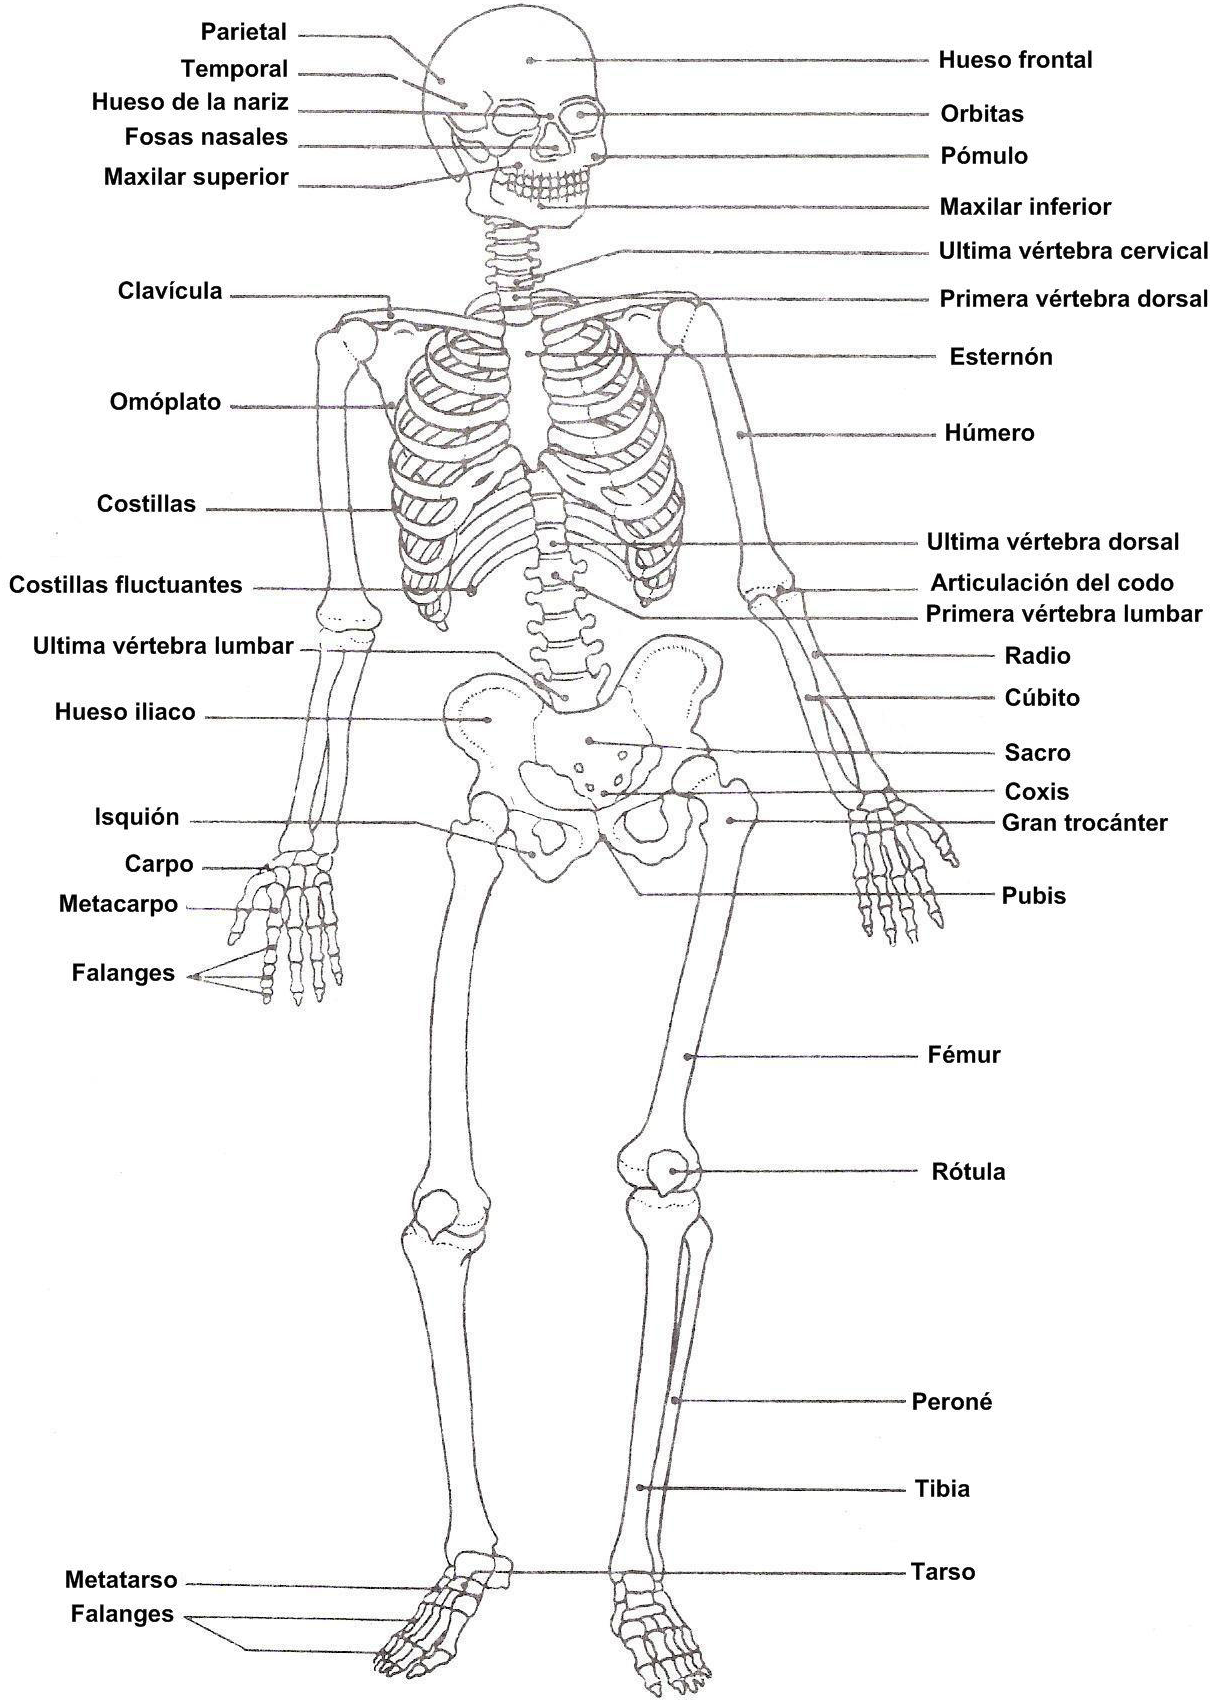
\includegraphics[width=0.35\columnwidth]{images/skeleton.png}
		\caption{Huesos del cuerpo humano}
	\label{fig:skeleton}
\end{figure}

Un hueso est\'a compuesto por un material duro y liviano que contiene componentes org\'anicos e inorg\'anicos formados por c\'elulas vivas dentro de un conjunto org\'anico mineralizado. Los componentes org\'anicos incluyen las c\'elulas (osteoblastos, osteocitos y osteoclastos) y la matriz osteoide. Los componentes org\'anicos, son los responsables de la flexibilidad y tensi\'on que permiten al hueso resistir la torsi\'on y el estiramiento. Sin estos componentes, los huesos seguir\'ian siendo duros pero muy fr\'agiles.

Por otra parte, los componentes inorg\'anicos del hueso representan el 65\% de la masa del mismo, y est\'an formados por microesferas de hidroxiapatita de calcio. Este componente permite obtener una excepcional dureza del hueso. La combinaci\'on de los componentes org\'anicos e inorg\'anicos permiten que los huesos posean caracter\'isticas como durabilidad y dureza sin llegar a ser fr\'agiles.

%%%%%%%%%%%%%%%%%%%%%%%%%%%%%%%%%%%%%%%%%%%%%%%%%%%%%%%%
\subsection{Tipos de hueso}

Un hueso puede ser clasificado por la estructura que posee o por su forma. A continuaci\'on se describen estas dos clasificaciones.

\subsubsection*{Clasificaci\'on por Estructura}

Los huesos tienen una estructura interna en forma de un mallado que var\'ia en cuanto a su densidad en diferentes zonas. La estructura de un hueso puede ser compacta o esponjosa como se muestra en la Figura \ref{fig:esponjosocompacto}. Por ejemplo, la capa externa del hueso cortical es de estructura compacta y comprime una porci\'on importante de masa esquel\'etica. Una estructura esponjosa, se puede observar en el hueso trabecular donde su estructura es similar a un panal de abejas.
\begin{figure}[htb]
	\centering
		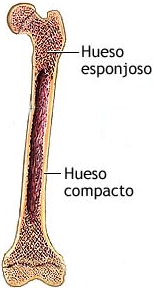
\includegraphics[width=0.20\columnwidth]{images/esponjosocompacto.png}
		\caption{Clasificaci\'on de huesos por su estructura}
	\label{fig:esponjosocompacto}
\end{figure}

\subsubsection*{Clasificaci\'on por Forma}

Los huesos pueden ser clasificados por su forma como largos, cortos, planos o irregulares, como se muestra en la Figura \ref{fig:byshape}. Los huesos largos como el f\'emur, ver Figura \ref{fig:byregion}, son estructuras tubulares que consisten en las siguientes regiones:

\begin{figure}[htb]
  \begin{center}
 \subfigure[]{\label{fig:byshape}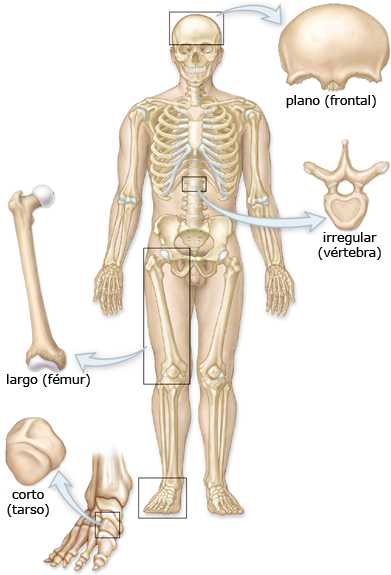
\includegraphics[width=0.40\columnwidth]{images/boneByShape.png}} \hspace{1cm}
    \subfigure[]{\label{fig:byregion}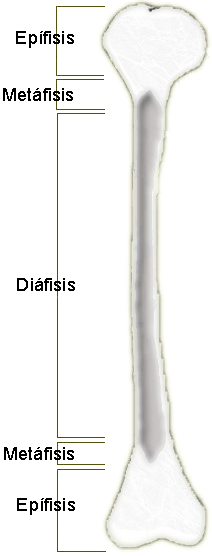
\includegraphics[scale=0.35]{images/femur1.png}}
  \end{center}
  \caption{(a) Clasificaci\'on de huesos por su forma.(b) Regiones de los huesos largos}
  \label{fig:second}
\end{figure}

\subparagraph{Di\'afisis:}El eje central de un hueso largo es llamado di\'afisis. Est\'a localizada entre las met\'afisis y consiste de una pared de hueso compacto y tiene una cavidad hueca medular rellena de m\'edula \'osea. La superficie externa de la di\'afisis est\'a cubierta por el periostio.

\subparagraph{Met\'afisis:}Es una zona intermedia ubicada entre la ep\'ifisis y la di\'afisis. Las placas epifisarias (i.e. placas de crecimiento) se encuentran en las met\'afisis y son responsables del crecimiento y el alargamiento de los huesos durante la infancia.

\subparagraph{Ep\'ifisis:}Est\'a constituida por los 2 extremos del hueso en los que se encuentran las superficies articulares del hueso. Consiste en su mayor\'ia de hueso esponjoso cubierto por una capa relativamente delgada de hueso compacto cortical.

Los huesos cortos, como los huesos de los dedos, la mu\~neca, los huesos del tobillo y la r\'otula, tienen una estructura similar a los huesos largos, excepto que no tienen cavidad medular. Los huesos planos del cr\'aneo y las costillas consisten en dos capas de hueso compacto con una zona de hueso esponjoso situado entre ellos. Por \'ultimo los huesos irregulares son los huesos como las v\'ertebras y la pelvis, que no encajan en ninguna de las categor\'ias anteriores. En el caso particular del f\'emur, \'este es el hueso tubular m\'as largo del cuerpo y est\'a rodeado por la masa muscular m\'as extensa.

%%%%%%%%%%%%%%%%%%%%%%%%%%%%%%%%%%%%%%%%%%%%%%%%%%%%%%
\section{Fractura del hueso}

A pesar de que son muy flexibles y fuertes, los huesos son susceptibles al da\~no. Si se aplica m\'as fuerza en un hueso del que puede soportar, \'este se quiebra. Una ruptura de cualquier tama\~no se conoce como una fractura. La mayor\'ia de las fracturas que se producen antes de la edad adulta son consecuencia de traumatismos excepcionales tales como lesiones deportivas, ca\'idas de altura, accidentes automovil\'isticos y ca\'idas que tuercen o aplastan los huesos.

Las fracturas de hueso se pueden originar por 3 causas principales:

\subparagraph{Traumatismo directo:}El foco de fractura ha sido producido por un golpe directo. La energ\'ia producida se transmite directamente por la piel y las partes blandas. Esta clasificaci\'on tambi\'en abarca las fracturas producidas como consecuencia de una ca\'ida, en las cuales el hueso es el medio de transmisi\'on de la acci\'on de la fuerza y el suelo (u otro elemento contundente), superando la resistencia \'osea.
\subparagraph{Traumatismo indirecto:}El punto de aplicaci\'on de la fuerza est\'a alejado del foco de fractura. En este caso, las fuerzas aplicadas tienden a torcer o angular el hueso. Por ejemplo, la ca\'ida desde una motocicleta, con rotaci\'on de la pierna, produce una fractura a nivel medio de la tibia y el peron\'e, estando las fuerzas aplicada a nivel del pie fijo y de todo el cuerpo en rotaci\'on y ca\'ida.
\subparagraph{Por fatiga:}La fuerza que origina la fractura es aplicada en forma prolongada e intermitente en el tiempo. Por ejemplo, la fractura de marcha que se produce en algunos atletas o reclutas del ej\'ercito, que se produce en el pie.
%\end{enumerate}

\subsection{Tipos}

Pueden ocurrir distintos tipos de fracturas y estas var\'ian de acuerdo a su impacto, van desde una l\'inea muy fina de fractura hasta una fractura compleja formada por dos o m\'as fragmentos de hueso. En una clasificaci\'on b\'asica, las fracturas se pueden clasificar como simples o multifragmentarias. El t\'ermino simple se emplea para describir una sola l\'inea de fractura de un hueso roto con las partes a\'un en su posici\'on anat\'omicamente normal y un da\~no m\'inimo al tejido circundante. Por otra parte, el t\'ermino multifragmentaria se utiliza cuando hay dos o m\'as fragmentos de hueso presente en la fractura. 

Las fracturas tambi\'en pueden describirse como abiertas (tambi\'en conocido como expuestas) y cerradas, como se muestra en la Figura \ref{fig:fracture1}. En una fractura abierta, un hueso roto sobresale al exterior del cuerpo a trav\'es de una herida abierta, dando lugar a lesiones de tejidos blandos de los m\'usculos, tendones, ligamentos, vasos sangu\'ineos y nervios. Con fracturas abiertas, existe un alto riesgo de infecci\'on de los tejidos internos. Una fractura cerrada es una fractura del hueso que se mantiene interna y generalmente se da en combinaci\'on con una lesi\'on de un \'organo, la arteria o nervios.
\begin{figure}[htb]
	\centering
		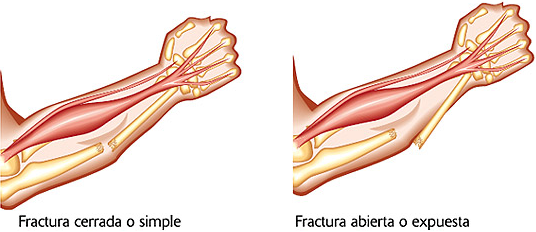
\includegraphics[width=0.60\columnwidth]{images/fractura1.png}
		\caption{Fractura cerrada y fractura abierta}
	\label{fig:fracture1}
\end{figure}

Las fracturas tambi\'en se pueden clasificar en otras categor\'ias: transversal, oblicua, espiral, alas de mariposa o conminuta (ver Figura \ref{fig:fracture2}). Este tipo de clasificaci\'on var\'ia de acuerdo a la forma de la ruptura del hueso y a sus caracter\'isticas: \'angulo, fractura del eje, zona del segmento de hueso, etc. Un tipo adicional de fractura es la fractura por insuficiencia. Las fracturas por insuficiencia son de dos tipos: por estr\'es y osteopor\'otico. Una fractura de estr\'es es una lesi\'on por uso excesivo causado por fuerzas repetitivas o prolongadas contra el hueso, causando una fisura a la forma. Estas fracturas son m\'as frecuentes en las extremidades inferiores como consecuencia de las fuerzas de reacci\'on del suelo en actividades como correr, caminar, marchar, o saltar. Por otro lado, las fracturas osteopor\'oticas son originadas por una enfermedad llamada osteoporosis, la cual disminuye la cantidad de minerales en el hueso, ocasionando la p\'erdida de fuerza en la parte del hueso trabecular y reduciendo la zona cortical por un defecto en la absorci\'on del calcio.

\begin{figure}[htb]
	\centering
		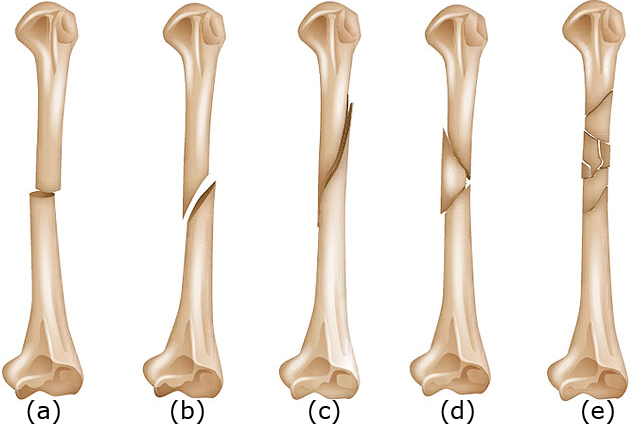
\includegraphics[width=0.50\columnwidth]{images/fracture2.png}
		\caption{Clasificaci\'on de fracturas (a) Transversal (b) Oblicuo (c) Espiral (d) Alas de Mariposa (e) Conminuta}
	\label{fig:fracture2}
\end{figure}

%begin check
\subsection{Incidencia}

En Venezuela, no existe un estudio poblacional del \'area de Salud para la incidencia de fracturas en la poblaci\'on. Una publicaci\'on realizada por el Dr. Strocchia et al. \cite{STRO01} en el a\~no 2001, refleja un estudio con 59 pacientes con el objetivo de evaluar las eventualidades surgidas con diversos m\'etodos de fijaci\'on. Strocchia et al. \cite{STRO01} realizaron el estudio en el Hospital Dr. Victorino Santaella Ru\'iz de Los Teques, en el per\'iodo de Enero 2001 hasta Diciembre 2001. En dicho estudio, se evidenci\'o una alta incidencia en pacientes j\'ovenes con predominio del sexo masculino ($81.35\%$), siendo las heridas por arma de fuego la principal causa ($38.9\%$).

En los Estados Unidos de Norteam\'erica, seg\'un la informaci\'on mostrada en \cite{NAT02}, durante el a\~no 2001 las fracturas representaron el $7,0\%$ del total de lesiones no fatales y enfermedades que motivaron d\'ias de ausencia al trabajo en ese a\~no. Esta categor\'ia incluye tanto fracturas abiertas como cerradas de huesos y dientes. Las fracturas se encuentran entre los problemas ortop\'edicos m\'as frecuentes \cite{DIS05}. Aproximadamente 6,8 millones de ciudadanos estadounidenses se fracturan un hueso al a\~no. En promedio, en los Estados Unidos de Norteam\'erica cada persona vive la experiencia de dos fracturas a lo largo de su vida.

En el caso particular de fractura del f\'emur, en los Estados Unidos de Norteam\'erica durante el a\~no 2001, una de cada 1.157 personas padeci\'o de esta lesi\'on. Dicho valor, equivale al $0.09\%$ de la poblaci\'on total \'o a un total de 235.486 personas.

%end check

%%%%%%%%%%%%%%%%%%%%%%%%%%%%%%%%%%%%%%%%%%%%%%%%
\subsection{Diagn\'ostico}

Al momento de presentarse una fractura, es importante determinar d\'onde se encuentra la misma y cu\'al fue la causa que la origin\'o. Existen m\'ultiples s\'intomas causados por un hueso roto: hematomas, dolor intenso, visibilidad de un hueso o articulaciones fuera de su posici\'on correcta, movilidad limitada, etc.

A pesar de poseer un conjunto de los s\'intomas antes mencionados, las im\'agenes m\'edicas son el mejor m\'etodo disponible actualmente para confirmar la presencia de una fractura. Diversas modalidades de im\'agenes son utilizadas para analizar la estructura \'osea de un paciente, tal como la Tomograf\'ia Computarizada (CT - \textit{Computer Tomography}), Resonancia Magn\'etica (MR - \textit{Magnetic Resonance}) y Ultrasonido (US - \textit{Ultrasound}). Sin embargo, la mayor\'ia de los casos de fractura son diagnosticados utilizando im\'agenes de Rayos-X (\textit{X-Ray}) ya que estas permiten determinar r\'apidamente una anomal\'ia, adem\'as de ser un examen menos costoso para el centro hospitalario. En estos casos, el m\'edico tratante solicita una serie de Rayos-X centrados en el \'area de inter\'es.

La Figura \ref{fig:xray} muestra un esquema con los elementos involucrados en la captura de una imagen de Rayos-X. Las im\'agenes son producidas al colocar una pel\'icula de Rayos-X u otro detector en un lado del hueso fracturado, y una fuente de Rayos-X por el otro (un colimador y tubo de Rayos-X). Durante la exposici\'on, los Rayos-X son absorbidos en gran medida por la mayor\'ia de los materiales densos como los huesos, y en un grado mucho menor por tejidos menos densos como m\'usculos y grasa. Como es explicado en \cite{Hollins01}, la imagen resultante es clara en las \'areas \'oseas donde los Rayos-X fueron absorbidos y oscuras en las zonas de tejido blando donde los Rayos-X no fueron absorbidos.
\begin{figure}[htb]
	\centering
		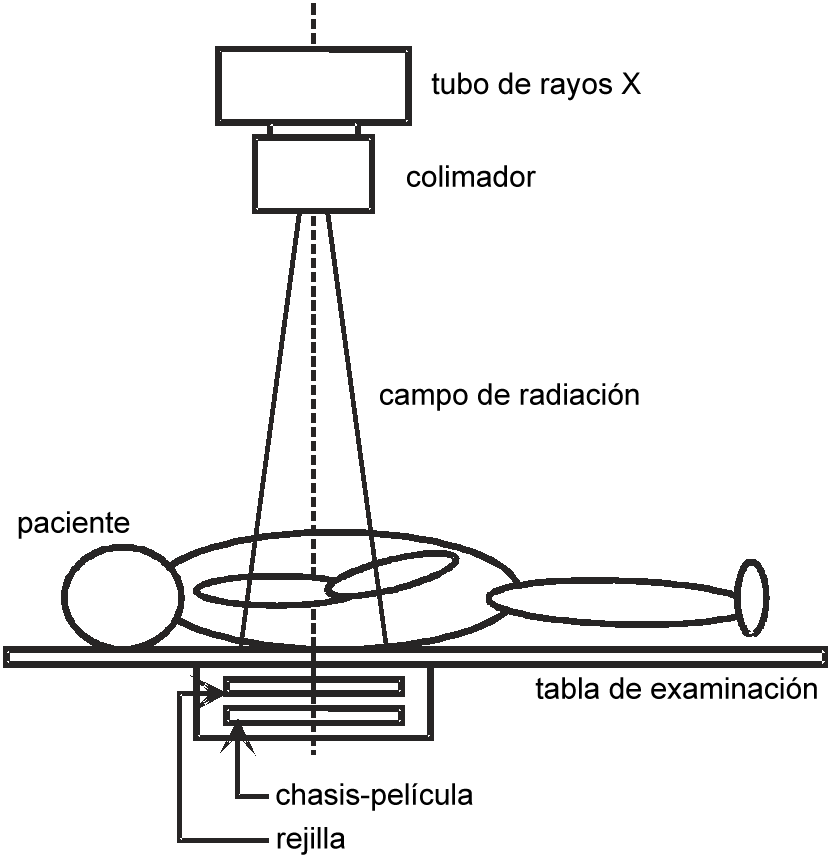
\includegraphics[width=0.40\columnwidth]{images/xray.png}
		\caption{Esquema de un examen de Rayos-X}
	\label{fig:xray}
\end{figure}

La imagen resultante es una proyecci\'on de una estructura tridimensional en un plano bidimensional. Como resultado de ello, pueden existir otras estructuras en el camino de la influencia del haz de Rayos-X y la toma. Esto genera la presencia de superficies solapadas u ocultas tales que complican la detecci\'on de la fractura, por lo que es necesario capturar im\'agenes desde m\'as de un punto de vista. Una vez que se obtiene un n\'umero suficiente de puntos de vista del hueso fracturado, las im\'agenes son analizadas por un radi\'ologo para determinar el lugar y forma de la fractura en el hueso. 

Dos tipos de proyecciones utilizadas muy frecuentemente son la proyecci\'on AP (anteroposterior) y LAT (lateral). La proyecci\'on AP consiste en colocar el paciente mirando hacia el equipo de Rayos-X \'o con una rotaci\'on de 180 grados con respecto a este. Por otro lado, la proyecci\'on LAT consiste en colocar al paciente con un giro de $\pm$ 90 grados con respecto a la parte frontal del equipo. En la Figura \ref{fig:proyeccionAP} se observa una placa de Rayos-X tomada a un t\'orax en una proyecci\'on AP, y en la Figura \ref{fig:proyeccionLAT} se observa el mismo t\'orax en una proyecci\'on LAT.

\begin{figure}[htb]
  \begin{center}
    \subfigure[]{\label{fig:proyeccionAP}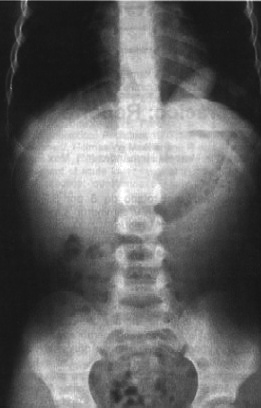
\includegraphics[width=0.20\columnwidth]{images/AP.png}} \hspace{1cm}
    \subfigure[]{\label{fig:proyeccionLAT}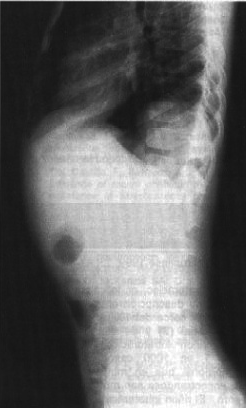
\includegraphics[width=0.20\columnwidth]{images/LAT.png}}
  \end{center}
  \caption{Rayos-X de un t\'orax abdominal simple en proyecci\'on (a) anteroposterior y (b) lateral}
  \label{fig:proyeccion}
\end{figure}

De acuerdo a \cite{SQUIRE69}, las im\'agenes de Rayos-X no son f\'aciles de examinar ya que se requiere de una buena interpretaci\'on de la misma para realizar un diagn\'ostico. Esto incluye tener un conocimiento sobre el lugar donde aparecen las sombras y la intensidad de las mismas de acuerdo a la posici\'on en el momento de la adquisici\'on de la imagen, para as\'i determinar con precisi\'on las caracter\'isticas de la fractura. Adicionalmente, se necesita una habilidad para recrear en 3D (geometr\'ia reconstructiva y espacial) a un paciente mientras se observa una imagen 2D. Finalmente, se analizan las sombras presentes con el objetivo de visualizar su estructura tridimensional y as\'i determinar una clasificaci\'on de la fractura.

%%%%%%%%%%%%%%%%%%%%%%%%%%%%%%%%%%%%%%%%%%%%%%%%
\subsection{Clasificaci\'on}

Una vez confirmada la presencia de una fractura, M\"{u}ller et al. \cite{MULL90} plantean que la lesi\'on en el hueso afectado debe ser reconocida, identificada y descrita utilizando la inspecci\'on de la imagen radiogr\'afica en concordancia con alg\'un esquema ya establecido. Existen diversos esquemas de fracturas, a continuaci\'on se mencionan algunos de ellos:

%%%%%%%%%%%%%%%%%%%%%%%%%%%%%%%%%%%%%%%%%%%%%%%%
\subsubsection{Esquema Salter-Harris}

La clasificaci\'on de Salter-Harris es utilizada principalmente para fracturas tratadas dentro del \'area de pediatr\'ia donde se utiliza una placa de crecimiento (met\'afisis). Este tipo de lesiones es aproximadamente el 15-20\% de las fracturas de f\'emur y tibia y 34\% de las fracturas de mano durante la infancia, seg\'un las estad\'isticas mostradas en \cite{UZE06}. La gran mayor\'ia de estas fracturas se curan sin ninguna alteraci\'on del mecanismo de crecimiento. En este esquema las fracturas son categorizadas en 5 tipos, los cuales se muestran en la Figura \ref{fig:SalterHarris} y se describen en la Tabla \ref{tab:fract}.

\begin{table}[htp]
\center
\begin{tabular}{|c|c|l|}
\hline
Tipo & Frecuencia & Descripci\'on \\ \hline
I & 5\% & Deslizamiento de la fisis \\ 
II & 75\% & Lesi\'on de la met\'afisis y de la fisis \\ 
III & 10\% & Lesi\'on de la ep\'ifisis y de la fisis \\ 
IV & 10\% & Lesi\'on de la met\'afisis, fisis y ep\'ifisis \\ 
V & < 1\% & Lesi\'on por compresi\'on de la fisis (aplastamiento) \\ 
\hline
\end{tabular}
\caption{Descripci\'on  de las categor\'ias del esquema Salter-Harris}
\label{tab:fract}
\end{table}

\begin{figure}[htb]
	\centering
		\includegraphics[width=1.0\columnwidth]{images/SalterHarris2.png}
		\caption{Tipos de fracturas bajo el esquema Salter-Harris}
	\label{fig:SalterHarris}
\end{figure}

%%%%%%%%%%%%%%%%%%%%%%%%%%%%%%%%%%%%%%%%%%%%%%%%
\subsubsection{Esquema Gustilo}

La clasificaci\'on de Gustilo \cite{BROW03} es para fracturas abiertas y est\'a basada en el grado de lesi\'on de las partes blandas. Esta clasificaci\'on plantea 3 grandes grupos que indican la cantidad de tejido blando da\~nado que es asociado con la fractura. La Tabla \ref{tab:gustilo} muestra la descripci\'on de cada uno de estos grupos.

\begin{table}[htp]
\center
\begin{tabular}{|c| p{13cm}|}
\hline
Grupo & Descripci\'on \\ \hline
1 & La herida es peque\~na, generalmente puntiforme, con escasa contusi\'on o deterioro de las partes blandas (piel, celular, m\'usculos, etc.). El traumatismo es de baja energ\'ia. \\
\hline
2 & La herida es amplia y la exposici\'on de las partes blandas profundas es evidente, pero el da\~no f\'isico de ellas es moderado. El traumatismo es de mediana energ\'ia. \\
\hline
3 & La herida es de gran tama\~no en extensi\'on y profundidad: a nivel cut\'aneo, celular y muscular. Generalmente hay da\~no importante de estructuras neuro-vasculares. El traumatismo es de alta energ\'ia. \\ 
\hline
\end{tabular}
\caption{Descripci\'on  de los grupos del esquema Gustilo}
\label{tab:gustilo}
\end{table}

%%%%%%%%%%%%%%%%%%%%%%%%%%%%%%%%%%%%%%%%%%%%%%%%
\subsubsection{Esquema Tscherne}

La clasificaci\'on de Tscherne \cite{STAN07} fue dise\~nada en 1982 y es s\'olo para fracturas cerradas. Se basa en un concepto subjetivo sobre la condici\'on general de la lesi\'on hecha con observaci\'on del m\'edico, conocimiento del mecanismo de la lesi\'on y la severidad de la fractura. Se basa en 4 grados de severidad: Grado 0, 1, 2 y 3. El nivel de severidad Grado 0 implica un da\~no m\'inimo sobre el tejido blando, causado por violencia indirecta y un patr\'on simple. Por otra parte, el nivel de severidad Grado 3 define una contusi\'on severa sobre el tejido, destrucci\'on del m\'usculo, lesiones vasculares, etc., causado por un impacto de alta energ\'ia.

%%%%%%%%%%%%%%%%%%%%%%%%%%%%%%%%%%%%%%%%%%%%%%%%
\subsubsection{Esquema AO}

Actualmente, la clasificaci\'on AO (siglas en alem\'an para \textit{Arbeitsgemeinschaft f\"{u}r Osteosynthesefragen}) para fracturas, es la clasificaci\'on m\'as aceptada internacionalmente. Se basa en clasificar la fractura de acuerdo a su ubicaci\'on y caracter\'istica morfol\'ogica. Seg\'un este esquema, se requiere de 4 letras/n\'umeros para ubicar con gran precisi\'on una fractura y su severidad (sin tomar en cuenta los subgrupos y la escala de severidad). 

La ubicaci\'on es asignada por dos n\'umeros, como se muestra en la Figura \ref{fig:AO}, que indica en cu\'al hueso y en cu\'al segmento ocurri\'o la fractura. La Tabla \ref{tab:AO} muestra la clasificaci\'on para los huesos.
\begin{table}
\begin{center}
\begin{tabular}{|c|l|}
\hline
Clasificaci\'on & Hueso \\ \hline
1 & H\'umero\\ 
2 & Radio/C\'ubito\\ 
3 & F\'emur/R\'otula\\ 
4 & Tibia/Peron\'e\\ 
5 & Columna vertebral\\ 
6 & Pelvis/Acetabular\\ 
7 & Huesos de la mano\\
8 & Huesos del pie\\ 
9 & Huesos craneomaxilofaciales\\ 
\hline
\end{tabular}	
%\caption{none}
\end{center}
\caption{Numeraci\'on de los huesos seg\'un el esquema de clasificaci\'on AO}
\label{tab:AO}
\end{table}


\begin{figure}[htb]
	\centering
		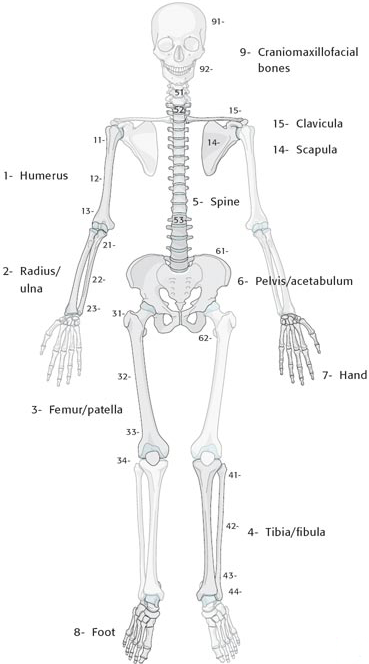
\includegraphics[width=0.35\textwidth]{images/ao_classification.png}
		\caption{Clasificaci\'on AO para la numeraci\'on de acuerdo a la ubicaci\'on anat\'omica de la fractura. Informaci\'on tomada de \cite{REF_AO}}
	\label{fig:AO}
\end{figure}

Esta notaci\'on alfanum\'erica sirve como gu\'ia al cirujano para la valoraci\'on de la fractura con una alta precisi\'on. Los huesos largos, se dividen en tres segmentos: 1=proximal, 2=di\'afisis y 3=distal. Una vez seleccionados ambos n\'umeros, entra en una clasificaci\'on por tipo de fractura (A=simple, B=en cu\~na y C=compleja). Luego, la fractura es dividida en tres grupos que miden la escala de severidad de la misma (1,2,3). En la Figura \ref{fig:AOfemur} se muestra la clasificaci\'on AO para el f\'emur en segmento diafisial.
\begin{figure}[htb]
	\centering
		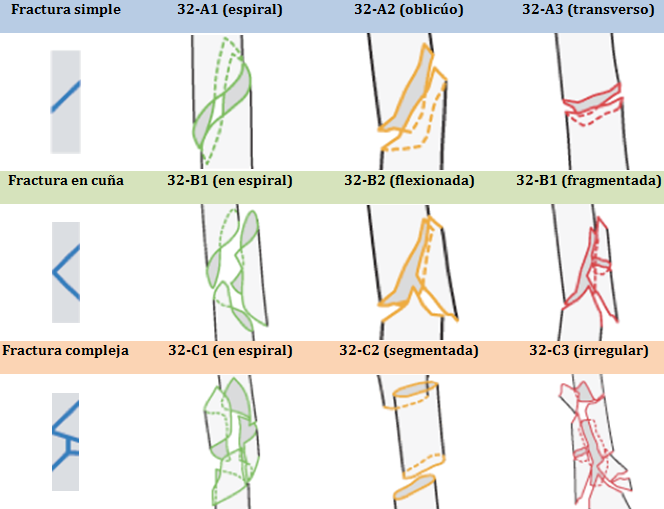
\includegraphics[width=0.7\textwidth]{images/ao_femur.png}
		\caption{Clasificaci\'on AO que corresponde a una fractura tipo 32}
	\label{fig:AOfemur}
\end{figure}

El esquema de clasificaci\'on de AO es recomendado por M\"{u}ller et. al. \cite{MULL90} al definirlo como una clasificaci\'on cl\'inicamente relevante, simple, reproducible y proporciona una buena estimaci\'on de los resultados cl\'inicos.

%%%%%%%%%%%%%%%%%%%%%%%%%%%%%%%%%%%%%%%%%%%%%%%%
\subsubsection{Otros esquemas}

Se pueden encontrar otros esquemas de clasificaci\'on que dependen exclusivamente del lugar de la lesi\'on. Seg\'un Koval y Zuckerman \cite{KOV02}, las fracturas de la pelvis pueden ser clasificadas bajo el esquema de Young y Burgess, las fracturas de la clav\'icula con la clasificaci\'on de Allman y las fracturas de la meseta tibial con la clasificaci\'on de Schatzker. Estas clasificaciones s\'olo son relevantes para su particular regi\'on anat\'omica, por lo que no pueden ser comparadas con las dem\'as que pueden ser aplicadas a todo el cuerpo humano.

%%%%%%%%%%%%%%%%%%%%%%%%%%%%%%%%%%%%%%%%%%%%%%%%
\subsection{Tratamiento}

Una fractura de hueso sana naturalmente a trav\'es de un proceso fisiol\'ogico siempre que se encuentre lo suficientemente inmovilizado. La insuficiente inmovilizaci\'on puede resultar en una cicatrizaci\'on inadecuada del hueso, y la formaci\'on de una pseudoartrosis. En consecuencia,  existen tres opciones principales para tratamiento en la reparaci\'on de fracturas de huesos, planteadas en \cite{MORO99}, donde todas requieren la inmovilizaci\'on de las piezas \'oseas fracturadas. 

Para tratar una fractura se efect\'ua un proceso de \textit{reducci\'on} que consiste en colocar los fragmentos de hueso en su alineaci\'on correcta. En las fracturas simples, el m\'etodo m\'as com\'un es la reducci\'on cerrada bajo anestesia, seguida por la aplicaci\'on de un yeso alrededor del exterior de la extremidad.

En fracturas m\'as severas, se emplea la reducci\'on abierta de la fracturas y la fijaci\'on interna (ver Figura \ref{fig:AOfijador}(a)). Esta t\'ecnica consiste en una cirug\'ia para colocar barras de metal, tornillos o placas por debajo de la piel y as\'i permitir que el hueso sane.
\begin{figure}[htb]
	\centering
		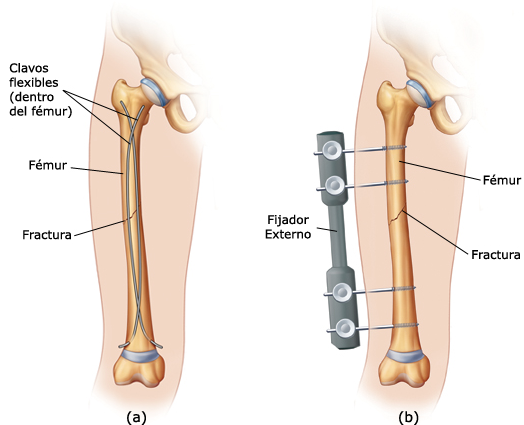
\includegraphics[width=0.55\textwidth]{images/fijadores.png}
		\caption{Inmovilizaci\'on de una fractura por (a) fijaci\'on interna y (b) fijaci\'on externa}
	\label{fig:AOfijador}
\end{figure}

Este procedimiento se recomienda para las fracturas complicadas que no se pueden reducir por bastidor, o en los casos en que el uso a largo plazo de una f\'erula no es recomendable. Por ejemplo, para las fracturas diafisiarias femorales donde se utiliza una placa, \'esta debe ser anat\'omica y su fijaci\'on debe quedar garantizada y es por ello que se emplean tornillos. Al mismo tiempo, un tratamiento de enclavado endomedular tambi\'en puede ser aplicado para este tipo de fracturas ya que tratan con \'exito la mayor parte de estas fracturas ya sean de trazo transversal, oblicuo, espiroideo, segmentario o conminuto.

Por \'ultimo, la reducci\'on de fracturas abiertas y fijaci\'on externa (ver Figura \ref{fig:AOfijador}(b)) consiste en una cirug\'ia para reparar la fractura y la colocaci\'on de un dispositivo de fijaci\'on externa en la extremidad con la fractura. Este dispositivo es un marco externo que sostiene los huesos y los mantiene en su posici\'on correcta mientras se curan. Esta t\'ecnica se aplica generalmente a las fracturas complejas que no pueden ser reparadas mediante reducci\'on abierta y fijaci\'on interna.

%%% End: 
		\chapter{Sistemas CAOS para planificaci\'on preoperatoria}

%%%%%%%%%%%%%%%%%%%%%%%%%%%%%%%%%%%%%%%%%%%%%%%%%%%
\section{Planificaci\'on preoperatoria}

La planificaci\'on preoperatoria o planificaci\'on prequir\'urgica es una disciplina sumamente importante que debe ser realizada por todos los cirujanos ortop\'edicos como requisito indispensable para llevar a cabo un determinado procedimiento quir\'urgico con excelentes resultados.

\begin{quote}
\textit{
	El tiempo que el cirujano ortopedista dedique a efectuar una cuidadosa planificaci\'on preoperatoria tiene una importancia decisiva y a menudo determina el \'exito o fracaso de una operaci\'on
	}
\end{quote}
\begin{center} \footnotesize \textit{Joseph Schatzker. Tratamiento Quir\'{u}rgico de las fracturas \cite{SCHA98}}. \end{center}

Como se describe en \cite{RUEDI03}, la planificaci\'on preoperatoria ortop\'edica es un procedimiento indispensable que debe realizarse previo a la intervenci\'on quir\'urgica y cuyos objetivos son: determinar el resultado final de la cirug\'ia y establecer la t\'actica quir\'urgica a seguir en el procedimiento quir\'urgico. 

La planificaci\'on preoperatoria para una cirug\'ia plantea la realizaci\'on de calcos preoperatorios, como se muestra en la Figura \ref{fig:planificacion}. Los calcos permiten entender la complejidad de la fractura, la forma de reducci\'on de la misma, las acciones a seguir para la reducci\'on y la elecci\'on del implante necesario.
\begin{figure}[htbp]
  \begin{center} \subfigure[]{\label{fig:plan1}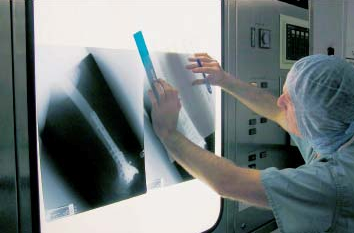
\includegraphics[width=0.45\columnwidth]{images/plan1.png}}  \subfigure[]{\label{fig:plan2}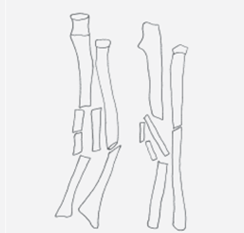
\includegraphics[width=0.31\columnwidth]{images/plan2.png}}   
  \end{center}
  \caption{Procedimiento manual para la creaci\'on de un calco preoperatorio. (a) Creaci\'on del calco sobre un negatoscopio (b) Calco obtenido}
  \label{fig:planificacion}
\end{figure}

En ciertos procedimientos quir\'urgicos, la planificaci\'on preoperatoria es parte integral de una cirug\'ia. Un ejemplo de ello, se muestra en \cite{EGGLI98,BENE03} donde se aplica planificaci\'on preoperatoria para la colocaci\'on de una pr\'otesis de cadera. Antes de la operaci\'on, es importante conocer ciertos factores previos: tipo y tama\~no de la pr\'otesis, posici\'on y orientaci\'on correcta de los implantes, tama\~no del acet\'abulo y del hueso. Al mismo tiempo, esta informaci\'on permite indicar los procedimientos a realizar durante la cirug\'ia y prever cualquier inconveniente. Estos procedimientos traen como resultado la reducci\'on del tiempo de cirug\'ia y garantizar, con un alto nivel de probabilidad, resultados satisfactorios.

Para tener \'exito en el resultado final de la cirug\'ia, R\"{u}edi et al. \cite{RUEDI03} sugieren que se deben realizar las siguientes acciones:
\begin{itemize}
	\item Tomar en cuenta los factores iniciales del contacto m\'edico-paciente.
	\item Crear una historia m\'edica completa.
	\item Realizar una evaluaci\'on preoperatoria.	
	\item Obtener radiograf\'ias para la planificaci\'on (preferiblemente sin inmovilizadores que obstaculicen la visi\'on adecuada).
	\item Si es necesario, realizar estudios especiales como CT, MRI, estudios de laboratorio, entre otros.
	\item Crear una planificaci\'on previa a la operaci\'on.
\end{itemize}

%%%%%%%%%%%%%%%%%%%%%%%%%%%%%%%%%%%%%%%%%%%%%%%%%%%
\subsection{Procedimiento para su realizaci\'on}

La planificaci\'on consiste en realizar un calco de los segmentos de fractura y del hueso, para as\'i tener una gu\'ia correspondiente a la anatom\'ia de la zona a tratar del paciente. De esta forma, el calco representa la herramienta de trabajo construida por el m\'edico traumat\'ologo para el proceso de fijaci\'on de la fractura (i.e. reconstrucci\'on del hueso). En una fractura, el equipo necesario para realizar las planificaciones se puede resumir en:
\begin{enumerate}
	\item Radiograf\'ias adecuadas: Estas radiograf�as opcionalmente incluyen el lado sano. El lado sano sirve para realizar comparaciones con respecto al lado fracturado, tomando en cuenta los factores de simetr\'ia del cuerpo humano.
	\item Papel para calcos: Es un papel especial (semitransparente) sobre el cual se dibujar\'a la imagen de los trazos de una fractura.
	\item Plantillas de los implantes: Conjunto de las posibles plantillas (\textit{templates}) de implantes (tornillos, clavos, placas, etc.) que puede necesitar una fractura. Cada fabricante de material quir\'urgico, e.g. tornillos, mantiene una librer\'ia de sus productos y \'estos son entregados a los Centros Hospitalarios. En la Figura \ref{fig:plantilla}, se puede observar una plantilla de tornillos.
	\item Goni\'ometro: Instrumento utilizado para medir valores angulares y rangos articulares. Existen m\'ultiples tipos de goni\'ometros, entre los que se destacan los goni\'ometros de dos brazos de eje com\'un y un cuadrante dividido en grados, que son los m\'as utilizados (ver Figura \ref{fig:goniometro}). Tambi\'en existen los goni\'ometros que se basan en la indicaci\'on permanente de la vertical; goni\'ometros que utilizan la desviaci\'on magn\'etica y goni\'ometros electr\'onicos. 
	\item L\'apices o marcadores de colores: Para poder realizar el trazo del calco.
	\item Negatoscopio con luz adecuada: Aparato constituido por una placa transl\'ucida colocada delante de una fuente luminosa, utilizada para examinar las radiograf\'ias. Es sobre este aparato donde son realizados los calcos.
\end{enumerate}

\begin{figure}[htbp]
	\centering
	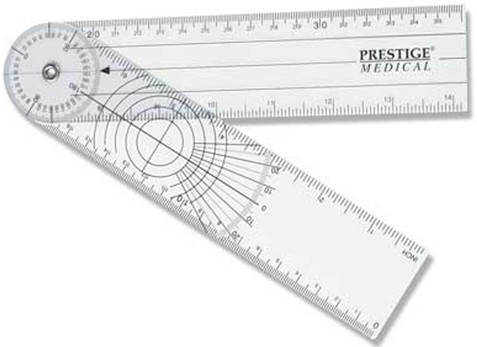
\includegraphics[width=.3\columnwidth]{images/goniometro.png}
	\caption{Goni\'ometro de dos brazos}
	\label{fig:goniometro}
\end{figure}

La elecci\'on del procedimiento quir\'urgico es determinada por las caracter\'isticas de la fractura u osteotom\'ia; hueso, regi\'on, tipo de trazo, desviaciones  angulares, rotaciones, acortamientos, n\'umero de fragmentos, tama\~no de los fragmentos  y las condiciones de los tejidos blandos.
 
La selecci\'on del implante o dispositivo adecuado para la osteos\'intesis debe incluir las acciones a seguir en la cirug\'ia, el abordaje quir\'urgico, el tipo de dispositivo, sus dimensiones, tipo de bloqueo (si lo requiere), dimensiones de los tornillos, orden de colocaci\'on, etc. Para las fracturas diafisiarias en las que est\'a indicada la fijaci\'on con un clavo intramedular bloqueado, se necesita una planificaci\'on gr\'afica preoperatoria poco detallada. Las variables que hay que determinar de acuerdo a lo expuesto en \cite{RUEDI03} son: la longitud y el di\'ametro del clavo intramedular, el fresado o no del canal endomedular y el tipo de bloqueo. La osteos\'intesis con placa requiere una planificaci\'on m\'as detallada, los puntos que deben considerarse son: la correcta longitud, alineaci\'on y rotaci\'on del hueso, el tipo y longitud de la placa, el n\'umero de tornillos y su funci\'on espec\'ifica (compresi\'on interfragmentaria o a trav\'es de la placa). Por \'ultimo, es importante destacar que la planificaci\'on preoperatoria de fracturas que comprometen las superficies articulares es m\'as exigente que las fracturas diafisiarias, puesto que requieren una reducci\'on anat\'omica exacta.

%%%%%%%%%%%%%%%%%%%%%%%%%%%%%%%%%%%%%%%%%%%%%%%%%%%
\subsection{Estrategia quir\'urgica}

En la estrategia quir\'urgica el cirujano ortopedista debe enumerar los pasos a seguir para el procedimiento con el fin de evitar distracciones y para el conocimiento del equipo quir\'urgico. De esta forma dicho equipo estar\'a mejor preparado para resolver los problemas que se puedan presentar. La estrategia quir\'urgica debe estar en el calco de la planificaci\'on preoperatoria, como se observa en la Figura \ref{fig:planificacion_completa}, y debe contener los siguientes puntos:

\begin{figure}[htb]
	\centering
	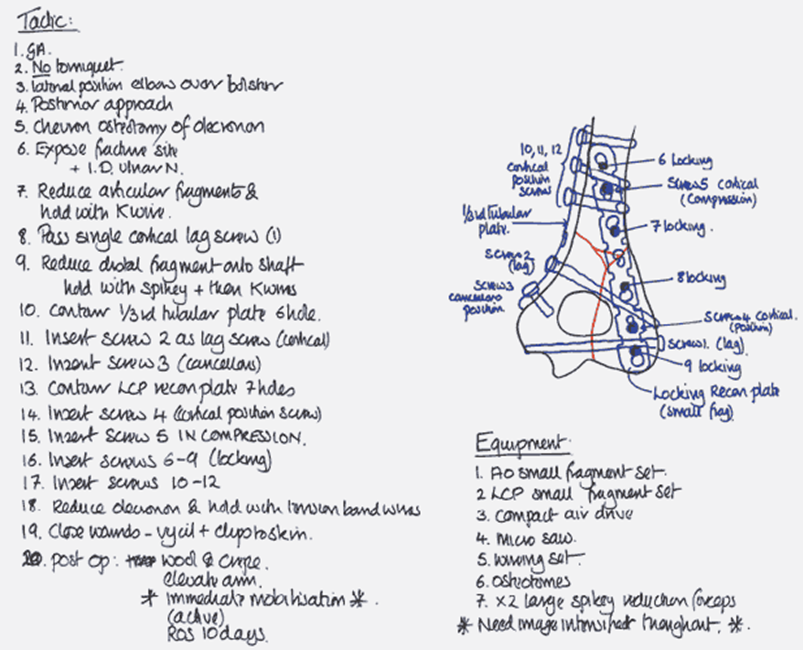
\includegraphics[width=.65\columnwidth]{images/planificacioncompleta.png}
	\caption{Calco de una fractura con la informaci\'on completa antes de la cirug\'ia}
	\label{fig:planificacion_completa}
\end{figure}

\begin{itemize}
	\item Paciente: Nombre y apellido, edad, uso de torniquete, posici\'on del paciente, uso de mesa radiol\'ucida.
	\item Procedimiento: Incluye los procedimientos a realizar durante la cirug\'ia, es decir, las acciones que el m\'edico va a realizar en la operaci\'on (e.g. selecci\'on del tipo de bistur\'i y n\'umero de incisiones, entre otros). Adem\'as incluye el tipo de reducci\'on a aplicar, implantes a emplear y la selecci\'on del equipo a utilizar para la colocaci\'on de implantes.
	\item Equipos Adicionales: Radiograf\'ias transoperatorias (radiograf\'ias tomadas durante la cirug\'ia) empleando un intensificador de im\'agenes, artroscopio, etc.
	\item Cuidados Postoperatorios: Uso de yesos, f\'erulas, pr\'otesis o vendajes en el postoperatorio inmediato.
\end{itemize}

Existen diversas t\'ecnicas de planificaci\'on preoperatoria, entre las que se destacan:
	\subparagraph{Superposici\'on Directa:} Utilizada en las planificaciones de fracturas diafisiarias. Se realiza el calco de los fragmentos fracturados en una proyecci\'on antero-posterior (AP), cada uno en hojas separadas. En otra hoja se traza una l\'inea recta (eje del hueso) y se colocan los fragmentos que son ensamblados para obtener el resultado final.
	\subparagraph{Superposici\'on utilizando la imagen del lado sano:} Se requiere la radiograf\'ia del lado sano y se procede a realizar el calco del lado fracturado tomando en cuenta los fragmentos y rotaciones, dibuj\'andolas en otro color. Luego se realiza la colocaci\'on de los fragmentos dibujados en la radiograf\'ia del lado sano para hacerlos coincidir. Otra forma es realizar la colocaci\'on de los fragmentos y posteriormente superponerla a la radiograf\'ia del lado sano para evaluar la colocaci\'on adecuada de los fragmentos, una vez que se tenga la reducci\'on de los mismos, se utilizan las plantillas de implantes y se completa el calco seg\'un la elecci\'on del cirujano ortopedista.
	\subparagraph{Superposici\'on utilizando los ejes fisiol\'ogicos:} Es una metodolog\'ia aplicable a aquellas fracturas periarticulares (fracturas producidas cercanas a una articulaci\'on), como es el caso de las fracturas supracond\'ileas de f\'emur las cuales son fracturas periarticulares de la porci\'on distal del f\'emur.
En una fractura distal de f\'emur se usa la plantilla para marcar los ejes anat\'omicos  y mec\'anicos del f\'emur y la tibia. Posterior a esto, se dibujan los fragmentos de la fractura y se superponen a la plantilla inicial, para hacer coincidir los ejes del f\'emur y la tibia y as\'i lograr la alineaci\'on de la rodilla. Una vez colocados todos los fragmentos reducidos se procede a la colocaci\'on del implante. \\

Particularmente, en este documento trataremos el caso de la planificaci\'on preoperatoria empleando la t\'ecnica de superposici\'on directa.

%%%%%%%%%%%%%%%%%%%%%%%%%%%%%%%%%%%%%%%%%%%%%%%%%%%
\section{Sistemas CAD}

Actualmente solo algunos cirujanos ortop\'edicos llevan a cabo dichas planificaciones, puesto que se requiere de material adicional y una inversi\'on considerable de tiempo para su realizaci\'on. Los sistemas de Diagn\'ostico Asistido por Computador (\textit{CAD - Computer Aided Diagnosis}) son excelentes herramientas para que los m\'edicos realicen diagn\'osticos m\'as acertados en un tiempo m\'as corto. Cada vez es m\'as frecuente la presencia de estos sistemas en el campo de la medicina, y particularmente existe un gran crecimiento en el \'area de Radiolog\'ia \cite{GIGE00}.

El concepto del CAD es amplio y general como herramienta de asistencia a los radi\'ologos, proporcionando una ``segunda opini\'on'' provista por el computador. Este aspecto, expuesto por Doi en \cite{DOI07}, es la principal diferencia con los sistemas de Diagn\'ostico Automatizado por Computador (\textit{Automated Computer Diagnosis}), los cuales son utilizados para diagnosticar autom\'aticamente cualquier condici\'on de salud-enfermedad (lesi\'on, s\'indrome, entidad nosol\'ogica, etc.). En un sistema CAD siempre el radi\'ologo tomar\'a la decisi\'on final.
 
Las investigaciones en el \'area del Diagn\'ostico Asistido por Computador \cite{HUANG07} se iniciaron en 1980 y han ido evolucionando gradualmente como una herramienta de apoyo cl\'inico. En el \'area de mamograf\'ia, los sistemas CAD se han convertido en una herramienta de rutina para la detecci\'on de c\'anceres de mama en muchos centros m\'edicos. Un gran n\'umero de sistemas CAD en Estados Unidos y Europa \cite{DOI07}, son utilizados para la detecci\'on temprana del c\'ancer de mama en las mamograf\'ias. Algunos sistemas CAD son utilizados para el registro de im\'agenes \cite{ZITO03} (\textit{image registration}), interacciones virtuales, visualizaci\'on, simulaci\'on y entrenamiento.

Por ejemplo, para los casos de entrenamiento y pr\'acticas educativas para estudiantes de medicina, Blyth et al. \cite{BLYT06} ofrecen una herramienta que simula escenarios virtuales a los futuros cirujanos. La necesidad de una simulaci\'on viene determinada por la complejidad de ciertas regiones del cuerpo humano, como la craniofacial o la regi\'on card\'iaca. Es muy importante que estructuras vitales del cuerpo humano no sean da\~nadas durante una operaci\'on, lo cual puede lograrse con el uso de sistemas de este tipo.

En el 2002, Bourquain et al. \cite{BOUR02} desarrollaron (\textit{HepaVision2}), una aplicaci\'on para la planificaci\'on preoperatoria de transplantes y cirug\'ias de h\'igado. \textit{HepaVision2} es una herramienta que trabaja con im\'agenes en formato DICOM \cite{REF_DICOM} (\textit{Digital Imaging and Communication in Medicine}) siendo capaz de realizar una segmentaci\'on del h\'igado empleando el algoritmo \textit{livewire} \cite{MORT95} de detecci\'on semiautom\'atica de bordes. Adem\'as, realiza el c\'alculo del volumen del h\'igado y las venas hep\'aticas que permiten determinar los tumores. Esta versi\'on del software trabaja sobre PCs basadas en \textit{Windows} y provee un m\'odulo de an\'alisis de riesgo de operaci\'on en el paciente a tratar.

%%%%%%%%%%%%%%%%%%%%%%%%%%%%%%%%%%%%%%%
\subsection{Cirug\'ia Ortop\'edica Asistida por Computador}

Diversos software de apoyo al cirujano para la reducci\'on de fracturas en extremidades inferiores son utilizados desde hace varios a\~nos, un ejemplo de ello se muestra en  \cite{TOCKUS98, NAKA24}. Los sistemas CAD de planificaci\'on preoperatoria de cirug\'ias del sistema muscoesquel\'etico, son conocidos como CAOS (\textit{Computer Aided Orthopaedic Surgery}) los cuales son foco de investigaci\'on en diversas partes del mundo \cite{BRAN99, LANG98, RADE98, MART00}.

Al realizar la planificaci\'on preoperatoria con \'estas herramientas, el proceso se torna m\'as preciso y repetible que los m\'etodos convencionales/tradicionales, como el uso de plantillas mostrado en la Figura \ref{fig:plantilla}. 
\begin{figure}[htb]
	\centering
	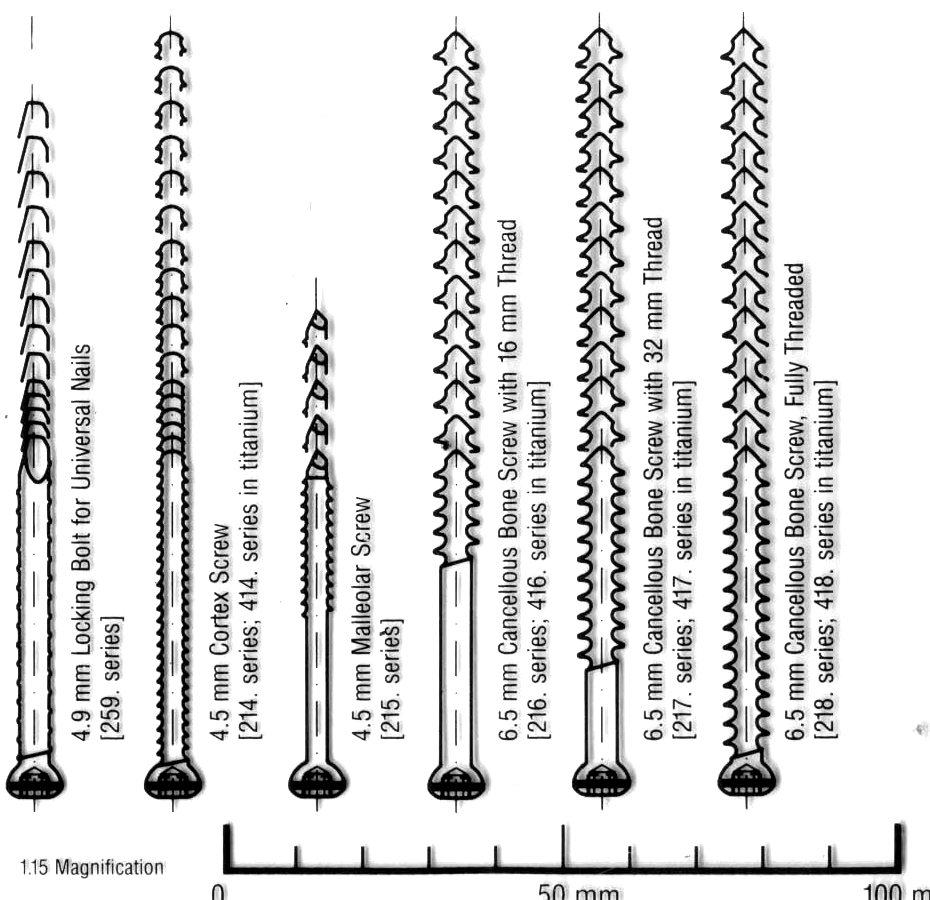
\includegraphics[width=.4\columnwidth]{images/plantillas.png}
	\caption{Un ejemplo de una plantilla (\textit{template}) de tornillos utilizados en una planificaci\'on}
	\label{fig:plantilla}
\end{figure}

Las plantillas (\textit{templates}) son implantes bases construidos por un fabricante bajo diversos materiales y con diferentes medidas. Los implantes que se muestran en las plantillas, sirven de gu\'ia exacta al momento de realizar una reducci\'on y fijaci\'on interna para un paciente. El almacenamiento de estas plantillas se realiza de forma manual bajo criterio propio del Departamento de Radiolog\'ia. Al momento de utilizar una plantilla, es importante conocer la categor\'ia de la fractura as\'i como un diagn\'ostico previo con el fin de determinar su utilizaci\'on \'o no.

Es importante destacar que para la realizaci\'on manual de una reducci\'on de fractura se requiere una inversi\'on de tiempo. Si la inversi\'on de tiempo fuese menor para cada caso de fractura que requiera cirug\'ia, entonces los costos del centro hospitalario se reducen de forma considerable ya que se obtiene mayor tiempo productivo de los m\'edicos cirujanos.

%%%%%%%%%%%%%%%%%%%%%%%%%%%%%%%%%%%%%%%
\subsection{Antecedentes de sistemas CAOS}

Al momento de una cirug\'ia, la elecci\'on del procedimiento quir\'urgico viene determinado por las caracter\'isticas de la fractura u osteotom\'ia: hueso, regi\'on, tipo de trazo, desviaciones angulares, rotaciones, acortamientos, n\'umero de fragmentos, tama\~no de los fragmentos y las condiciones de los tejidos blandos. Dada la cantidad de factores a considerar para dicho procedimiento, R\"{u}edi et al. \cite{website:ruedi} sugieren la creaci\'on de un plan para la cirug\'ia que incluya todos los pasos a realizar de forma ordenada durante el acto quir\'urgico. 

La literatura relacionada con sistemas CAD para fracturas es poca, pero existen trabajos relevantes centrados en la detecci\'on de osteoporosis  y estimaci\'on de la edad de huesos. Uno de los trabajos de mayor aporte en el \'area de detecci\'on de fracturas en huesos largos fue el realizado por Tian et al. \cite{TIAN03} en el 2003, los cuales desarrollaron un algoritmo para detectar las fracturas en el f\'emur y el radio. 

El m\'etodo descrito por Tian et al. \cite{TIAN03} detecta una fractura en el f\'emur solamente en el cuello del mismo. Su t\'ecnica calcula el \'angulo entre el eje del cuello del f\'emur y el eje del f\'emur, llamado \'angulo NSA (\'Angulo del Cervico Diafisiario - \textit{Neck-Shaft Angle}), y trabaja sobre im\'agenes de CT en formato DICOM. Esta medida del \'angulo es realizada en tres etapas: la primera etapa consiste en la extracci\'on del contorno del f\'emur, ver Figura \ref{fig:tian}, la segunda etapa se refiere al c\'alculo del \'angulo NSA, y la tercera es la clasificaci\'on del \'angulo obtenido. La extracci\'on del contorno del f\'emur descrita por Tian et al. \cite{TIAN03}, utiliza la detecci\'on de bordes propuesta por Canny \cite{CANNY86}, la transformada de Hough \cite{DUDA72} y un modelo de Contornos Activos \cite{KASS88}.
\begin{figure}[htb]
	\centering
	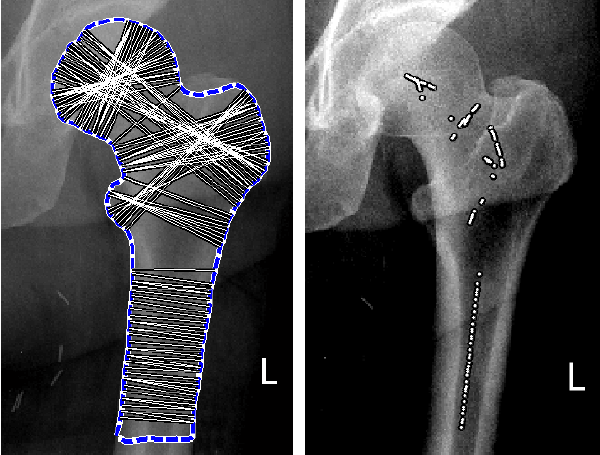
\includegraphics[width=.5\columnwidth]{images/tian.png}
	\caption{L\'ineas encontradas en la detecci\'on del contorno del fem\'ur y l\'ineas gu\'ias para determinar la l\'inea central del fem\'ur. Imagen extra\'ida de \cite{TIAN03}}
	\label{fig:tian}
\end{figure}

En el a\~no 2004 Yap et al. \cite{YAP04} mejoran el m\'etodo aplicado por Tian et al. \cite {TIAN03} para la detecci\'on de fracturas en el f\'emur. Ellos trabajan igualmente sobre im\'agenes de CT, incluyendo el an\'alisis de la perturbaci\'on de los patrones presentes en la trabecular del cuello femoral. De la misma forma, su m\'etodo consiste en 3 etapas: 
\begin{enumerate}
	\item La extracci\'on del contorno del f\'emur.
	\item El an\'alisis de la textura trabecular.
	\item Clasificaci\'on de la fractura.
\end{enumerate}

Para la extracci\'on del f\'emur en la imagen utilizaron un Modelo de Contornos Activo (\textit{snake}) con flujo del vector gradiente. Los resultados obtenidos en este trabajo arrojaron un 84.6\% de exactitud en la detecci\'on de fracturas.

Los m\'etodos mencionados anteriormente producen resultados aceptables, pero tienen como desventaja que solamente trabajan en fracturas localizadas en el cuello femoral y no pueden ser adaptados para otros huesos. Otro factor desfavorable con respecto a estos m\'etodos es originado por el uso de Contornos Activos, porque est\'a t\'ecnica requiere que el m\'edico coloque los puntos iniciales del Contorno Activo y ajuste el modelo la cantidad de veces que sea necesario hasta lograr los resultados esperados.

Una mejora a estos m\'etodos fue introducida por Lim et al. \cite{LIM04} en el 2004, donde se modifica el algoritmo de extracci\'on del contorno propuesto por Tian et al. \cite{TIAN03} incluyendo Campos Aleatorios de Markov (\textit{MRF - Markov Random Fields}) e intensidad en la direcci\'on del gradiente (\textit{IGD - Intensity Gradient Direction}) al m\'etodo existente del NSA y tambi\'en incluyendo mapas de orientaci\'on Gabor (\textit{GO - Gabor Orientation}) \cite{AKDE05}. Adem\'as, Lim et al. \cite{LIM04} modificaron la clasificaci\'on planteada en \cite{YAP04}, y consiguieron una detecci\'on de fracturas del 92.2\% de exactitud y 1\% de detecci\'on de fracturas cuando en realidad no exist\'ian (falso positivo). Un ejemplo de la detecci\'on de fracturas se puede observar en la Figura \ref{fig:lim}.
\begin{figure}[htb]
	\centering
	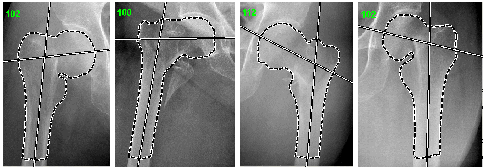
\includegraphics[width=.75\columnwidth]{images/fracturedfemur.png}
	\caption{Identificaci\'on de fracturas en el f\'emur, extra\'ido de Lim et al. \cite{LIM04}}
	\label{fig:lim}
\end{figure}

Los m\'etodos explicados anteriormente trabajan con im\'agenes CT en formato DICOM obtenidas directamente desde los equipos radiol\'ogicos. Este aspecto resulta una ventaja ya que la adquisici\'on de las im\'agenes se realiza en un solo paso, empleando la arquitectura existente (e.g. un PACS - \textit{Picture Archiving and Communication System}) en el centro hospitalario.

Al resultar la segmentaci\'on de huesos un aspecto muy ligado a la anatom\'ia del mismo, existen m\'etodos de clasificaci\'on que eval\'uan las caracter\'isticas de la imagen de una fractura y la ubica en un tipo de fractura. Uno de \'estos es el m\'etodo planteado por Su et al. \cite{SU99} el cual utiliza una red neuronal como sistema clasificatorio de fracturas.

Los sistemas CAD de planificaci\'on preoperatoria para fracturas fueron surgiendo como una opci\'on donde la segmentaci\'on de los fragmentos de la fractura, es autom\'atica, semiautom\'atica o manual.  La segmentaci\'on autom\'atica tiene buenos resultados para fracturas conocidas sobre partes espec\'ificas de la anatom\'ia (e.g. cadera, h\'umero, etc.), pero no funciona correctamente si se le aplica a una hueso arbitrario, por lo que no se puede considerar como la \'unica opci\'on. Por su parte, la segmentaci\'on semiautom\'atica genera una segmentaci\'on inicial que sirve de gu\'ia y as\'i el m\'edico puede ir mejor\'andola con su intervenci\'on. La segmentaci\'on manual, deja completamente esta tarea a cargo del m\'edico que est\'a realizando la planificaci\'on.

En el 2001, Mihalko et al. \cite{MIHA01} presentan un sistema CAD que permite medir la longitud del hueso antes y despu\'es de la colocaci\'on de un implante y de esta forma poder medir la deformaci\'on del mismo, siendo una herramienta preoperatoria y postoperatoria de una fractura.  En el 2002, Viceconti et al. \cite{VICE03} presentan un sistema de planificaci\'on preoperatoria para el reemplazo total de cadera donde se utilizan radiograf\'ias convencionales, lo que le permite ser aplicado a una amplia gama de casos de pacientes de un Centro Hospitalario. 

Gran parte de las aplicaciones CAOS comerciales trabajan las planificaciones sobre im\'agenes en formato DICOM obtenidas de tom\'ografos, equipos de rayos-X, entre otros. Esto se debe a que ofrecen una soluci\'on integral como parte del PACS instalado en un centro hospitalario. Al tener radiograf\'ias convencionales, obtenidas con equipos no digitales, es necesario digitalizar dichas placas radiogr\'aficas.

Basado en la idea de digitalizar placas radiogr\'aficas convencionales, salieron al mercado diversos sistemas CAOS comerciales como NovaRAD \cite{REF_NOVA}, TraumaCAD \cite{REF_TRAUMA} y Sectra OrthoStation Package \cite{REF_SECTRA}, los cuales permiten realizar la planificaci\'on preoperatoria de forma digital (realizando digitalizaci\'on de las im\'agenes) y ofrecen una librer\'ia de implantes comerciales a utilizar entre muchas de sus funciones. En la Figura \ref{fig:trauma_cads}, se muestra un ejemplo de colocaci\'on de un implante (color verde) en una planificaci\'on empleando TraumaCAD \cite{REF_TRAUMA}.
\begin{figure}[ht]
	\centering
	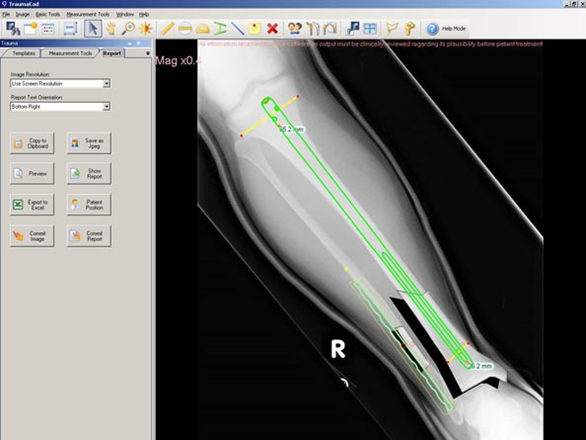
\includegraphics[width=.55\columnwidth]{images/trauma_cads.png}
	\caption{Colocaci\'on de un implante dentro de la aplicaci\'on TraumaCAD de OrthoCrat Ltd. \cite{REF_TRAUMA}}
	\label{fig:trauma_cads}
\end{figure}

En muchas ocasiones, es necesario moldear el implante tal que sea anat\'omicamente correcto y se adapte a una secci\'on del cuerpo. Este moldeado del implante consiste en un doblado que se realiza durante la operaci\'on, dentro del quir\'ofano. El doblado se aplica empleando una fuerza mec\'anica con una pinza especial. Cabe destacar que dichos sistemas no aplican deformaciones a sus plantillas ya que son est\'aticas, presentadas como un repositorio de im\'agenes.

En el siguiente cap\'itulo, se presenta un esquema general para los sistemas CAOS en la realizaci\'on de la planificaci\'on preoperatoria digital, incluyendo funcionalidades adicionales no existentes dentro de los sistemas mencionados anteriormente.
		%%%%%%%%%%%%%%%%%%%%%%%%%%%%%%%%%%%%%%%%%%
\chapter{Esquema CAOS propuesto}

En este cap\'itulo se presenta un esquema para la planificaci\'on preoperatoria digital en el \'area de Traumatolog\'ia. El esquema planteado fue presentado como un reporte t\'ecnico dentro de la Escuela de Computaci\'on de la Universidad Central de Venezuela, ver \cite{RAM09}. Posteriormente, se mejoro el trabajo mencionado anteriormente y fue enviado a una Conferencia Internacional \cite{RAM10}. A continuaci\'on se describe en detalle cada uno de los pasos aplicados a nuestra propuesta.

%%%%%%%%%%%%%%%%%%%%%%%%%%%%%%%%%%%%%%%%%%
\section{Propuesta}

En la Figura \ref{fig:esquema} se plantea un esquema general para los sistemas de planificaci\'on preoperatoria en el \'area de Traumatolog\'ia. Dicho esquema se puede resumir en siete etapas y algunos m\'odulos adicionales que complementan la funcionalidad del esquema. 
\begin{figure}[htb]
	\centering
	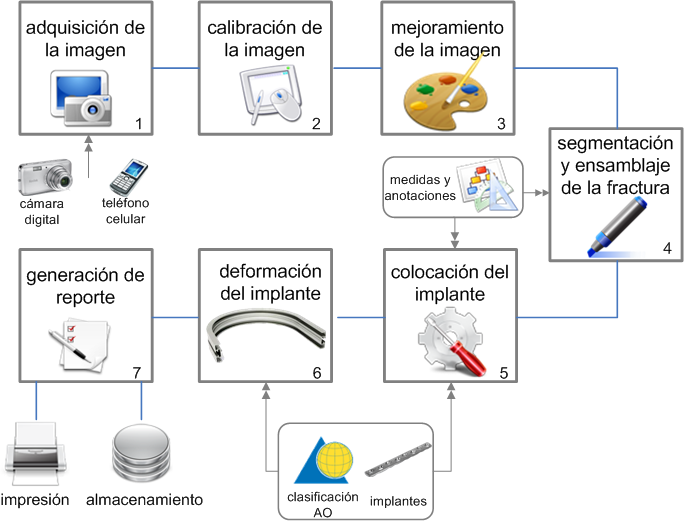
\includegraphics[width=.8\columnwidth]{images/esquema_tesis_mscv4.png}
	\caption{Esquema general de la planificaci\'on preoperatoria digital en Ortopedia}
	\label{fig:esquema}
\end{figure}

El sistema recibe como entrada una imagen correspondiente a una fractura de un paciente, la cual proviene de una placa radiogr\'afica. Una vez adquirida la imagen, se procede a un proceso de calibraci\'on para obtener medidas aproximadas de las proporciones dentro de la imagen (e.g. longitud del hueso en $mm.$). A la imagen calibrada se le puede aplicar t\'ecnicas de mejoramiento como aumento del brillo, contraste, etc., con el objetivo de ayudar en la extracci\'on de los fragmentos de una fractura por parte del traumat\'ologo. Una vez que el traumat\'ologo haya separado los fragmentos de huesos, efect\'ua el ensamblaje del hueso afectado como parte del procedimiento de planificaci\'on.

La fractura tratada puede requerir de un dispositivo externo (placa, tornillo, implante, etc.) para la reducci\'on del hueso. Dicho dispositivo ser\'a seleccionado de un conjunto de plantillas asociadas al tipo de fractura a tratar. Una vez colocado el dispositivo externo, el sistema permite al radi\'ologo aplicar deformaciones dependiendo de la anatom\'ia de la reducci\'on. Al finalizar los pasos antes mencionados, se obtiene el calco necesario para la cirug\'ia y la posibilidad de obtener un reporte con los datos tanto del paciente como del procedimiento a efectuar y su respectivo almacenamiento como parte de la historia cl\'inica del paciente.

Cada uno de los pasos de la Figura \ref{fig:esquema} son explicados con detalle en las secciones a continuaci\'on:

%%%%%%%%%%%%%%%%%%%%%%%%%%%%%%%%%%%%%%%%%%
\subsection{Adquisici\'on de la imagen}

En el modelo propuesto, las im\'agenes se obtienen empleando una c\'amara digital. El procedimiento consiste en los siguientes pasos:
\begin{enumerate}
	\item El m\'edico coloca sobre un negatoscopio la(s) placa(s) de Rayos-X para generar el contraste adecuado.
	\item Se procede a tomar la fotograf\'ia de la placa.
	\item Se descarga la imagen (en formato JPG, BMP, PNG o GIF) al computador.
\end{enumerate}
En la Figura \ref{fig:adquisicion} se ilustra la manera en que debe ser tomada una fotograf\'ia de una placa de Rayos-X. La c\'amara se coloca a una distancia de 1 m. $\pm$ 10 cm. de manera frontal tal que el \'angulo de visi\'on formado por la c\'amara ocupe toda la placa.
\begin{figure}[htb]
	\centering
	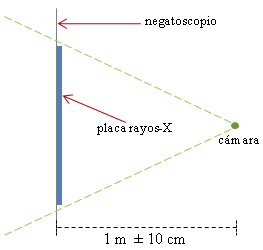
\includegraphics[width=0.4\columnwidth]{images/distancia_ch4.png}
	\caption{Esquema de adquisici\'on de la imagen empleando una c\'amara digital sobre la placa de Rayos-X colocada sobre un negatoscopio}
	\label{fig:adquisicion}
\end{figure}

La resoluci\'on de la fotograf\'ia debe ser de al menos $800 \times 600$ p\'ixeles. Para obtener la resoluci\'on m\'inima requerida de $800 \times 600$, se precisa de una c\'amara de al menos 0.5 megap\'ixeles. N\'otese que la resoluci�n en p\'ixeles cambia de una c\'amara a otra, de acuerdo a su capacidad de captura. Por ejemplo, al tomar una fotograf\'ia de una placa de un f\'emur de un infante se puede obtener la imagen a una resoluci\'on de $1024 \times 768$ p\'ixeles, pero al utilizar una c\'amara distinta y tomar la fotograf\'ia sobre la misma placa se puede obtener una resoluci\'on de $1680 \times 1050$ p\'ixeles.

Conocer las dimensiones reales de una imagen es relevante ya que permitir\'a realizar medidas sobre la misma. Las medidas realizadas sobre la anatom\'ia de un paciente permiten obtener las dimensiones reales de los segmentos de una fractura, la longitud de los huesos, el \'angulo formado entre dos secciones, etc. En la pr\'oxima secci\'on, se muestran los pasos necesarios para permitir la conversi\'on de p\'ixeles a mil\'imetros de la imagen de estudio en un proceso llamado calibraci\'on de la imagen.

%%%%%%%%%%%%%%%%%%%%%%%%%%%%%%%%%%%%%%%%%%
\subsection{Calibraci\'on de la imagen}

La calibraci\'on de la imagen consiste en realizar la correspondencia p\'ixel-mil\'imetro y de esta manera poder realizar medidas sobre la imagen a trabajar en la planificaci\'on. Una soluci\'on com\'un para la calibraci\'on en procesos donde se digitalizan placas de Rayos-X, es la introducci\'on de un objeto de tama\~no conocido al momento de la adquisici\'on de la misma (OR - Objeto de Referencia). Entonces, el proceso de calibraci\'on consiste en definir un Objeto de Referencia que sea utilizado en todos los casos de adquisici\'on de la imagen. Con el OR, se puede calcular un factor de correspondencia p\'ixel-mil\'imetro el cual se utilizar\'a para realizar las medidas correspondientes. En la presente secci\'on se muestran los pasos para la ejecuci\'on de esta etapa.

%%%%%%%%%%%%%%%%%%%%%%%%%%%%%%%%%%%%%%%%%%
\subsubsection{Preparaci\'on de la imagen}

En el esquema propuesto, se utiliz\'o como Objeto de Referencia una perforadora de papel, v\'ease la Figura \ref{fig:paper-punch}. La elecci\'on de este dispositivo de oficina se bas\'o en la necesidad de utilizar un OR que sea disponible en todo momento y pueda estar presente en el momento de la toma independientemente del negatoscopio a utilizar (e.g. negatoscopio general, port\'atil, de mural, etc.).
\begin{figure}[htb]
	\centering
		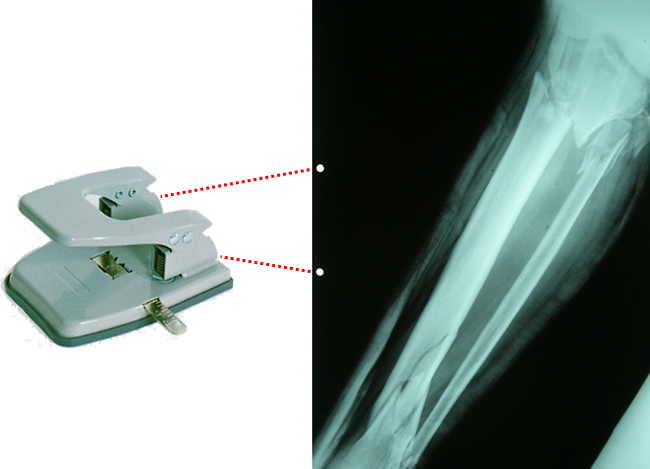
\includegraphics[width=0.4\columnwidth]{images/paperpunch.png}
	\label{fig:paper-punch}
	\caption{Perforadora de papel para crear los orificios en una placa de Rayos-X}
\end{figure}

Dado que la perforadora de papel siempre crea los orificios en los bordes de la placa, solamente se consideran las franjas dentro de la placa donde posiblemente se encuentren \'estas. Entonces, por cada imagen se extraen cuatro (4) subim\'agenes, como se observa en la Figura \ref{fig:paperholes}, para ser analizadas y encontrar los orificios: la parte superior, inferior, derecha e izquierda de la imagen. Para el caso de las subim\'agenes superior e inferior, el ancho corresponde al ancho de la imagen y el alto es de $10\%$ del alto de la imagen original. Se procede de manera similar para las subim\'agenes derecha e izquierda.
\begin{figure}[htb]
	\centering
		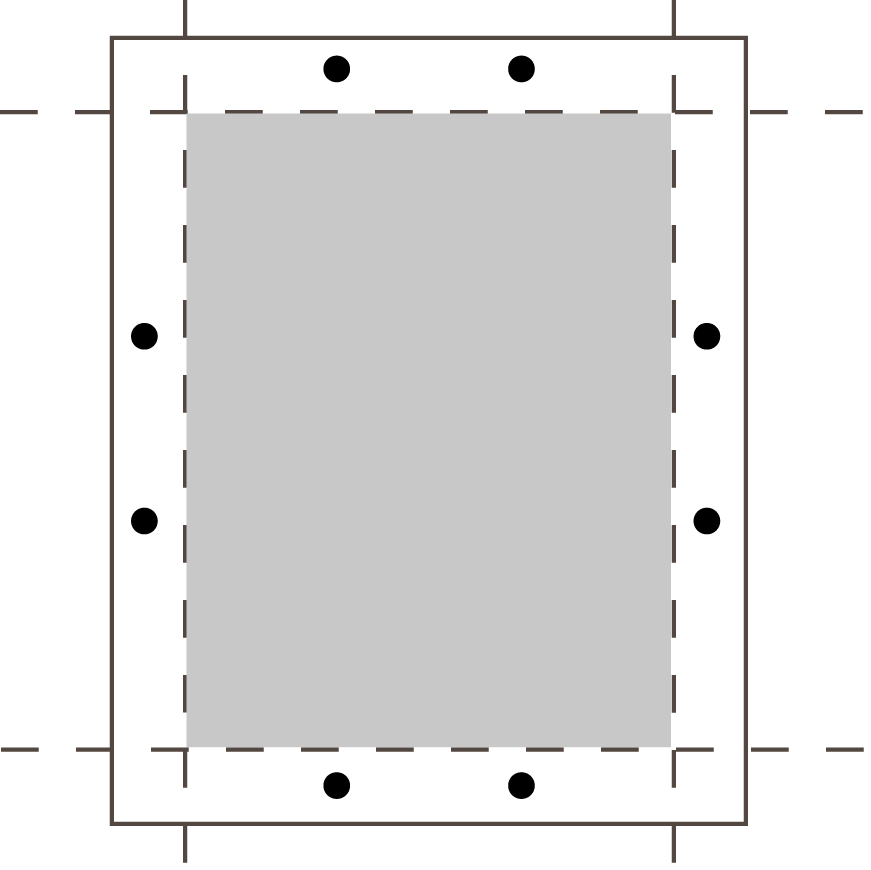
\includegraphics[width=0.4\columnwidth]{images/paperholes.png}	
	\caption{Cuatro (4) posibles franjas donde se abren los orificios con la perforadora de papel}
	\label{fig:paperholes}
\end{figure}

Para cada una de las subim\'agenes, se ejecuta el Algoritmo de B\'usqueda de Orificios y luego el proceso de Calibraci\'on. A continuaci\'on, se explica dicho algoritmo.

%%%%%%%%%%%%%%%%%%%%%%%%%%%%%%%%%%%%%%%%%%
\subsubsection{Algoritmo de B\'usqueda de Orificios} \label{AlgBusqOri1}

El Algoritmo de B\'usqueda de Orificios permite dada una Imagen $I$ de entrada, dos umbrales $U,T$ y un valor de error $E$, determinar la ubicaci\'on de los dos orificios, creados por la perforadora de papel, dentro de $I$. Cabe destacar que el algoritmo requiere como entrada una imagen binaria, es decir, que utilice un solo bit por p\'ixel en su representaci\'on. De esta forma solo existen dos colores: blanco y negro. Se asume que los c\'irculos a buscar ser\'an de color blanco por el contraste generado por el negatoscopio con la placa. Para obtener la imagen binaria, se realiza un proceso de segmentaci\'on a dos niveles de $I$ (\textit{image binarization}). Luego de la binarizaci\'on el algoritmo busca una serie de candidatos a c\'irculos que son colocados en una cola de prioridad bajo un criterio de similitud. Seguidamente, los elementos de la cola son extra\'idos y comparados entre s\'i para encontrar los de mayor similitud entre s\'i.

%%%%%%%%%%%%%%%%%%%%%%%%%%%%%%%%%%%%%%%%%%
\paragraph{Segmentaci\'on a dos niveles}

Con la segmentaci\'on a dos niveles, dada una imagen $I$ se quiere transformar $I$ en una nueva imagen con solo dos colores (e.g. blanco y negro). En el esquema propuesto, la imagen de entrada es a color, como se muestra en la Figura \ref{fig:segBW1}. Esta imagen es convertida a una imagen de 8-bits con paleta de colores, como se observa en la Figura \ref{fig:segBW2}.
\begin{figure}[htb]
  \begin{center} 
  \subfigure[]{\label{fig:segBW1}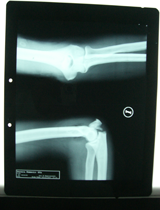
\includegraphics[width=0.30\columnwidth]{images/segmentationBW1.png}} \hspace{0.3cm} 	\subfigure[]{\label{fig:segBW2}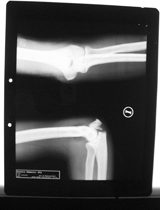
\includegraphics[width=0.30\columnwidth]{images/segmentationBW2.png}} \hspace{0.3cm}
  \subfigure[]{\label{fig:segBW3}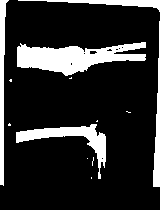
\includegraphics[width=0.30\columnwidth]{images/segmentationBW3.png}}
  \end{center}
  \caption{Etapas de conversi\'on de la imagen original a solo dos niveles de color. (a) Imagen RGB (b) Imagen en niveles de grises (c) Imagen binaria}
  \label{fig:segmentation}
\end{figure}

La conversi\'on de una imagen a color a una imagen a escala de grises se realiza empleando la Ec. \ref{eq:togray}, bajo el criterio explicado en \cite{UMB05}. Con esta ecuaci\'on se obtiene un valor $color_{gray}$ para cada p\'ixel, que representa la intensidad del p\'ixel (dentro del rango $0-255$), bas\'andose en la informaci\'on de cada banda de color de dicho p\'ixel en la imagen original: rojo ($R$), verde ($G$) y azul ($B$).
\begin{equation}
	\label{eq:togray}
	color_{gray} = 0.299 \times R + 0.587 \times G + 0.114 \times B
\end{equation}

Finalmente para obtener la imagen binaria $I_b$, como se muestra en la Figura \ref{fig:segBW3}, se realiza una umbralizaci\'on simple sobre el rango $[200-220]$. El valor adecuado dentro de ese rango, se selecciona de acuerdo a la proporci\'on del color negro en la imagen. Dicho rango fue seleccionado por ser satisfactorio sobre diversas im\'agenes de prueba.

%%%%%%%%%%%%%%%%%%%%%%%%%%%%%%%%%%%%%%%%%%
\paragraph{Algoritmo} \label{AlgBusqOri2}

Una vez obtenido $I_b$ se procede a realizar la b\'usqueda de los orificios. Los orificios creados por la perforadora de papel est\'an aproximadamente a la misma distancia del borde de la placa, es decir, un orificio se encuentra en el mismo sentido vertical u horizontal del otro. Este aspecto es importante al momento de determinar la similitud entre dos posibles orificios detectados por el algoritmo.

El algoritmo de B\'usqueda de Orificios, mostrado en el Algoritmo \ref{busqueda}, selecciona una serie de candidatos a c\'irculos y los coloca en una cola de prioridad. Los candidatos son seleccionados por la similitud entre s\'i para luego seleccionar los candidatos m\'as similares entre s\'i y de esa forma obtener los orificios.

\begin{algorithm}[htbp]
	\caption{B\'usqueda de Orificios}\label{busqueda}
	\begin{algorithmic}[1]
	\Procedure{FindCircles}{$I_b,U,T,E$}	\label{prototype}\Comment{$I_b$ = imagen; U,T = umbral; E = error permitido}
		\For {cada fila $F$ en $I_b$}	\label{first_for}
			\For {cada p\'ixel $P(x,f)$ de color blanco en $F$}
				\State $pN \gets pS \gets pE \gets pO \gets 0$	\Comment{\# de p\'ixeles blancos en direcci\'on Norte, Sur, Este y Oeste}
				\Loop
					\If{$P(x,f+1) = blanco$}
						$pN \gets pN + 1$
					\EndIf
					\If{$P(x,f-1) = blanco$}
						$pS \gets pS + 1$
					\EndIf
					\If{$P(x+1,f) = blanco$}
						$pE \gets pE + 1$
					\EndIf
					\If{$P(x-1,f) = blanco$}
						$pO \gets pO + 1$
					\EndIf
				\EndLoop
				\If{$p\{N|S|E|O\} > 0$ \underline{y} $|((pN+pS)/2) - ((pE+pO)/2)| < U$}
					\State $d_1 = |pS - pN|$
					\State $d_2 = |pE - pO|$
					\If{$|d_1 - d_2| \le T$}
					\Comment{posiblemente $P(x,f)$ es el centro de un c\'irculo}
						\State $Mask \gets \Call{CreateMask}{(pN+pS)/2}$
						\State $error \gets \Call{ECM}{Mask, I_b, P(x,f)}$
							\If{$error \le E$}
								\State $Priority\_Queue.Add(P(x,f), (pN+pS)/2)$
							\EndIf
					\EndIf
				\EndIf
			\EndFor
		\EndFor
		\State $C_1,C_2 \gets \Call {Find2MostSimilar}{Priority\_Queue}$
	\State \textbf{return} $C_1,C_2$\Comment{$C_1$ y  $C_2$ son los orificios hechos por la perforadora}
	\EndProcedure
	\end{algorithmic}
\end{algorithm}

El algoritmo empieza recorriendo cada p\'ixel de color blanco de cada fila de la subimagen que contiene al candidato, con el objetivo de determinar cu\'al es la distancia hasta los bordes de ese posible candidato. Con estos valores, la idea es determinar cu\'al de \'estos es sim\'etrico con respecto a un p\'ixel centro de c\'irculo. Se puede observar que la Figura \ref{fig:circles1} es m\'as irregular en proporci\'on a la distancia a sus bordes desde el centro que la Figura \ref{fig:circles2}. Cabe destacar, que la Figura \ref{fig:circles1} no entra como candidato de orificio en el algoritmo.
\begin{figure}[htb]
  \begin{center} \subfigure[]{\label{fig:circles1}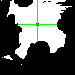
\includegraphics[width=0.20\columnwidth]{images/circles1.png}} \hspace{1.1cm} \subfigure[]{\label{fig:circles2}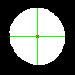
\includegraphics[width=0.20\columnwidth]{images/circles2.png}}
  \end{center}
  \caption{Recorrido en cuatro direcciones para una posici\'on $(x,y)$ de un posible candidato. (a) Forma irregular (b) Forma de orificio}
  \label{fig:circles}
\end{figure}

Para determinar el factor de simetr\'ia de un candidato, se verifica si la distancia desde el centro hacia las cuatro direcciones cardinales tienen longitudes similares. Estas distancias son almacenadas en las variables $pN,pS,pE,pO$ que se muestran en el Algoritmo de B\'usqueda de Orificios y se pueden observar en la Figura \ref{fig:circulo}. 
\begin{figure}[htb]
	\centering
		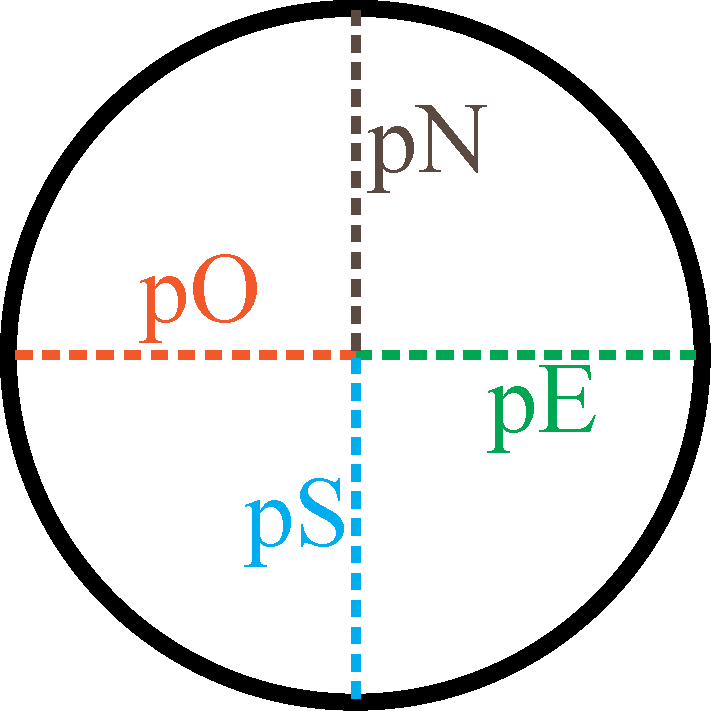
\includegraphics[width=0.25\columnwidth]{images/circle.png}
	\caption{Posible candidato a c\'irculo donde se identifican las 4 distancias obtenidas desde el centro del mismo.}
	\label{fig:circulo}
\end{figure}

Al realizar est\'a operaci\'on en cada p\'ixel de cada fila, permite que se utilicen los valores antes mencionados para el siguiente p\'ixel a analizar. Por ejemplo, si estamos en la posici\'on $(x,y)$ al avanzar a la posici\'on $(x+1,y)$ es ideal utilizar los valores $pN,pS,pE,pO$ de $(x,y)$ para no calcularlos nuevamente.

Para ello se construye una estructura de datos que consiste en un arreglo del tama\~no de una fila donde cada celda almacena 4 valores: $pN,pS,pE,pO$. Con esta estructura, para los valores $pE,pO$ de una posici\'on $(x,y)$ se utilizan sus adyacentes. Cuando se recorre una fila nueva, es decir, la fila $(x,y+1)$, los valores $pN,pS$ son copiados como valores iniciales si existe un p\'ixel blanco en esa posici\'on con el objetivo de no contarlos nuevamente.

Con los valores $pN,pS,pE,pO$ es posible determinar si una posici\'on $(x,y)$ es el centro de un candidato a orificio basados en los valores de umbral $U,T$. El valor umbral $U$ es la diferencia permitida entre el alto y el ancho promediado de un candidato. Dicho valor va a permitir descartar candidatos que su eje vertical/horizontal sea muy distinto al eje contrario. Es por ello que la verificaci\'on dentro del Algoritmo \ref{busqueda} se hace como $\frac{pN+pS}{2} - \frac{pO+pE}{2} < U$. El valor umbral $T$ es la diferencia entre la longitud de los di\'ametros de un posible candidato en forma de c\'irculo. El valor ideal de esta diferencia, debe ser $0$. Este valor permite discriminar candidatos que sean muy ovalados y filtrar los que sean m\'as redondos.

Luego, se invoca a la funci\'on \verb+CreateMask+ donde se construye un arreglo bidimensional que contiene blancos y negros, donde los p\'ixeles blancos forman un c\'irculo, con el objetivo de hacer una coincidencia de patrones \cite{PAJ01} (\textit{pattern matching}) de un espacio dentro de la imagen con un c\'irculo perfecto.

Al realizar la coincidencia de patrones, se calcula el error cuadr\'atico medio \cite{LEH98} con la funci\'on \verb+ECM+. Dicho valor de error permite determinar qu\'e tan parecido es un posible candidato a un c\'irculo perfecto. Si el valor de este error es inferior a cierto umbral $E$, entonces es considerado como un candidato potencial. En las pruebas realizadas, se tomo como valor $E$ un $12\%$ de discrepancia ya que permite considerar los casos en donde la imagen de entrada no sea de buena calidad. Posteriormente, dicha posici\'on $(x,y)$ con un radio de dimensi\'on $(pN+pS)/2$ es insertada en una cola de prioridad. En dicha cola la mayor prioridad la tiene el candidato con menor error $E$.

Como \'ultimo paso del algoritmo, se invoca a la funci\'on \verb+Find2MostSimilar+ que recibe como par\'ametro a la cola de prioridad y busca el par de candidatos de mayor similitud. Los criterios para decidir la similitud son:
\begin{itemize}
	\item Si el candidato $C_1$ ocupa un \'area $A_1$ en p\'ixeles, entonces el candidato $C_2$ tendr\'a una \'area $A_2$ en el rango $A_1 - (0.2*A_1) \le A_2 \le A_1 + (0.2*A_1)$.
	\item Si un candidato se encuentra a una distancia $dx$ del borde de la imagen, el otro candidato debe estar a una distancia $d \le dx*1.5$ del mismo borde.
	\item La distancia entre ambos candidatos, debe ser mayor al $15\%$ del total del lado donde se encuentran (lado horizontal o lado vertical) en la imagen.
\end{itemize}

Finalmente, es posible haber obtenido un solo orificio, dos orificios \'o ninguno. En caso de no haber obtenido ning\'un orificio o solamente uno, se provee la opci\'on de seleccionar el(los) orificio(s) faltante(s) de forma manual. En el caso de haber encontrado ambos orificios, se procede a la calibraci\'on.

%%%%%%%%%%%%%%%%%%%%%%%%%%%%%%%%%%%%%%%%%%
\paragraph{Correspondencia}

Una vez obtenidos ambos orificios, el proceso de calibraci\'on es trivial. Seg\'un el est\'andar ISO (\textit{International Organization for Standardization}) 838 \cite{REF_ISO838} publicado en 1974, titulado ``\textit{Paper $--$ Holes for general filing purposes}'', la distancia entre los centros de cada orificio tiene una medida de $80 \pm 0.5 mm$.

Utilizando el est\'andar, es posible definir est\'a medida como la calibraci\'on para cualquier imagen. Si la distancia entre los centros de los orificios corresponde a $p$ p\'ixeles, entonces $p = 80mm$. Entonces, un p\'ixel corresponde a $\frac{80}{p} mm$. Existen fabricantes de perforadores de orificios que no utilizan el est\'andar ISO en la fabricaci\'on de los mismos y este hecho ocasionar\'ia una calibraci\'on incorrecta. Una soluci\'on a este problema, es ofrecer la posibilidad de modificar la distancia entre orificios de acuerdo al perforador de papel que se utilice, por ejemplo $79.5mm.$, $75mm.$, $81mm.$, etc.

%%%%%%%%%%%%%%%%%%%%%%%%%%%%%%%%%%%%%%%%%%
\subsection{Mejoramiento de la imagen}

Una vez calibrada la imagen, el m\'edico radi\'ologo tiene la posibilidad de modificar ciertos valores visuales dentro de la imagen para mejorar la calidad visual de la misma. Dado que las im\'agenes son de 8-bit, esto permite crear un histograma de frecuencias en el rango de valores $[0-255]$. Dentro de ese rango se pueden definir dos caracter\'isticas empleadas para el mejoramiento: Ventana (\textit{window}) y Nivel (\textit{level}). El \textit{window} define el tama\~no de un rango de valores consecutivos dentro del histograma. El \textit{level} define un valor dentro del rango de valores de la imagen. Con estos valores, es posible definir el valor m\'inimo y m\'aximo de p\'ixel de un rango de datos, al que llamaremos ``ventana''. Si $V_{max}$ define el valor m\'aximo y $V_{min}$ el m\'inimo, entonces $V_{min}=level - \frac{window}{2}$ y $V_{max}=level + \frac{window}{2}$. En la Fig. \ref{fig:window} se muestra un histograma donde se indica el ancho de la ventana demarcado por unas l\'ineas punteadas.
\begin{figure}[htbp]
	\centering
	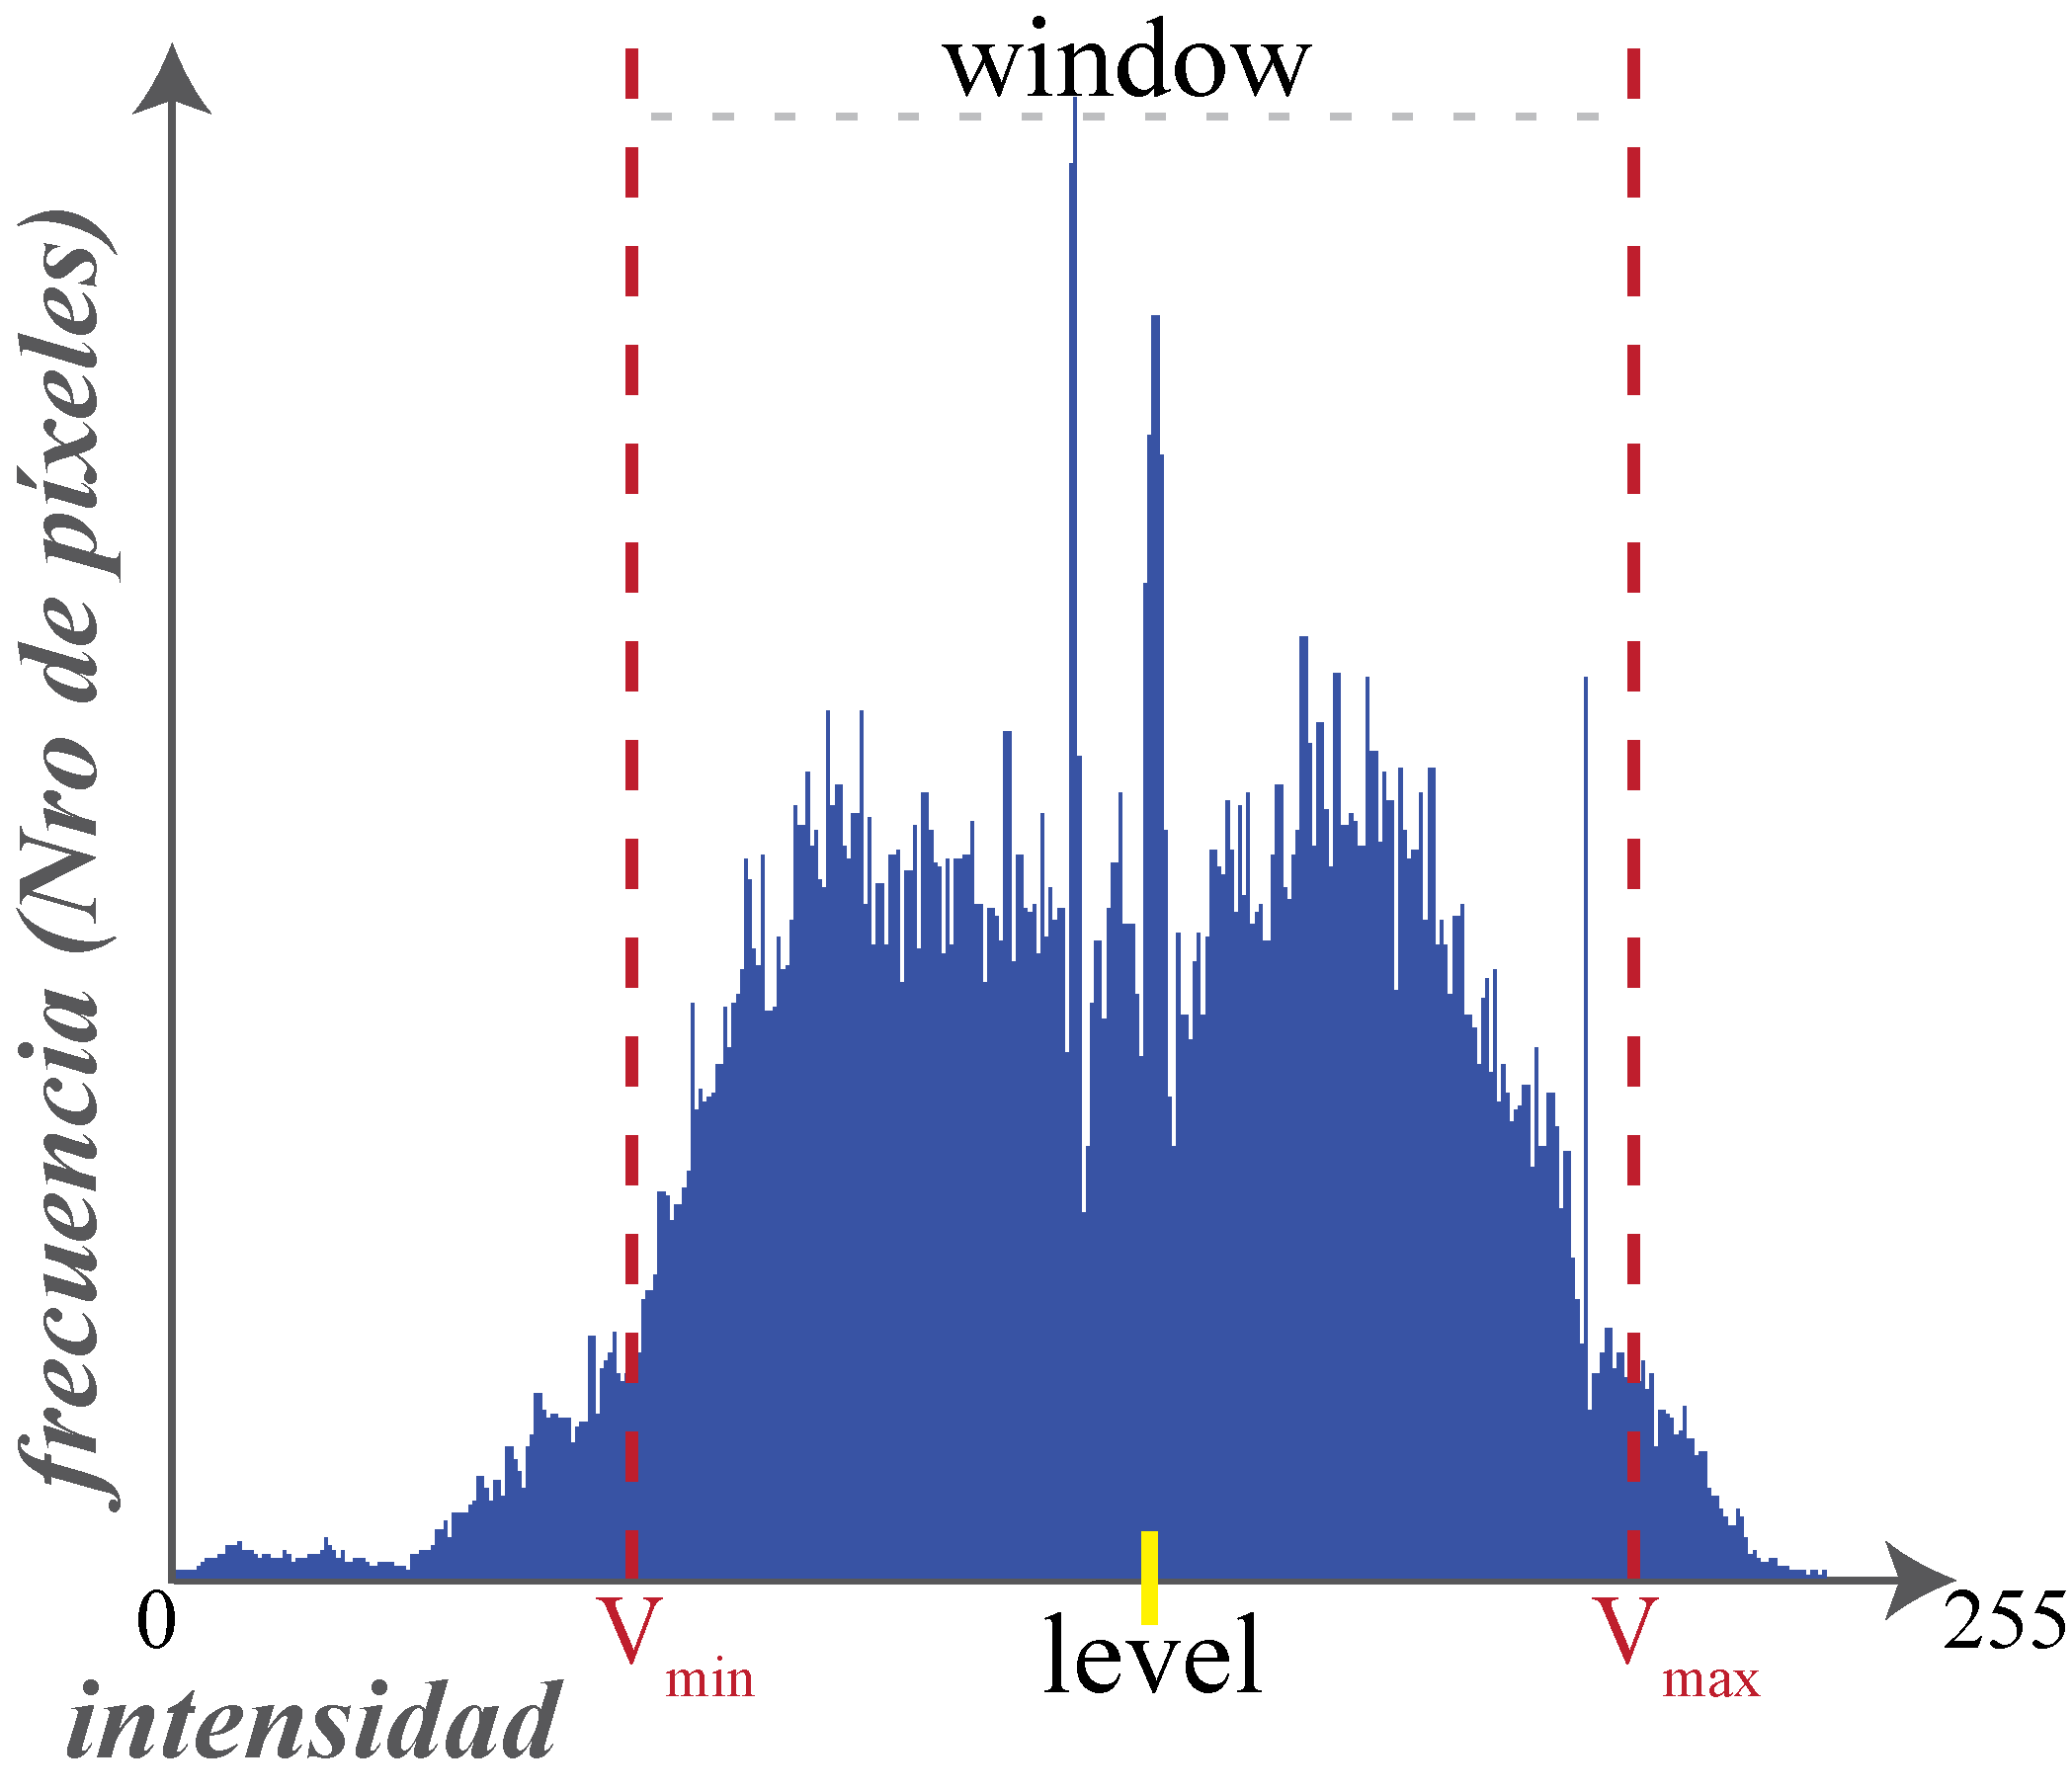
\includegraphics[width=0.5\columnwidth]{images/histograma.png}
	\caption{Histograma de intensidades que muestra el \textit{window} y \textit{level} dentro del histograma.}
	\label{fig:window}
\end{figure}

Por defecto, los valores de \textit{window} y \textit{level} son $255$ y $128$ respectivamente, para que la ventana ocupe todo el rango de valores de la imagen. Sin embargo, ajustando los valores de \textit{window} y \textit{level}, se puede modificar el contraste de la imagen. Por ejemplo, al definir el valor $W = 200$ y $L = 110$, todos los p\'ixeles con una intensidad $I \le 10$ ser\'an llevados a 0, y todos los p\'ixeles con una intensidad $I \ge 210$ ser\'an llevados a 255. Los p\'ixeles con intensidades entre $10$ y $210$ ser\'an mapeados linealmente al rango de valores de salida, que es de $[0,255]$.

En la Figura \ref{fig:mejoramiento1} se muestra una imagen adquirida de un estudio de un paciente luego de ser calibrada. En la Figura \ref{fig:mejoramiento2} se muestra la misma imagen pero con valores de \textit{window} $W=100$ y \textit{level} $L=128$. Por otra parte, en la Figura \ref{fig:mejoramiento3} se tienen los valores $W=255$ y $L=240$. El m\'edico es el encargado de manipular estos valores con el objetivo de obtener un mejor contraste en la imagen para poder realizar la reducci\'on de la fractura en la planificaci\'on.
\begin{figure}[htbp]
  \begin{center}
    \subfigure[]{\label{fig:mejoramiento1}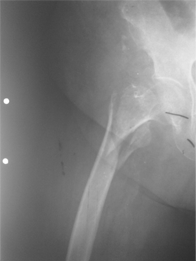
\includegraphics[width=0.30\columnwidth]{images/mejoramiento1.png}} \hspace{0.4cm} \subfigure[]{\label{fig:mejoramiento2}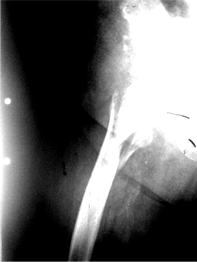
\includegraphics[width=0.30\columnwidth]{images/mejoramiento2.png}} \hspace{0.4cm}  \subfigure[]{\label{fig:mejoramiento3}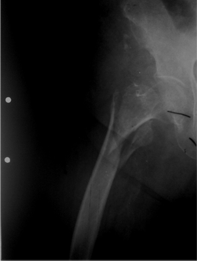
\includegraphics[width=0.30\columnwidth]{images/mejoramiento3.png}}
  \end{center}
  \caption{Mejoramiento de la imagen con diversos valores de \textit{window} y \textit{level} (a) $W=255$ y $L=128$ (b) $W=100$ y $L=128$ (c) $W=255$ y $L=240$}
  \label{fig:mejoramiento}
\end{figure}

Adicionalmente, se ofrece una opci\'on sugerida de contraste basado en la cantidad de intensidades presentes en la imagen. Dicha opci\'on consiste en asignar valores de \textit{window} y \textit{level} tal que la imagen muestre valores relevantes en el contraste adecuado. Para ello se calcula de intensidad promedio de la imagen $I_{average}$. Al mismo tiempo, se calcula el valor de $N_p$ que representa el n\'umero de p\'ixeles que est\'an por encima de $I_{average}$. Finalmente se ubica el valor de \textit{level} en el valor medio del rango de intensidades de la imagen y el valor del \textit{window} es $N_p$.

%%%%%%%%%%%%%%%%%%%%%%%%%%%%%%%%%%%%%%%%%%
\subsection{Segmentaci\'on y ensamblaje de la fractura}

Para efectuar la reducci\'on de una fractura se requiere extraer los fragmentos de hueso presente. Una vez seleccionados los fragmentos, el traumat\'ologo debe ensamblarlos y colocarlos en sus posiciones correctas y as\'i completar la reducci\'on de la fractura.

La selecci\'on de los fragmentos de la fractura en la imagen, requiere un proceso de segmentaci\'on \cite{UMB05} donde se separen dichos fragmentos del hueso a tratar. Los algoritmos existentes para la segmentaci\'on autom\'atica de im\'agenes de Rayos-X no son triviales ya que no existe un procedimiento est\'andar para su ejecuci\'on. En la literatura existen diversas t\'ecnicas para la segmentaci\'on de im\'agenes m\'edicas \cite{HARA85,PAL93,PHAM00} entre las que destacan: los modelos deformables \cite{KASS88,TER87,TER88}, las plantillas deformables param\'etricas \cite{YUI92}, los modelos de distribuci\'on de puntos \cite{COOT94}, las plantillas gr\'aficas \cite{AMIT96} y las plantillas basadas en esqueletos \cite{PIZ98,PIZ99}, entre otras t\'ecnicas. Dichas t\'ecnicas no son 100\% efectivas para todas las im\'agenes. Para conseguir una segmentaci\'on adecuada por lo general se emplean varias de \'estas t\'ecnicas y/o se aplican modificaciones acorde a la imagen en cuesti\'on.

Otra forma de extracci\'on de fragmentos es emplear la segmentaci\'on manual, la cual consiste en delinear los bordes de los fragmentos e ir construyendo un pol\'igono que encierre el fragmento de hueso, como se observa en la Figura \ref{fig:fragmentation}.
\begin{figure}[htb]
  \begin{center} \subfigure[]{\label{fig:segmentation1}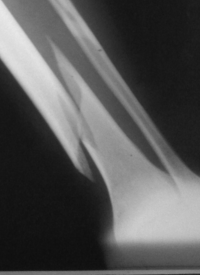
\includegraphics[width=0.25\columnwidth]{images/segmentation1.png}} \hspace{0.5cm} \subfigure[]{\label{fig:segmentation2}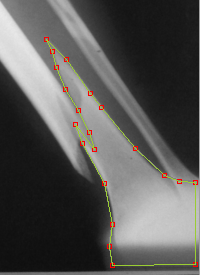
\includegraphics[width=0.25\columnwidth]{images/segmentation2.png}}\hspace{0.5cm} \subfigure[]{\label{fig:segmentation3}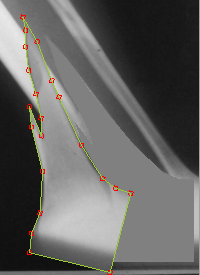
\includegraphics[width=0.25\columnwidth]{images/segmentation3.png}} \hspace{0.5cm}
  \end{center}
  \caption{Segmentaci\'on manual de una fractura donde se seleccionan los fragmentos de hueso para ser colocados en su posici\'on correcta. (a) Fractura simple (b) Pol\'igono que delimita la secci\'on a segmentar (c) Pol\'igono despu\'es de aplicar rotaciones y traslaciones}
  \label{fig:fragmentation}
\end{figure}

En el esquema propuesto se opt\'o por una segmentaci\'on manual. En la Figura \ref{fig:segmentation1} se muestra una fractura simple a ser segmentada por el m\'edico radi\'ologo. En la Figura \ref{fig:segmentation2} se observa una serie de puntos gu\'ia (en color rojo) sobre el contorno del fragmento unidos por una l\'inea formando un pol\'igono irregular. Finalmente, es posible aplicar rotaciones y traslaciones sobre el fragmento con el objetivo de ser colocado en su posici\'on anat\'omicamente correcta para realizar la reducci\'on por parte del radi\'ologo, ver Figura \ref{fig:segmentation3}.

%%%%%%%%%%%%%%%%%%%%%%%%%%%%%%%%%%%%%%%%%%
\subsubsection{Medidas y anotaciones}

Una vez calibrada la imagen es posible realizar mediciones de la anatom\'ia en una imagen empleando diversas herramientas. Las mediciones dentro de una imagen de Rayos-X son importantes para el tratamiento de un paciente, ya que permiten obtener las dimensiones de los segmentos de una fractura, la longitud de los huesos y el \'angulo entre dos secciones (e.g. diferencia entre fragmentos de hueso en una fractura), entre otros. Las medidas son realizadas en $mm.$ y permiten al radi\'ologo definir dimensiones y longitudes \'utiles para su planificaci\'on antes de entrar al quir\'ofano.

Algunas de las herramientas de calibraci\'on se observan en la Figura \ref{fig:medidas}. La Figura \ref{fig:medida1} muestra un tipo de medida denominada \textit{Regla} que consiste en una l\'inea recta que une dos puntos, mostrando la medida en $mm.$ La herramienta denominada \textit{\'Angulo} permite determinar, en grados, el \'angulo existente entre un par de l\'ineas rectas con un punto en com\'un, como se observa en la Figura \ref{fig:medida2}. La \'ultima herramienta de medici\'on se denomina \textit{C\'irculo} y crea un c\'irculo definido por un centro y un di\'ametro, ver Figura \ref{fig:medida3}, la medida es en $mm.$ y viene dada por el valor de su di\'ametro.
\begin{figure}[htb]
  \begin{center}
    \subfigure[]{\label{fig:medida1}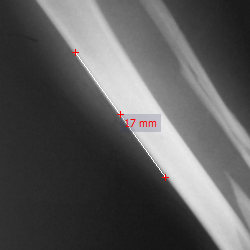
\includegraphics[width=0.35\columnwidth]{images/medirlinea.png}} \hspace{0.55cm} \subfigure[]{\label{fig:medida2}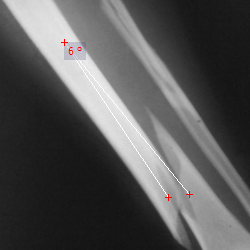
\includegraphics[width=0.35\columnwidth]{images/medirangulo.png}}\hspace{0.55cm}  \subfigure[]{\label{fig:medida3}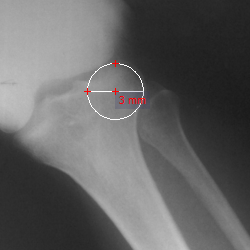
\includegraphics[width=0.35\columnwidth]{images/medircircle.png}} \hspace{0.55cm} \subfigure[]{\label{fig:medida4}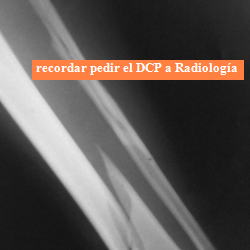
\includegraphics[width=0.35\columnwidth]{images/annotation.png}}
  \end{center}
  \caption{Herramientas de medidas y anotaciones. (a) Regla (b) \'Angulo (c) C\'irculo (d) Anotaci\'on}
  \label{fig:medidas}
\end{figure}

Una funcionalidad sumamente \'util dentro de la planificaci\'on de una operaci\'on son las anotaciones. Las anotaciones permiten colocar informaci\'on de inter\'es dentro de la imagen en formato de texto. Las notas colocadas dentro de la planificaci\'on son libres a juicio del m\'edico radi\'ologo. En la Figura \ref{fig:medida4} se observa un ejemplo de una anotaci\'on. Para facilidad del usuario es posible cambiar el tipo y tama\~no de letra as\'i como el color del fondo del mismo.

%%%%%%%%%%%%%%%%%%%%%%%%%%%%%%%%%%%%%%%%%%
\subsection{Colocaci\'on del implante} \label{IMPLANTE}

Un hueso fracturado debe ser cuidadosamente colocado en la posici\'on adecuada hasta que sea lo suficientemente fuerte como para soportar el peso del paciente, empleando alg\'un tipo de implante. Hasta el siglo pasado \cite{REF_AO}, los m\'edicos se basaron en emplear solamente yesos y f\'erulas para apoyar el hueso por fuera del cuerpo (fijaci\'on externa). Pero el desarrollo en el campo de la cirug\'ia redujo el riesgo de infecci\'on, permitiendo que los m\'edicos puedan trabajar directamente con el hueso y colocar implantes internos (fijaci\'on interna). 

Nuevos materiales tales como acero inoxidable, cobalto y titanio no son solo duraderos, sino que tambi\'en son lo suficientemente fuertes y flexibles para apoyar el hueso. Estos materiales tambi\'en son compatibles con el cuerpo y rara vez causan una reacci\'on al\'ergica en el paciente. Los tipos m\'as comunes de la fijaci\'on son: los alambres, placas, barras, clavijas, pines, clavos y tornillos.

Una vez que se obtienen los segmentos de hueso de una fractura y luego de haber aplicado la reducci\'on de la misma, es decisi\'on del traumat\'ologo la colocaci\'on y selecci\'on de implantes para realizar una fijaci\'on del hueso como parte del tratamiento quir\'urgico. Dependiendo del tipo de fractura, posici\'on anat\'omica y edad del paciente, entre otras variables, se procede a seleccionar el implante adecuado.

El esquema CAOS propuesto, plantea el uso de una librer\'ia \'o repositorio donde se almacenan los diversos implantes. Una librer\'ia de implantes es un conjunto de plantillas (\textit{templates}) de traumatolog\'ia clasificadas bajo alg\'un criterio. De esta forma, se selecciona un tipo de implante (e.g. clavo, placa, etc.), el material del que est\'a hecho y sus dimensiones (e.g. 12mm, 3.5 mm, etc.) para ser colocados en la planificaci\'on preoperatoria a construir.

Una base de datos es una forma de almacenamiento adecuada para colocar la gran cantidad de implantes requeridos para los sistemas CAOS de planificaci\'on preoperatoria. La librer\'ia de implantes utilizada en nuestra propuesta, se muestra como un \'arbol, ver Figura \ref{fig:arbol}, donde cada nivel de jerarqu\'ia indica un orden de acuerdo a la medida, material, tama\~no, etc.
\begin{figure}[htbp]
	\centering
	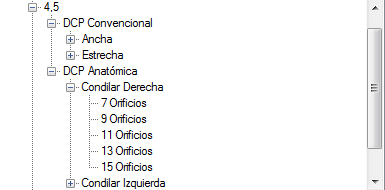
\includegraphics[width=0.5\columnwidth]{images/arbol.png}
	\caption{Vista en forma de \'arbol para representar los implantes de la librer\'ia}
	\label{fig:arbol}
\end{figure}

Una vez seleccionado el implante, \'este se extrae desde un archivo en formato STL (\textit{stereolithography}) generado por el \textit{software} Autodesk Inventor \cite{website:inventor}. En Autodesk Inventor se construye el implante a ser utilizado y es exportado en el formato STL que permite obtener una superficie 3D basada en tri\'angulos.

En el esquema propuesto, el implante seleccionado se muestra como se observa en la Figura \ref{fig:implantproj}, donde se debe seleccionar la orientaci\'on de la vista a utilizar y las dimensiones a emplear.
\begin{figure}[htbp]
	\centering
	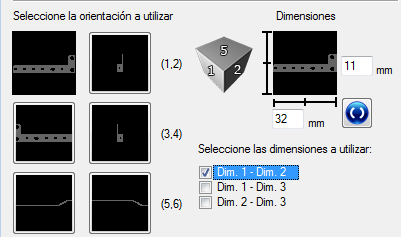
\includegraphics[width=0.60\textwidth]{images/implantprojection.png}
	\caption{Selecci\'on de los par\'ametros necesarios para colocar el implante en la planificaci\'on preoperatoria}
	\label{fig:implantproj}
\end{figure}

Dado que el implante se encuentra representado como una geometr\'ia en 3D, es necesario realizar el proceso de despliegue a 2D. Para ello, se aplica la proyecci\'on ortogonal que consiste en trazar rayos paralelos desde la posici\'on de la c\'amara en direcci\'on hacia el objeto de inter\'es. La posici\'on de la c\'amara se encuentra a una distancia infinita del objeto, resultando que los rayos de visi\'on sean paralelos al plano de proyecci\'on. Los puntos de intersecci\'on de los rayos con el plano de proyecci\'on corresponden al resultado esperado.
\begin{figure}[htbp]
	\centering
	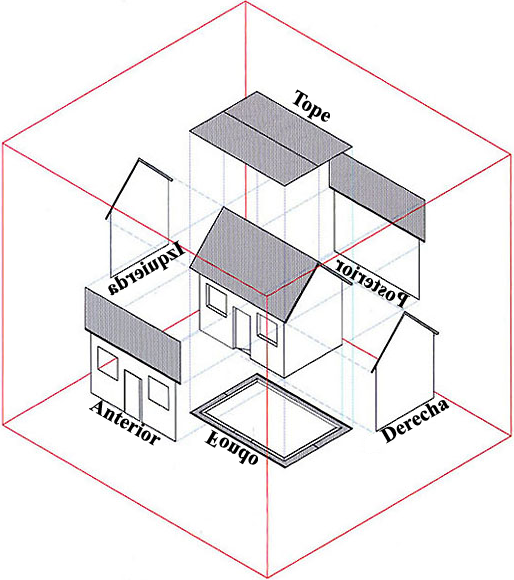
\includegraphics[width=0.35\textwidth]{images/house.png}
	\caption{Proyecci\'on paralela de un objeto casa sobre cada una de las caras de un cubo para obtener 6 proyecciones}
	\label{fig:house}
\end{figure}

En la Figura \ref{fig:house} se muestra un ejemplo de proyecci\'on paralela para un objeto que representa una casa, aplicada sobre cada cara de un cubo. Bajo este esquema, es posible obtener diferentes vistas para un objeto: tope, fondo, derecha, izquierda, anterior y posterior. Al seleccionar un implante en la interfaz propuesta, ver Figura \ref{fig:implantproj}, es posible seleccionar la vista a aplicar para una planificaci\'on. Las vistas se encuentran numeradas del 1 al 6 y adicionalmente se debe escoger las dimensiones a aplicar. Dado que no se conoce a priori la orientaci\'on original del implante (obtenido de Autodesk Inventor \cite{website:inventor}) se provee la opci\'on de seleccionar las dimensiones que representan las distancias que ocupa el implante (ancho, alto y profundidad).

%%%%%%%%%%%%%%%%%%%%%%%%%%%%%%%%%%%%%%%%%%
\subsection{Deformaci\'on del implante} \label{DEFO}

Como vimos anteriormente, los sistemas CAOS deben proveer una librer\'ia de implantes donde el m\'edico cirujano seleccione uno de \'estos para ser colocados en la fractura en cuesti\'on. En muchas ocasiones, es necesario moldear (deformar) el implante tal que sea anat\'omicamente correcto y se adapte al hueso fracturado. 

Dentro del quir\'ofano, el m\'edico cirujano emplea un alicate especial para el doblado de los implantes. En el sistema CAOS propuesto, la deformaci\'on del implante se realiza simulando la aplicaci\'on de una fuerza mec\'anica tal como se realiza en un quir\'ofano. 

En la Figura \ref{fig:tornillo}, se muestra un implante (placa) colocado sobre un f\'emur y su doblado dentro del mismo. Cabe destacar, que el doblado es una tarea exclusiva del m\'edico cirujano y no requiere mucha precisi\'on.
\begin{figure}[htb]
  \begin{center}
 \subfigure[]{\label{fig:tornillo1}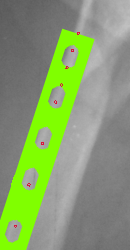
\includegraphics[width=0.23\columnwidth]{images/tornillo1.png}} \hspace{0.15cm} 			\subfigure[]{\label{fig:tornillo2}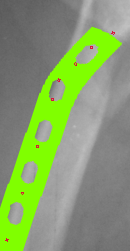
\includegraphics[width=0.23\columnwidth]{images/tornillo2.png}}
  \end{center}
  \caption{Implante de una placa de $4.5$ mm. de comprensi\'on convencional estrecha de 8 orificios sobre una placa de Rayos-X. (a) Sin aplicar deformaci\'on (b) Con una peque\~na deformaci\'on}
  \label{fig:tornillo}
\end{figure}

Tanto en el momento de la colocaci\'on del implante como en el de su deformaci\'on, es posible consultar en una gu\'ia de referencia los tipos de fracturas existentes seg\'un la clasificaci\'on AO. En el siguiente Cap\'itulo, se presentar\'a una descripci\'on m\'as detallada del proceso de deformaci\'on aplicado en nuestro trabajo.

%%%%%%%%%%%%%%%%%%%%%%%%%%%%%%%%%%%%%%%%%%
\subsubsection{Biblioteca de clasificaci\'on AO}

Una vez confirmada la fractura de un paciente, \'esta es localizada y clasificada de acuerdo a un esquema establecido. El esquema de clasificaci\'on de una fractura est\'a especificado de acuerdo a su ubicaci\'on anat\'omica. El esquema de clasificaci\'on utilizado en este trabajo es el AO \cite{REF_AO}.

En el esquema internacional de clasificaci\'on de fracturas AO, el m\'edico traumat\'ologo clasifica una fractura de acuerdo a la ubicaci\'on de la misma y sus caracter\'isticas morfol\'ogicas. AO plantea una clasificaci\'on basada en dos n\'umeros: el primero indica una ubicaci\'on en el cuerpo (1-h\'umero, 2-c\'ubito y radio, 3-f\'emur y 4-tibia y peron\'e) y el segundo, el segmento dentro del hueso (1-proximal, 2-diafisal, 3-distal). Una vez seleccionados ambos n\'umeros, entra en una clasificaci\'on por tipo de fractura (A-simple, B-en cu\~na, C-compleja). Luego, la fractura es dividida en tres grupos que miden la escala de severidad de la misma (1, 2, 3).

Esta clasificaci\'on es utilizada como una gu\'ia para el pron\'ostico y eficiencia en el tratamiento de una fractura. El esquema AO es recomendado internacionalmente porque es cl\'inicamente relevante, sencillo, reproducible y provee una buena estimaci\'on del resultado cl\'inico \cite{MULL90}. 

La biblioteca de referencia que nuestro sistema provee, ayudar\'a considerablemente al m\'edico radi\'ologo para que en cualquier momento pueda consultarla para una determinada fractura. En la Figura \ref{fig:aoexample} se observa la forma como se presenta la biblioteca de clasificaci\'on: a) se selecciona el hueso a estudiar y b) se selecciona la parte de la misma.
\begin{figure}[htbp]
  \begin{center}
    \subfigure[]{\label{fig:aoexample1}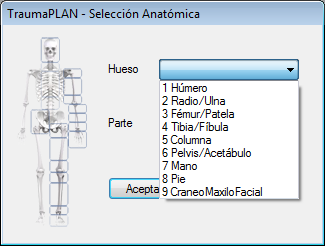
\includegraphics[width=0.45\columnwidth]{images/AOhueso.png}} \hspace{0.15cm} 			\subfigure[]{\label{fig:aoexample2}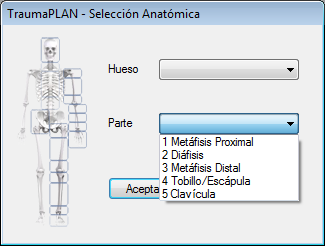
\includegraphics[width=0.45\columnwidth]{images/AOparte.png}}
  \end{center}
  \caption{Biblioteca de clasificaci\'on AO. (a) selecci\'on del hueso a consultar (b) parte dentro del hueso}
  \label{fig:aoexample}
\end{figure}

Una vez seleccionado el hueso y la parte, aparece el tipo de fractura y su severidad. Existe un m\'aximo de 9 clasificaciones posibles para ello, y son mostradas como im\'agenes para su mejor presentaci\'on. Para cada una de las clasificaciones mostradas, se tiene una imagen ejemplo de la fractura, una placa radiogr\'afica con la fractura y una peque\~na descripci\'on de la misma. En la Figura \ref{fig:aoexamplefinal} se puede observar las fracturas de f\'emur en la parte diafisiaria.
\begin{figure}[htbp]
	\centering
	\includegraphics[width=0.50\textwidth]{images/AOexample.png}
	\caption{Clasificaci\'on AO que el sistema provee para una fractura de f\'emur del tipo $32B1$}
	\label{fig:aoexamplefinal}
\end{figure}

%%%%%%%%%%%%%%%%%%%%%%%%%%%%%%%%%%%%%%%%%%
\subsection{Generaci\'on de reporte}

Al realizar el proceso de colocaci\'on de los implantes requeridos para un paciente, se obtiene una imagen que muestra la fractura en cuesti\'on, los implantes, anotaciones y medidas. Con esta informaci\'on, se genera un reporte en formato digital que permita su impresi\'on, env\'io por e-mail, almacenamiento en el sistema PACS, etc.
\begin{figure}[htp]
	\centering
	\includegraphics[width=0.4\textwidth]{images/report.png}
	\caption{Reporte generado de reducci\'on de una fractura del tipo 32A2, indicando todos los elementos necesarios para la colocaci\'on de un implante quir\'urgico a un paciente}
	\label{fig:report}
\end{figure}

Un reporte consiste de una imagen seleccionada que incluye implantes, medidas e informaci\'on que describe al paciente y los procedimientos quir\'urgicos que ayudar\'an al m\'edico cirujano durante la cirug\'ia. El texto que aparece en un reporte, se encuentra por encima de la imagen o en una caja de texto (\textit{textbox}), y los implantes a utilizar se deben mostrar claramente, como se observa en la Figura \ref{fig:report}.

La creaci\'on de un reporte de la planificaci\'on permitir\'a tener un resumen de todo el trabajo realizado en el sistema CAOS. El hecho de que el reporte sea digital contribuye a desarrollar la Telemedicina \cite{MEH02}, la cual consiste en la prestaci\'on de servicios de medicina a distancia, particularmente para el diagn\'ostico.

Como \'ultimo paso del proceso, el reporte y la informaci\'on del paciente pueden ser almacenados (el reporte se presenta en formato PDF) para su posterior uso dentro del quir\'ofano, o ser empleado como historia cl\'inica de un caso en particular.
		\chapter{Deformaci\'on de implantes de ortopedia} \label{ourapproach}

En el esquema CAOS propuesto en el cap\'itulo anterior, se mostraron siete etapas funcionales. Una de las etapas es llamada ``Deformaci\'on del implante'' la cual consiste en el moldeado del implante para que se adapte a una secci\'on del cuerpo. 

En este cap\'itulo, se estudiar\'a con m\'as detalle la deformaci\'on de las im\'agenes, trabajos previos en el \'area, la deformaci\'on de los implantes tratados como im\'agenes y el algoritmo empleado en nuestra propuesta. El estudio particular de esta etapa se debe a que mostramos un nuevo enfoque para la deformaci\'on de implantes que no estaba incluido en la t\'ecnica de MLS para deformaci\'on de im\'agenes. Nuestra propuesta realiza la deformaci\'on de los implantes de manera muy similar a como se realiza dentro de la sala de operaciones por el m\'edico cirujano.

%%%%%%%%%%%%%%%%%%%%%%%%%%%%%%%%%%%%%%%%%%%%%%%%
\section{Deformaci\'on de im\'agenes}

Definamos una imagen digital 2D, de dimensiones $M \times N$, como una funci\'on bidimensional $f$, donde $f(x,y)= C$ corresponde al valor del p\'ixel de la imagen en la posici\'on $(x,y)$, tal que $0 \le x \le M$ y $0 \le x \le N$.

Se puede definir el proceso de \textit{warping} de la imagen digital $U$ (origen) en la imagen $V$ (destino), como el proceso de la correspondencia de $f(U_x, Uy) = u(x,y)$ sobre el p\'ixel $f(V_x, Vy) = v(x,y)$, ver Figura \ref{fig:warping}.
\begin{figure}[htbp]
  \begin{center} \subfigure[]{\label{fig:warp1}\includegraphics[width=0.30\columnwidth]{images/warp1.png}}  \subfigure[]{\label{fig:warp2}\includegraphics[width=0.30\columnwidth]{images/warp2.png}}   
  \end{center}
  \caption{\textit{Warping} de una imagen. (a) Imagen original (b) Imagen modificada}
  \label{fig:warping}
\end{figure}

Existen diversos enfoques para encontrar esta correspondencia entre $u(x,y)$ y $v(x,y)$, pero todos tienen como meta lograr una transici\'on suave con poca distorsi\'on visual. La deformaci\'on de im\'agenes (\textit{warping}) es una etapa importante en diversas aplicaciones en el procesamiento y an\'alisis de im\'agenes. Entre las aplicaciones que utilizan la deformaci\'on de im\'agenes se encuentran: el campo de la animaci\'on de personajes, el \textit{morphing} \cite{RUPE95}, im\'agenes m\'edicas \cite{KOBB03}, redimensionamiento de im\'agenes \cite{WANG08}, entre otros.

De acuerdo con Gomes et al. \cite{GOMES98}, los diferentes m\'etodos de \textit{warping} que han sido presentados en el \'area de Computaci\'on Gr\'afica pueden ser clasificados en 3 grupos:
\begin{enumerate}
	\item Basado en par\'ametros (\textit{parameter-based})
	\item Basado en forma libre (\textit{free-form based})
	\item Basado en rasgos (\textit{feature-based})
\end{enumerate}

Los m\'etodos basados en par\'ametros emplean transformaciones geom\'etricas globales. Una aplicaci\'on de ello se observa en operaciones como el doblado (\textit{bending}), torsi\'on (\textit{twisting}) y disminuci\'on de transformaciones.

Las t\'ecnicas basadas en forma libre utilizan curvas de forma libre para definir las transformaciones \textit{warping}. Uno de los primeros trabajos en esta \'area fue el realizado por Sederberg y Parry \cite{SEDE86}, donde se utiliz\'o una malla en conjunto con un pol\'igono controlador para realizar la deformaci\'on. Una subclase importante de este tipo de transformaciones, son las transformaciones de dos pasadas, las cuales reemplazan una transformaci\'on 2D por una secuencia de transformaciones ortogonales \textit{warping} m\'as simples.

Por \'ultimo, las t\'ecnicas basadas en rasgos emplean m\'etodos para localizar f\'acilmente bordes u otras discontinuidades, que son significativas para la geometr\'ia de los objetos a estudiar. Una colecci\'on de estas caracter\'isticas tanto en la imagen origen como en la destino, debe ser proporcionadas por el usuario. Un ejemplo de esta t\'ecnica es el algoritmo propuesto por Birkholz y Jack\`{e}l \cite{BIRK03} en donde se utilizan vectores como rasgos en la imagen, siendo su propuesta una mejora del trabajo de Beier y Neely \cite{BEIER92}. En la Figura \ref{fig:jackel} se muestra un ejemplo de la deformaci\'on hecha por Birkholz y Jack\`{e}l \cite{BIRK03}, donde se utiliza una curva como elemento modificador de la imagen.
\begin{figure}[htbp]
	\centering
	\includegraphics[width=.6\columnwidth]{images/jackel.png}
	\caption{Proceso de deformaci\'on controlado empleando una curva como rasgo caracter\'istico. Tomado de \cite{BIRK03}}
	\label{fig:jackel}
\end{figure}

Como se mencion\'o anteriormente, para realizar las t\'ecnicas basadas en rasgos, el usuario debe colocar un conjunto de identificadores para controlar dicha transformaci\'on. Estos identificadores pueden ser puntos, l\'ineas, curvas o un mallado. El usuario debe modificar la posici\'on y orientaci\'on de estos identificadores para conseguir que la imagen se deforme de una manera intuitiva.

En el presente cap\'itulo se estudiar\'a el proceso de \textit{warping}, as\'i como los trabajos realizados en el \'area, haciendo especial enfoque en la t\'ecnica empleada en este trabajo, denominada \textit{Moving Least Squares}. Al mismo tiempo, se mostrar\'a el trabajo realizado para la deformaci\'on de los implantes dentro de nuestro sistema CAOS.

%%%%%%%%%%%%%%%%%%%%%%%%%%%%%%%%%%%%%%%%%%%%%%
\section{Trabajos previos}

Los trabajos realizados en la deformaci\'on de im\'agenes tienen su principal inter\'es en la utilizaci\'on de diversos tipos de identificadores. Las t\'ecnicas basadas en mallas geom\'etricas como las deformaciones de forma libre \cite{SEDE86,LEES95}, parametrizan la imagen empleando splines bic\'ubicos bivariantes para crear deformaciones $C^2$. Usualmente este tipo de m\'etodos requieren alinear las l\'ineas de la malla que representan los puntos de control del spline con los identificadores seleccionados en una imagen, lo cual no resulta c\'omodo para el usuario.

En el a\~no 1992, Beier y Neely \cite{BEIER92} mejoraron el enfoque basado en mallas geom\'etricas y permitieron al usuario emplear un conjunto de l\'ineas. Dicho m\'etodo permite crear deformaciones suaves para conseguir un efecto final de \textit{morphing} o transici\'on entre 2 im\'agenes. En el trabajo de Beier y Neely se muestra adem\'as un efecto no deseado denominado \textit{fantasma} que consiste en pliegues no deseados en la deformaci\'on. Birkholz y Jack\`{e}l \cite{BIRK03} mejoraron la propuesta de Beier y Neely \cite{BEIER92} como se mencion\'o anteriormente.

Los algoritmos de deformaci\'on basados en rasgos asignan un valor de costo en cada identificador utilizado, pero no son ideales para realizar deformaciones basadas en el esqueleto de las figuras. Lewis et al. \cite{LEW00} presentaron un algoritmo para la deformaci\'on de formas basada en el esqueleto. El usuario controla la deformaci\'on del esqueleto y el resultado se alcanza de acuerdo con la correspondencia entre el esqueleto y la forma. El m\'etodo aplicado, obtiene mejores resultados en el movimiento de figuras de animales que de im\'agenes sin esqueleto. Sin embargo, la inicializaci\'on del esqueleto es una tarea compleja hecha por el usuario. En la Figura \ref{fig:lewis} se observa una deformaci\'on sobre un modelo que representa un brazo.
\begin{figure}[htbp]
  \begin{center} \subfigure[]{\label{fig:lewis1}\includegraphics[width=0.30\columnwidth]{images/lewis1.png}}  \subfigure[]{\label{fig:lewis2}\includegraphics[width=0.30\columnwidth]{images/lewis2.png}}   
  \end{center}
  \caption{Deformaci\'on basada en esqueleto, propuesta por Lewis et al. \cite{LEW00} donde se muestra al modelo (a) doblando el codo y (b) girando el antebrazo}
  \label{fig:lewis}
\end{figure}

Weng et al. \cite{WENG06} presenta un algoritmo de deformaciones de formas 2D basado en la optimizaci�n de m\'inimos cuadrados no lineales, el cual alcanza resultados satisfactorios. A pesar de ello, este m\'etodo requiere un mayor costo computacional que el trabajo de Lewis et al. \cite{LEW00} y no contribuye considerablemente con el resultado de la deformaci\'on.

En el a\~no 2000, Alexa et al. \cite{ALEXA00} introducen el concepto de la transformaci\'on tan-r\'igida-como-sea-posible (\textit{as-rigid-as-possible}) que consiste en evitar las distorsiones indeseadas en una transformaci\'on tanto como sea posible, dejando que los escalamientos sean aplicados por transformaciones lineales. Para lograr esto, en el espacio de las deformaciones no se permiten escalas uniformes que distorsionen la imagen. 

Igarashi et al. \cite{IGAR05} propusieron una t\'ecnica interactiva que permite a un usuario realizar la deformaci\'on de una imagen 2D, empleando puntos como identificadores. En la Figura \ref{fig:iga} se observa una deformaci\'on de este tipo. Dicha t\'ecnica fue empleada para im\'agenes caricaturescas, cuyo resultado estuvo basado en el trabajo de Alexa et al. \cite{ALEXA00}, donde la deformaci\'on reduce al m\'inimo la cantidad de transformaciones de \textit{shear} y de escalado.
\begin{figure}[htbp]
  \begin{center} 
	  \subfigure[]{\label{fig:iga1}\includegraphics[width=0.20\columnwidth]{images/iga1.png}}
	  \subfigure[]{\label{fig:iga2}\includegraphics[width=0.20\columnwidth]{images/iga2.png}}
	  \subfigure[]{\label{fig:iga3}\includegraphics[width=0.20\columnwidth]{images/iga3.png}}
  \end{center}
  \caption{Manipulaci\'on de una figura empleando puntos como identificadores. (a) Puntos blancos iniciales colocados dentro del objeto (b) y (c) Movimiento de los puntos por el usuario. Extra\'ido de \cite{IGAR05}}
  \label{fig:iga}
\end{figure}

En dicho trabajo, una malla triangular es empleada para representar la figura y el usuario debe mover los puntos identificadores. La posici\'on de los puntos identificadores que no son movidos en un momento dado, son calculados por minimizaci\'on de la distorsi\'on de cada tri\'angulo. Para resolver este problema como un problema lineal, se presenta un algoritmo de dos pasos: calcular la rotaci\'on y luego calcular el valor del escalado. Para producir la deformaci\'on \textit{as-rigid-as-possible}, Igarashi et al. \cite{IGAR05} realizan una triangulaci\'on de la imagen de entrada y resuelven un sistema de ecuaciones lineal cuyo tama\~no es igual al n\'umero de v\'ertices en la triangulaci\'on. 

En el a\~no 2006, Schaefer et al. \cite{SCHAF06} mejoran el trabajo de Igarashi et al. \cite{IGAR05} creando sistemas de ecuaciones de tama\~no $2x2$ en cada punto de inter\'es. Los puntos de inter\'es vienen dados por una malla uniforme rectil\'inea que cubre la imagen como se observa en la Figura \ref{fig:schafer}.
\begin{figure}[htbp]
  \begin{center} 
	  \subfigure[]{\label{fig:schafer1}\includegraphics[width=0.30\columnwidth]{images/schafer1.png}}
	  \subfigure[]{\label{fig:schafer2}\includegraphics[width=0.30\columnwidth]{images/schafer2.png}}
  \end{center}
  \caption{Malla uniforme de $50 \times 50$ empleada por Schaefer et al. \cite{SCHAF06} para la deformaci\'on (a) Imagen original (b) Imagen al aplicar la deformaci\'on r\'igida.}
  \label{fig:schafer}
\end{figure}

En el trabajo propuesto por Schaefer et al. \cite{SCHAF06}, se plantean una serie de transformaciones distintas aplicadas a la deformaci\'on con m\'inimos cuadrados m\'oviles (\textit{Moving Least Square} - MLS). 

Nuestra propuesta est\'a basada en la t\'ecnica de MLS debido a que las t\'ecnicas mencionadas anteriormente trabajan sobre toda la imagen y no de forma local. Para la deformaci\'on dentro de nuestro sistema CAOS, se requiere de una deformaci\'on local en vez de una global. Por otra parte al utilizar una t\'ecnica basada en rasgos, es posible crear una interacci\'on con el usuario que permita realizar de manera sencilla una deformaci\'on dentro de nuestra propuesta. Al mismo tiempo, la t\'ecnica propuesta por Schaefer et al. \cite{SCHAF06} permite precalcular distintos valores previos a la ejecuci\'on del algoritmo en tiempo real. En la siguiente secci\'on, se describe la deformaci\'on empleada y cada una de las transformaciones que pueden ser aplicadas.

%%%%%%%%%%%%%%%%%%%%%%%%%%%%%%%%%%%%%%%%%%%%%%%%%%%%%%%%%%%%%%%%%
\section{Deformaci\'on con \textit{Moving Least Squares}}

El trabajo propuesto por Schaefer et al. \cite{SCHAF06} utiliza el concepto de \textit{Moving Least Squares} basado en la propuesta de Weng et al. \cite{WENG06} donde utilizan la optimizaci\'on no lineal de m\'inimos cuadrados. En dicho trabajo, el algoritmo propuesto se enfoca en preservar dos propiedades locales de la forma del objeto a deformar: las coordenadas laplacianas de los bordes y el \'area interior del objeto, ambas representadas por una funci\'on de energ\'ia no cuadr\'atica.

La deformaci\'on por m\'inimos cuadrados implementada por Weng et al. \cite{WENG06}, consiste en colocar una serie de puntos $p_i$ y $q_i$ y buscar la mejor transformaci\'on af\'in que logre minimizar el error en cuanto a las posiciones de estos puntos. En la Figura \ref{fig:cookie} se muestra un ejemplo de ello. La Figura \ref{fig:cookie1} es la imagen de entrada antes de la deformaci\'on, la Figura \ref{fig:cookie2} muestra el conjunto de puntos $p_i$ y $q_i$ ubicados en $R^2$ por $(x_i,y_i)$ y $(\hat{x_i},\hat{y_i})$ respectivamente, y la Figura \ref{fig:cookie3} muestra la deformaci\'on.

\begin{figure}[htbp]
  \begin{center}   \subfigure[]{\label{fig:cookie1}\includegraphics[width=0.25\columnwidth]{images/cookie.png}} \hspace{0.4cm} \subfigure[]{\label{fig:cookie2}\includegraphics[width=0.30\columnwidth]{images/cookie2.png}} \hspace{0.4cm} \subfigure[]{\label{fig:cookie3}\includegraphics[width=0.255\columnwidth]{images/cookie3.png}}
  \end{center}
  \caption{Deformaci\'on empleando m\'inimos cuadrados. (a) Imagen original (b) Puntos $p_i$ y $q_i$ (c) Deformaci\'on aplicada}
  \label{fig:cookie}
\end{figure}

La deformaci\'on bajo \textit{Moving Least Squares} se puede definir como una funci\'on $f$ que satisface tres propiedades introducidas por Levin \cite{LEV98}:
\begin{itemize}
	\item Interpolaci\'on: Los puntos de control $p$ deben corresponder a los puntos $q$ luego de la deformaci\'on, i.e. $f(p_i)=q_i$.
	\item Suavidad: La funci\'on $f$ debe producir deformaciones con suavidad en la imagen.
	\item Identidad: Si el conjunto de puntos de control $p$ es el mismo conjunto $q$, entonces la funci\'on $f$ es la identidad.
\end{itemize}

Dichas propiedades permiten que los puntos de control sean interpolados y provean suavidad en el mismo. Al mismo tiempo, la propiedad de identidad garantiza el ajuste de la funci\'on $f$ con la mayor precisi\'on posible al momento de la aproximaci\'on de un punto deformado con respecto al original.

El objetivo de una transformaci\'on MLS es minimizar el error de la funci\'on de m\'inimos cuadrados que se obtiene en el proceso de correspondencia de los puntos $p_i$ con los puntos $q_i$. En este proceso, un conjunto de puntos de control son seleccionados dentro de la imagen origen y la funci\'on de transformaci\'on se obtiene para cada uno de estos puntos. Esta transformaci\'on est\'a basada en una funci\'on de pesos dentro de la funci\'on de m\'inimos cuadrados en cada punto de la evaluaci\'on.

Al utilizar las propiedades del \textit{Moving Least Squares} para la deformaci\'on de im\'agenes es posible encontrar, para un punto $v$ dentro de la imagen origen en $R^2$, la mejor transformaci\'on af\'in $l_v(x)$ que minimice la siguiente ecuaci\'on:
\begin{equation}
\label{ec:principal}
	\min_{l_v}\sum_i{w_i | l_v (p_i) - q_i |^2}
\end{equation}

En la Ec. \ref{ec:principal} $p_i$ y $q_i$ son vectores fila y los pesos $w_i$ son definidos de la siguiente forma:
\begin{equation}
\label{ec:ec1}
	w_i = \frac{1}{|p_i - v|^{2\alpha}}
\end{equation}

\noindent
donde $\alpha$ es una constante que permite aumentar o disminuir la tasa de decaimiento de la funci\'on de peso.

La funci\'on de deformaci\'on $f$ debe cumplir que $f(v) = l_v(x)$. Seg\'un Schaefer et al. \cite{SCHAF06}, la funci\'on $f$ cumple con las propiedades mencionadas anteriormente de la siguiente forma:
\begin{itemize}
	\item Interpolaci\'on: A medida que $v$ se aproxima a $p_i$ y $w_i$ se aproxima a infinito, la funci\'on $f$ es una funci\'on interpoladora, i.e., $f(p_i) = q_i$.
	\item Suavidad: La funci\'on de deformaci\'on $f$ tiene la propiedad de ser suave en cualquier punto a excepci\'on de los puntos de control $p_i$ donde $\alpha \le 1$.
	\item Identidad: Si $p_i = q_i$, entonces para todo $x$ se cumple que $l_v(x) = x$, obteniendo que $f(v) = v$.
\end{itemize}

Dado que $l_v(x)$ es una transformaci\'on af\'in entonces est\'a formada por una matriz de transformaci\'on lineal $M$ de $3 \times 3$ y un vector de traslaci\'on $T$ de $3 \times 1$ como se muestra en la Ecuaci\'on \ref{ec:afin}.
\begin{equation}
\label{ec:afin}
	l_v(x) = xM + T
\end{equation}

Es posible eliminar la traslaci\'on $T$ del problema de minimizaci\'on para simplificar las ecuaciones a resolver. Al sustituir la Ecuaci\'on \ref{ec:afin} en la Ecuaci\'on \ref{ec:principal}, \'esta se convierte en cuadr\'atica en $T$. Dado que el punto m\'inimo es donde las derivadas con respecto a cada una de las variables libres en $l_v(x)$ son iguales a cero, se puede resolver $T$ en t\'erminos de $M$. Si se toman las derivadas parciales con respecto a las variables libres en $T$ entonces se produce un sistema de ecuaciones lineales. Como se observa en la Ecuaci\'on \ref{ec:despe}, al despejar $T$ se obtiene:
\begin{equation}
\label{ec:despe}
	T = q_* - p_*M
\end{equation}

Los valores $p_*$ y $q_*$ son los puntos medios ponderados de todos los $p_i$ y $q_i$ calculados de la siguiente forma:
\begin{equation}
\begin{split}
	&p_* = \frac{\sum_i{w_ip_i}}{W}\\
  &q_* = \frac{\sum_i{w_iq_i}}{W}
\end{split}
\end{equation}

El valor de $W$ representa el peso total, y se calcula como $W = \sum{w_i}$. Si se sustituye el valor de $T$ dentro de la Ecuaci\'on \ref{ec:afin} y al escribir nuevamente la funci\'on $l_v$ en t\'erminos de la matriz lineal $M$ se obtiene:
\begin{equation}
\label{ec:linealm}
l_v(x) = (x - p_*)M + q_*
\end{equation}

Al utilizar el concepto anterior es posible reescribir el problema de los m\'inimos cuadrados en la Ecuaci\'on \ref{ec:principal} de la siguiente forma:
\begin{equation}
\label{ec:main}
\sum_i{w_i |\hat{p_i}M - \hat{q_i}|^2}
\end{equation}

En la Ecuaci\'on \ref{ec:main} los valores $\hat{p}$ y $\hat{q}$ se definen como $\hat{p} = p_i - p_*$ y $\hat{q} = q_i - q_*$. Dada la flexibilidad de la matriz $M$, es posible manejar transformaciones af\'ines, de similaridad o r\'igidas. En la Figura \ref{fig:deformation} se muestran los 3 tipos de transformaciones aplicadas a la deformaci\'on con MLS. A continuaci\'on se explican las transformaciones que pueden aplicarse en la matriz $M$.
\begin{figure}[htbp]
  \begin{center}   \subfigure[]{\label{fig:normalinput}\includegraphics[width=0.23\columnwidth]{images/normalinput.png}}
\subfigure[]{\label{fig:affine}\includegraphics[width=0.23\columnwidth]{images/affine.png}} \hspace{0.2cm}
\subfigure[]{\label{fig:smilarity}\includegraphics[width=0.23\columnwidth]{images/smilarity.png}}
\subfigure[]{\label{fig:rigid}\includegraphics[width=0.23\columnwidth]{images/rigid.png}}
\end{center}
  \caption{Deformaci\'on empleando MLS. (a) Imagen original con los puntos de control en azul. (b) Deformaci\'on utilizando transformaci\'on af\'in, (c) transformaci\'on de similaridad y (d) transformaci\'on r\'igida}
  \label{fig:deformation}
\end{figure}

%%%%%%%%%%%%%%%%%%%%%%%%%%%%%%%%%%%%%%%%%%%
\subsection{Clases de transformaciones}

Las transformaciones aplicadas a la matriz $M$ se muestran como una soluci\'on a la funci\'on de deformaci\'on mostrada en la Ecuaci\'on \ref{ec:principal}. En las siguientes subsecciones, para cada transformaci\'on se muestra una forma cerrada de la soluci\'on que produce una r\'apida deformaci\'on de las im\'agenes.

%%%%%%%%%%%%%%%%%%%%%%%%%%%%%%%%%%%%%%%%%%%
\subsubsection{Transformaci\'on Af\'in}

Para emplear la transformaci\'on af\'in, la soluci\'on para la matriz $M$ se realiza empleando la ecuaci\'on normal:
\begin{equation}
\label{ec:tafin}
	M = \left(\sum_i{\hat{p}^T_i w_i \hat{p}_i}\right)^{-1} \sum_j{w_j\hat{p}^T_j \hat{q}_i}
\end{equation}

Para encontrar la soluci\'on a la Ecuaci\'on \ref{ec:tafin} se requiere la inversi\'on de una matriz, la cual es de tama\~no constante ($2 \times 2$ por trabajar con puntos 2D), haciendo este un proceso trivial. Con esta soluci\'on de forma cerrada para $M$, es posible escribir la funci\'on de deformaci\'on $f_a(v)$ como:
\begin{equation}
\label{ec:afinclosed}
	f_a(v) = (v - p_*)\left(\sum_i{\hat{p}^T_i w_i \hat{p}_i}\right)^{-1} \sum_j{w_j\hat{p}^T_j \hat{q}_i} + q_*
\end{equation}

Al aplicar esta funci\'on de deformaci\'on en cada punto de la imagen, se crea una nueva imagen deformada. Dicha imagen, se crea por la interacci\'on del usuario al manipular los puntos $ q_i$ de la imagen origen; los puntos $p_i$ se mantienen fijos. Dado que los puntos $p_i$ no son modificados, es posible calcular previamentelos valores que se muestran en la Ecuaci\'on \ref{ec:afinclosed} para obtener las deformaciones de forma m\'as r\'apida.

Simplificando la Ecuaci\'on \ref{ec:afinclosed} tenemos que:
\begin{equation}
\label{ec:ec3}
\begin{split}
	f_a(v) &= \sum_i{A_j \hat{q}_j + q_{*}} \\
  A_{j} &= (v - p_{*})\left( \sum_i{\hat{p}_i^T w_i \hat{p}_i} \right)^{-1} \hat{p}_j^T 
\end{split}
\end{equation}

La deformaci\'on af\'in est\'a formada por escalamientos no uniformes y transformaciones \textit{shear}, creando resultados visuales no deseados (artefactos). Para solucionar este problema, es necesario considerar ciertas restricciones a la transformaci\'on lineal $l_v(x)$, las cuales llevan a la transformaci\'on de similaridad y a la transformaci\'on de cuerpos r\'igidos.

%%%%%%%%%%%%%%%%%%%%%%%%%%%%%%%%%%%%%%%%%%%
\subsubsection{Transformaci\'on de Similaridad}

Las transformaciones de similaridad son un subconjunto de las transformaciones af\'ines que incluyen traslaci\'on, rotaci\'on y escalamiento uniforme, pero eliminando la transformaci\'on \textit{shear} de la deformaci\'on.

La restricci\'on aplicada en la deformaci\'on de similaridad es sobre la matriz $M$. La matriz debe tener la propiedad de que $M^T M = \lambda^2 I$ para alg\'un escalar $\lambda$. Si la matriz $M$ puede ser definida como una matriz en bloque de la forma:
$$M = \left(M_1\mbox{   }M_2\right)$$

\noindent
donde $M_1$, $M_2$ son vectores columnas de longitud 2, entonces se aplica la restricci\'on $M_1^T M_2 = 0$ tal que $M_2=M1^{\perp}$ donde el operador $\perp$ viene definido por la operaci\'on $(x,y)^{\perp} = (-y,x)$.

Dado que el problema de m\'inimos cuadrados a resolver, se mantiene cuadr\'atico en $M_1$, entonces el objetivo es minimizar la siguiente ecuaci\'on:
\begin{equation}
\label{ec:lepsimilarity}
\sum_i{wi \mid \left( \begin{array}{cc} \hat{p}_i \\ -\hat{p}_i^{\perp} \end{array} \right) M_1 - \hat{q}_i^T \mid^2}
\end{equation}

La funci\'on de la Ecuaci\'on \ref{ec:lepsimilarity} tiene un \'unico valor m\'inimo, el cual crea una transformaci\'on \'optima para la matriz $M$:
\begin{equation}
\label{ec:Msimilarity}
M = \frac{1}{\mu_s} \sum_i{w_i \left( \begin{array}{cc} \hat{p}_i \\ -\hat{p}_i^{\perp} \end{array} \right) (\hat{q}_i^T \mbox{    } -\hat{q}_i^{\perp T})}
\end{equation}
donde
$$ \mu_s = \sum_i{w_i \hat{p}_i \hat{p}_i^T} $$
Entonces, la soluci\'on para la funci\'on de deformaci\'on de similaridad $f_s$ puede ser calculada como:
\begin{equation}
\label{ec:fs}
	f_s(v) = \sum_i{\hat{q}_i \left( \frac{1}{\mu_s}A_i \right) + q_*}
\end{equation}
\begin{equation}
\label{ec:matrixA}
	A_i = w_i \left( \begin{array}{cc} \hat{p}_i \\ \hat{p}_i^{\perp} \end{array} \right)\left( 		\begin{array}{cc} v - p_* \\ -(v - p_*)^{\perp} \end{array} \right)^T
\end{equation}

La forma de la Ecuaci\'on \ref{ec:fs} permite precalcular la mayor cantidad de informaci\'on tal como se hace en la transformaci\'on af\'in. La deformaci\'on de similaridad preserva los \'angulos de la imagen original mejor que la deformaci\'on af\'in. Sin embargo, permitir el escalado de valores locales puede causar deformaciones indeseables a nivel visual en algunas oportunidades. Para eliminar estos posibles artefactos, las deformaciones r\'igidas son presentadas como una soluci\'on.

%%%%%%%%%%%%%%%%%%%%%%%%%%%%%%%%%%%%%%%%%%%
\subsubsection{Transformaci\'on R\'igida}

La matriz de transformaci\'on para la deformaci\'on \textit{as-rigid-as-possible} se obtiene al eliminar la restricci\'on del escalamiento uniforme. La soluci\'on propuesta por Schaefer et al. \cite{SCHAF06} muestra una soluci\'on simple y en su forma cerrada. Esta transformaci\'on puede ser obtenida con una peque\~na modificaci\'on de la transformaci\'on de similaridad, y es que la modificaci\'on consiste en aplicar una restricci\'on a la matriz $M$, la cual debe satisfacer que $M^T M = lambda^2I$ para alg\'un escalar $\lambda$.

Ahora, si la matriz $M$ puede ser definida como una matriz de bloque de la forma:
\begin{equation} 
M = (M_1 \mbox{  }M_2) 
 \end{equation}
 
\noindent
donde $M_1$ y $M_2$ son vectores columna de tama\~no 2, entonces la restricci\'on sobre $M$ requiere que se cumpla que $M_1^T M_2 = 0$, lo cual implica que $M_2 = M_1^{\bot}$.

Para satisfacer la condici\'on de rigidez $M^T M = \lambda^2I$, las constantes de escalamientos deben ser eliminadas. Al utilizar derivadas parciales con respecto a las variables libres de $M$ y sustituyendo los valores dentro de la funci\'on de error, la transformaci\'on es la mostrada en la Ecuaci\'on \ref{ec:Msimilarity} a excepci\'on de la constante $\mu_s$, que cambiaremos por $\mu_r$, como sigue:
\begin{equation} 
 \mu_r = \sqrt{\left( \sum_i{w_i \hat{q}_i \hat{p}_i^T} \right)^2 + \left( \sum_i{w_i \hat{q}_i \hat{p}_i^{\perp T}} \right)^2} 
 \end{equation}

En la transformaci\'on r\'igida, se define un vector de deformaci\'on r\'igida $\vec{f_r(v)}$, el cual es una versi\'on rotada y escalada del vector $v - p_*$ definido como:
\begin{equation} 
\label{ec:rigidandA}
	\vec{f_r(v)} =  \sum_i{\hat{q}_i A_i}
\end{equation}

La matriz $A$ es la misma utilizada en la Ecuaci\'on \ref{ec:matrixA}. Entonces, para calcular la funci\'on $f_r(v)$ se procede de la siguiente forma:
\begin{equation} 
\label{ec:rigidtransf}
	f_r(v) = \mid v - p_*\mid \frac{\vec{f_r(v)}}{\mid \vec{f_r(v)} \mid} + q_*
\end{equation}

Esta transformaci\'on es computacionalmente m\'as lenta en comparaci\'on con la transformaci\'on de similaridad al incluir el factor de la normalizaci\'on por $\vec{f_r(v)}$. En la Figura \ref{fig:pisa} se puede observar la deformaci\'on de una imagen 2D aplicando cada una de las transformaciones explicadas. Cabe destacar, que la transformaci\'on de rigidez preserva los \'angulos y la forma del objeto mejor que la transformaci\'on af\'in y de similaridad, desde el punto de vista visual.

\begin{figure}[htbp]
  \begin{center}   \subfigure[]{\label{fig:pisa0}\includegraphics[width=0.24\columnwidth]{images/pisa0.png}}
\subfigure[]{\label{fig:pisa1}\includegraphics[width=0.24\columnwidth]{images/pisa1.png}}
\subfigure[]{\label{fig:pisa2}\includegraphics[width=0.24\columnwidth]{images/pisa2.png}}
\subfigure[]{\label{fig:pisa3}\includegraphics[width=0.24\columnwidth]{images/pisa3.png}}
\end{center}
  \caption{Deformaci\'on de la Torre de Pisa empleando MLS (extra\'ido de \cite{SCHAF06}). (a) Imagen original. (b) Deformaci\'on con transformaci\'on Af\'in (c) Deformaci\'on con transformaci\'on de Similaridad (d) Deformaci\'on con transformaci\'on R\'igida}
  \label{fig:pisa}
\end{figure}

\section{Deformaci\'on de los implantes}

%%%%%%%%%%%%%%%%%%%%%%%%%%%%%%%%%%%%%%%%%%%%
\subsection{Trabajos previos}

Michal\'{i}kov\'{a} et al. \cite{MILA10} define la planificaci\'on preoperatoria digital como un proceso r\'apido, preciso y eficiente. El objetivo principal de dicho procedimiento es mejorar el resultado de la operaci\'on en una sala de cirug\'ia y su efecto sobre el paciente. Adem\'as, \'esta provee un historial cl\'inico del procedimiento quir\'urgico.

Algunas \'areas de la medicina actual, emplean la planificaci\'on preoperatoria como parte esencial de su pr\'actica diaria. Un caso notable de este tipo de sistemas CAOS es el mostrado para la planificaci\'on preoperatoria para el reemplazo total de rodilla presentado por Friederich y Verdonk \cite{FRIED08}. En dicho trabajo, \'estos determinan la importancia de un sistema CAOS como una herramienta para conseguir un alineamiento correcto de una pr\'otesis a ser colocada en el paciente.

Oll\'e et al. \cite{OLLE06} desarrollan un sistema para la planificaci\'on preoperatoria basado en im\'agenes de huesos fracturados. Su propuesta se basa en un esquema donde im\'agenes de CT son utilizadas como entrada al sistema. Luego, dichas im\'agenes son segmentadas para realizar una extracci\'on de una isosuperficie. Una vez obtenida la isosuperficie, los cirujanos pueden colocar implantes mientras realizan una operaci\'on virtual sobre los huesos fracturados. En la Figura \ref{fig:olle} se muestra la colocaci\'on de implantes en el modelo de huesos de una mu\~neca, producida por Oll\'e et al. \cite{OLLE06}. En dicho trabajo, se realiza un c\'alculo de an\'alisis de esfuerzo utilizando Elementos Finitos con el objetivo de verificar que la estrategia quir\'urgica sea efectiva.
\begin{figure}[htbp]
  \begin{center}
  \includegraphics[width=.6\columnwidth]{images/olle.png}
  \caption{Mu\~neca con una fractura artificial despu\'es de la aplicaci\'on de una fijaci\'on externa (izquierda) y de una placa en forma de T (derecha). Imagen tomada de \cite{OLLE06}}
  \label{fig:olle}
  \end{center}
\end{figure}

Estos dos trabajos mencionados anteriormente, utilizan datos 3D de los pacientes provenientes de una CT como entrada. Dichos datos son adquiridos desde diversos equipos de adquisici\'on. Sin embargo, no todos los sistemas de planificaci\'on preoperatoria trabajan solo con im\'agenes 3D. Existe otra categor\'ia de estos sistemas que se basa en im\'agenes 2D tomadas de los pacientes, como las radiograf\'ias convencionales.

Un ejemplo de este tipo de investigaci\'on es la presentada por Steinberg et al. \cite{STEI10} el cual describe como satisfactorio los resultados obtenidos en la planificaci\'on preoperatoria de reemplazo de cadera. En dicho trabajo se utiliz\'o im\'agenes 2D de Rayos-X. Otro trabajo destacado, es el presentado por Jamali \cite{JAMA09} quien presenta una planificaci\'on preoperatoria de cirug\'ia empleando radiograf\'ias est\'andares y plantillas 2D de implantes.

En algunos casos, es necesario deformar los implantes para obtener una mejor planificaci\'on que simule la cirug\'ia de manera fidedigna. Korner et al. \cite{KORN03} afirman que en la mayor\'ia de los casos donde las fracturas est\'an ubicadas cerca de las articulaciones y el paciente requiere de un proceso de fijaci\'on con placas, dicha placa necesita ser doblada. 

En la pr\'actica los cirujanos deben invertir una cantidad de tiempo en realizar este proceso y en muchas ocasiones, repetir muchas veces el procedimiento (doblado-colocaci\'on) hasta obtener la mejor fijaci\'on para el implante. Un trabajo relevante en esta \'area fue presentado por Sagbo et al. \cite{SAGBO051}, quienes implementan diversos algoritmos cl\'asicos para el doblado de implantes representados como una geometr\'ia 3D (ver Figura \ref{fig:sagbo1}). Los algoritmos implementados son clasificados en dos grupos: m\'etodos geom\'etricos y m\'etodos f\'isicos. El objetivo final de estos algoritmos es ser integrados en un planificador de operaciones ortop\'edico creado por dichos autores. El proceso de deformaci\'on mostrado por Sagbo et al. \cite{SAGBO051} est\'a pensado para im\'agenes 3D, donde se puede realizar operaciones de rotaci\'on en 3D sobre la fractura y los implantes (i.e. isosuperficies y vol\'umenes).
 \begin{figure}[htbp]
  \begin{center}
  \includegraphics[width=.6\columnwidth]{images/sagbo1.png}
  \caption{Doblado de un implante donde se muestran diez puntos de control para la deformaci\'on). Tomada de \cite{SAGBO051}}
  \label{fig:sagbo1}
  \end{center}
\end{figure}

Sin embargo, muchos algoritmos para la deformaci\'on de im\'agenes en 2D han sido desarrollados. Una importante contribuci\'on en esta \'area fue introducida por Schaefer et al. \cite{SCHAF06}, los cuales proponen una deformaci\'on de im\'agenes basada en MLS. Dicho trabajo, es una mejora del trabajo propuesto por Igarashi et al. \cite{IGAR05}.

En \cite{RAM10} se present\'o un esquema de planificaci\'on preoperatoria que considera la deformaci\'on de las im\'agenes, empleando im\'agenes 2D como entrada. En dicho trabajo, se utiliza la t\'ecnica de deformaci\'on basada en el trabajo de Birkholz y Jack\`{e}l \cite{BIRK03}, pero esta no produce un resultado visual aceptable ya que deforma la imagen completa. En la pr\'actica al realizar el doblado de los implantes, los cirujanos requieren una deformaci\'on local solo en el \'area de inter\'es. En este trabajo se presenta un nuevo m\'etodo para la deformaci\'on de implantes en nuestra propuesta de sistema CAOS la cual est\'a enfocada en fracturas de los miembros inferiores. Este m\'etodo es una nueva variante de la t\'ecnica de MLS para la deformaci\'on de im\'agenes 2D. A continuaci\'on se explica con detalle el esquema propuesto para la deformaci\'on de los implantes de ortopedia.

%%%%%%%%%%%%%%%%%%%%%%%%%%%%%%%%%%%%%%%%%%%%
\subsection{Esquema propuesto}

En la Figura \ref{fig:pipeline} se muestra el flujo de trabajo empleado para la deformaci\'on de los implantes en nuestra propuesta de sistema CAOS. A continuaci\'on	se describe cada una de las etapas de este flujo de trabajo.

\begin{figure}[htb]
	\centering
	\includegraphics[width=0.5\columnwidth]{images/pipeline.png}
	\caption{Flujo de trabajo empleado para la deformaci\'on de los implantes}
	\label{fig:pipeline}
\end{figure}

%%%%%%%%%%%%%%%%%%%%%%%%%%%%%
\subsubsection{Modelo 3D}
El implante utilizado en nuestra propuesta de sistema CAOS, es generado empleando el software Autodesk Inventor \textsuperscript{\texttrademark} \cite{website:inventor}. Dicho software es una herramienta de construcci\'on de modelos geom\'etricos especializada para cualquier tipo de piezas. Particularmente, las piezas empleadas en este trabajo son como la mostrada en la Figura \ref{fig:inventor}.

\begin{figure}[htb]
	\centering
	\includegraphics[width=0.3\columnwidth]{images/inventor.png}
	\caption{Implante de una pieza de osteos\'intesis creada en Autodesk Inventor \textsuperscript{\texttrademark} \cite{website:inventor}}
	\label{fig:inventor}
\end{figure}

Cada pieza est\'a representada por una geometr\'ia basada en un mallado de pol\'igonos. El formato de archivo utilizado fue STL (\textit{stereolithography}), el cual consta de una representaci\'on sencilla para el manejo de geometr\'ias. Es posible generar el archivo en formato STL en tres distintas resoluciones: baja, media y alta. El objetivo de esto es obtener mayor refinamiento al momento de modelar la pieza. A mayor resoluci\'on, mayor es la cantidad de pol\'igonos que forman dicha estructura.

Posteriormente, se obtiene un implante que el usuario selecciona y este act\'ua como entrada a la etapa de \textit{Proyecci\'on}.

%%%%%%%%%%%%%%%%%%%%%%%%%%%%%
\subsubsection{Proyecci\'on}
Una vez que el usuario ha cargado el implante dentro del sistema CAOS, se selecciona cu\'al de las diferentes vistas desea utilizar. Dichas vistas corresponden a una proyecci\'on ortogonal sobre cada una de las caras de la caja envolvente donde yace el implante.

La proyecci\'on ortogonal se realiza sobre los planos $xy$, $yz$ y $xz$ en coordenadas de ojo dentro del proceso de visualizaci\'on. La caja que envuelve al implante (en coordenadas 3D) corresponde a un paralelep\'ipedo, el cual tiene diferentes dimensiones de ancho $w$, alto $h$ y profundidad $d$. Al realizar la proyecci\'on sobre el plano de proyecci\'on se modifican las dimensiones de dicho plano con el objetivo de ajustarlo al tama\~no del mismo. Por ejemplo, si la caja envolvente tiene las dimensiones $w=20$, $h=20$ y $d=10$ y es proyectado sobre el plano $xz$ las dimensiones del plano de proyecci\'on ser\'an $w=1$, $h=0.5$ y $d=0$.

Luego de ser proyectado sobre el plano, se procede a aplicar las transformaciones correspondientes para llevar el objeto proyectado al dispositivo de salida (en coordenadas 2D).

%%%%%%%%%%%%%%%%%%%%%%%%%%%%%
\subsubsection{Despliegue 2D}
Con la proyecci\'on obtenida se realiza una correspondencia entre el plano de proyecci\'on y una imagen en formato RGBA. El canal de transparencia permite superponer el implante sobre la planificaci\'on preoperatoria. El resultado de la proyecci\'on es ubicado en una imagen de dimensiones $w \times h$, que corresponde a las medidas dentro de la planificaci\'on de acuerdo a la calibraci\'on realizada. En la Figura \ref{fig:placeimplant} se observa el implante colocado sobre la imagen de la planificaci\'on.

\begin{figure}[htb]
	\centering
	\includegraphics[width=0.20\columnwidth]{images/placeimplant.png}
	\caption{Ubicaci\'on de una imagen del implante sobre una planificaci\'on preoperatoria}
	\label{fig:placeimplant}
\end{figure}

Las dimensiones que debe tener un implante, es decir, los valores $(w,h,d)$ se encuentran almacenados en la descripci\'on del implante dentro de una base de datos MySQL. Para cada implante se almacena su ubicaci\'on dentro del sistema de archivos y sus medidas. El proceso de agregar un nuevo implante, se realiza a trav\'es del software de nuestro sistema CAOS donde se debe indicar cada una de las medidas para el ancho, largo y profundidad de un implante.

Cuando el implante se encuentra sobre la imagen en la cual se est\'a trabajando, la deformaci\'on se realiza en un espacio de imagen 2D. A continuaci\'on se describe como se realiza dicho proceso de deformaci\'on.

%%%%%%%%%%%%%%%%%%%%%%%%%%%%%
\subsubsection{Deformaci\'on}

Con la imagen del implante sobre la planificaci\'on, se coloca una serie de \textit{controladores} para que el usuario pueda modificarlos y realizar la deformaci\'on. Estos controladores son definidos por puntos sobre una curva localizada en el eje mayor de mayor longitud del implante. En la Figura \ref{fig:handler} se observa un ejemplo de la ubicaci\'on de los controladores.
\begin{figure}[htbp]
  \begin{center} 
  	\subfigure[]{\label{fig:handler1}\includegraphics[width=0.20\columnwidth]{images/handlers3.png}} \hspace{1.6cm}
  	\subfigure[]{\label{fig:handler2}\includegraphics[width=0.20\columnwidth]{images/handlers2.png}} \hspace{1.6cm}
  	\subfigure[]{\label{fig:handler3}\includegraphics[width=0.20\columnwidth]{images/handlers1.png}}
  \end{center}
  \caption{Controladores sobre la imagen del implante. La ubicaci\'on de la mayor\'ia de los controladores de acuerdo a donde se va a realizar la deformaci\'on: (a) izquierda, (b) centro, (c) derecha}
  \label{fig:handler}
\end{figure}

Es posible realizar una distribuci\'on uniforme de los controladores sobre el eje central o una mayor distribuci\'on sobre los extremos para tener m\'as precisi\'on en los extremos del implante y as\'i tener un control local de la deformaci\'on.

Los controladores pueden ser modificados con el objetivo de modificar la imagen. El movimiento de los controladores es realizado por el m\'edico usuario del sistema CAOS, pudiendo ser desplazados solamente en dos sentidos: hacia arriba y hacia abajo.

En la Figura \ref{fig:points1} se observa un ejemplo de tres controladores sobre una curva. Los movimientos para la deformaci\'on se realizan solo hacia arriba o hacia abajo, ver Figura \ref{fig:points2}, con el objetivo de mantener las proporciones de la imagen. El permitir realizar alg\'un movimiento hacia la derecha o la izquierda, podr\'ia afectar a la estructura de un implante (e.g. ocasionando orificios en una placa) siendo esto un factor no deseable. La Figura \ref{fig:points3}, muestra un movimiento de los controladores que no est\'a permitido.
\begin{figure}[htbp]
  \begin{center} 
  	\subfigure[]{\label{fig:points1}\includegraphics[width=0.32\columnwidth]{images/points1.png}}
  	\subfigure[]{\label{fig:points2}\includegraphics[width=0.32\columnwidth]{images/points2.png}}
  	\subfigure[]{\label{fig:points3}\includegraphics[width=0.32\columnwidth]{images/points3.png}}
  \end{center}
  \caption{Controladores sobre una curva en la imagen. (a) Movimientos posibles de un punto (b) Movimiento del punto central hacia arriba (c) Movimiento no permitido con el fin de no deformar las proporciones de la imagen}
  \label{fig:pointss}
\end{figure}

En la siguiente secci\'on se explican los detalles de implementaci\'on de la deformaci\'on de los implantes como im\'agenes 2D.

%%%%%%%%%%%%%%%%%%%%%%%%%%
\subsection{Implementaci\'on}

\subsubsection{Caja Contenedora Orientada al Objeto}

Con el fin de garantizar que el usuario pueda realizar el movimiento sobre los controladores solamente en la direcci\'on contraria al eje mayor de la caja que contiene el implante, ver Figura \ref{fig:pointss}, se emple\'o un OBB (\textit{Oriented Bounding Box}) como estructura de datos.

Cada OBB se representa bajo la siguiente estructura:

\small
\begin{verbatim}
	struct OBB
	{
		Point2d m_center;					//valor central del implante
		float m_halfDistance[2];	//medias distancias en el eje X e Y
		Vector2d m_upVector;			//eje director \#1
		Vector2d m_atVector;			//eje director \#2
	}
\end{verbatim}
\normalsize

Donde \verb|m_center| representa el valor $(x,y)$ central del implante en dos dimensiones y \verb|m_halfDistance| los valores medios en direcci\'on de los vectores directores del OBB, \verb|m_upVector| y \verb|m_atVector|. Los controladores que ser\'an la gu\'ia para la deformaci\'on se distribuyen a lo largo del eje mayor del OBB.


\subsubsection{Distribuci\'on de los Controladores}

En nuestra propuesta, los controladores son colocados autom\'aticamente, ubicando la mayor cantidad de ellos en una de las siguientes formas:
\begin{enumerate}
	\item En uno de los extremos del implante.
	\item A lo largo de ambos extremos del implante.
	\item A lo largo de la parte central del implante.
	\item Uniformemente a lo largo del eje mayor del implante.
\end{enumerate}

Colocar la mayor\'ia de los controladores sobre un sector espec\'ifico de los implantes permite tener mayor control sobre la deformaci\'on en dicho sector. En este trabajo, nos referimos a la mayor\'ia de los implantes como el $60-70\%$ del n\'umero total de los controladores utilizados. En la Figura \ref{fig:distribution1} se observan diez controladores colocados a lo largo del eje mayor de un implante. Al mover el punto $B$, la deformaci\'on no afecta gran parte de la imagen sino una \'area peque\~na alrededor del controlador. Por otra parte, al mover el controlador $A$ la deformaci\'on afecta el \'area que se encuentra entre sus dos controladores vecinos. Siendo afectada por la deformaci\'on un \'area de mayor tama\~no. 
\begin{figure}[htb]
	\centering
	\includegraphics[width=0.60\columnwidth]{images/distribution1.png}
	\caption{Un ejemplo de la distribuci\'on de controladores en un extremo del implante. Siete controladores son colocados uniformemente en un \'area que corresponde al $30\%$ de la longitud del implante. Los otros tres controladores se distribuyen en el restante $70\%$}
	\label{fig:distribution1}
\end{figure}

Para la primera opci\'on de la distribuci\'on de los controladores, la mayor\'ia de los controladores son colocados en los primeros $k$ mil\'imetros en un extremo del implante. El valor de $k$ corresponde al $25-30\%$ de la longitud del eje mayor de dicho implante. Un ejemplo se observa en la Figura \ref{fig:distribution1}, donde se han colocado 7 implantes (de un total de 10) en el \'area correspondiente al $30\%$ de la longitud del implante. El resto de los implantes son distribuidos uniformemente a lo largo del restante $70\%$ de la longitud de eje del implante.

Se aplica un criterio similar para la segunda y tercera opci\'on. Para la segunda opci\'on, ver Figura \ref{fig:distribution2}, la mitad de la mayor\'ia de los controladores son colocados en los primeros $k$ mm. desde un extremo del implante, y la otra mitad en el otro extremo. Para la tercera opci\'on, la mayor\'ia de los controladores son colocados en un \'area de $k$ mm. centrados en la parte media del eje de mayor longitud del implante, como se aprecia en la Figura \ref{fig:distribution3}.
\begin{figure}[htb]
	\centering
	\includegraphics[width=0.60\columnwidth]{images/distribution3.png}
	\caption{Un ejemplo de la distribuci\'on de controladores en cada extremo del implante. Tres controladores son colocados en cada extremo de manera uniforme en un \'area que corresponde al $15\%$ de la longitud del implante. Los restantes cuatro controladores se distribuyen en el restante $70\%$}
	\label{fig:distribution2}
\end{figure}

\begin{figure}[htb]
	\centering
	\includegraphics[width=0.60\columnwidth]{images/distribution2.png}
	\caption{Un ejemplo de la distribuci\'on de controladores en centro del implante. Seis controladores son colocados en la parte central dentro de un \'area que corresponde al $30\%$ de la longitud del implante. Los restantes cuatro controladores se distribuyen en ambos extremos, $35\%$ y $35\%$}
	\label{fig:distribution3}
\end{figure}

La \'ultima opci\'on se utiliza en los casos en donde la deformaci\'on debe ser realizada en un lugar distinto a los extremos o la parte media del implante. Estos casos son poco comunes, pero pueden ocurrir. Para ello, los controladores son colocados equidistantemente uno de otro a lo largo del eje mayor del implante.

\subsubsection{\textit{Moving Least Squares}} \label{MLSMalla}

La implementaci\'on de la deformaci\'on con \textit{Moving Least Squares} se realiza empleando cuatro funciones b\'asicas:
\begin{enumerate}
	\item \textit{CrearMLS}: Es ejecutada para crear las estructuras de datos din\'amicas necesarias a ser utilizadas en el MLS.
	\item \textit{Precalcular}: Calcula los valores iniciales del MLS para un estado de reposo inicial (sin deformaci\'on) del implante.
	\item \textit{ActualizarQ}: Cuando el usuario modifica los controladores sobre la curva en el implante para realizar la deformaci\'on, los puntos $q$ expresados en la Ecuaci\'on \ref{ec:principal} son modificados. Esta funci\'on se encarga de actualizar los valores del MLS para estos cambios.
	\item \textit{Dibujar}: Despliega la imagen correspondiente a la deformaci\'on realizada.
\end{enumerate}

A continuaci\'on se explicar\'a cada una de las funciones en m\'as detalle.

\paragraph{\textit{CrearMLS:}} Consiste en crear las estructuras de datos necesarias a ser empleadas durante el algoritmo de deformaci\'on. En esta etapa, se crea una malla uniforme sobre la imagen de acuerdo a un par\'ametro \verb|m_step| que determina el nivel de subdivisi\'on de dicha malla. En la Figura \ref{fig:gridunif}, se muestra un ejemplo de ello.

\begin{figure}[htb]
	\centering
	\includegraphics[width=0.70\columnwidth]{images/grid.png}
	\caption{Subdivisi\'on de la imagen del implante en una malla uniforme}
	\label{fig:gridunif}
\end{figure}

La creaci\'on de la malla es con el objetivo de reducir el n\'umero de puntos de la imagen, es decir, tener una menor cantidad de puntos a la que se aplica la deformaci\'on. Este factor reduce considerablemente el n\'umero de c\'alculos a ejecutar por el algoritmo de deformaci\'on. En nuestra propuesta empleamos los controladores como \'unicos puntos de deformaci\'on que afectan a la malla.

Se realiza la deformaci\'on de los puntos que forman la malla, y seguidamente se deforman los p\'ixeles contenidos dentro de cada uno de los cuadros del mallado empleando interpolaci\'on bilineal. La interpolaci\'on bilineal se realiza para los $NxM$ puntos que forman la imagen.

\paragraph{\textit{Precalcular:}}

La deformaci\'on consiste en aplicar la transformaci\'on r\'igida mostrada en la Ecuaci\'on \ref{ec:rigidtransf}. En dicha ecuaci\'on, es posible calcular ciertos valores que ser\'an constantes para la ejecuci\'on de la deformaci\'on si el n\'umero de puntos iniciales no es modificado.
\begin{algorithm}[thp]
	\caption{Precalcula un conjunto de valores a emplear en la deformaci\'on}
	\label{alg:precalcular}
	\begin{algorithmic}[1]
	\Procedure{Precalcular}{$p$}
		\State \textbf{var} Matriz A[4][4]
		\For {cada fila $F$ en la malla $G$}
			\For {cada columna $C$ en la malla $G$}
				\State $w_i \gets \frac{1}{\mid p_i - P_{F,C} \mid^{2 \alpha}}$
				\State $p_{*} \gets \frac{\sum{w_i p_i}}{\sum{w_i}}$
				\State $\hat{p} \gets p_i - p_{*}$
				\State $A[1][1] \gets \hat{p_i} w_i (P_{F,C} - p_i)$
				\State $A[1][2] \gets \hat{p_i} w_i -(P_{F,C} - p_i)^{\perp}$
				\State $A[2][1] \gets \hat{p_i}^{\perp} w_i (P_{F,C} - p_i)$
				\State $A[2][2] \gets \hat{p_i}^{\perp} w_i -(P_{F,C} - p_i)^{\perp}$
			\EndFor
		\EndFor
		\State \textbf{return} $w,p_*,\hat{p},A$;
	\EndProcedure
	\end{algorithmic}
\end{algorithm}

Al precalcular ciertos valores, se disminuye el tiempo de respuesta del algoritmo y hace la deformaci\'on interactiva. En el Algoritmo \ref{alg:precalcular} se muestran las operaciones efectuadas en esta etapa.

En el algoritmo se precalculan los valores de $\hat{p}$ y la matriz $A$. El valor de $p$ est\'a representado en el Algoritmo \ref{alg:precalcular} como $P_{F,C}$, ver Ecuaci\'on \ref{ec:rigidandA}. Se puede observar que el valor de $\hat{p} = \mid P_{F,C} - p_* \mid$ solamente depende de los puntos iniciales $p$ colocados a lo largo del eje mayor del implante. Al mismo tiempo, la matriz $A$ empleada en el c\'alculo de $\vec{f_r(v)}$ depende \'unicamente de $v$ y $P_{F,C}$.

Finalmente, en esta etapa se ejecuta la Ecuaci\'on \ref{ec:rigidtransf} de deformaci\'on r\'igida para el estado inicial, es decir, los puntos $q$ son los mismos puntos $p$ y se obtiene como resultado la imagen original sin deformaci\'on.

\paragraph{\textit{ActualizarQ:}}

Cuando el usuario modifica los controladores en el implante, los valores de $q$ deben ser actualizados. Esto implica recalcular nuevamente los valores de $\hat{q}$ y $q_{*}$. A continuaci\'on se presenta el Algoritmo \ref{alg:actualizarq} con las operaciones aplicadas.

\begin{algorithm}[thp]
	\caption{Actualiza los valores $q_i$}
	\label{alg:actualizarq}
	\begin{algorithmic}[1]
	\Procedure{ActualizarQ}{$w, p_{*},A$}
		\State $min \gets +\infty$
		\State $max \gets -\infty$
		\For {cada fila $F$ en la malla $G$}
			\For {cada columna $C$ en la malla $G$}
				\State $q_{*} \gets \frac{\sum{w_i q_i}}{\sum{w_i}}$
			\State $\hat{q} \gets q_i - q_{*}$
			\State $\vec{f_r(P_{F,C})} \gets \sum_i{ \hat{q_i} A_i}$
			\State $f_r(P_{F,C}) \gets \mid P_{F,C} \mid - p_{*} \frac{\vec{f_r(P_{F,C})}}{\mid \vec{f_r(P_{F,C})} \mid} $
			\If{$f_r(P_{F,C}) < min$}
					$min \gets  f_r(P_{F,C})$
			\EndIf
			\If{$f_r(P_{F,C}) > max$}
					$max \gets  f_r(P_{F,C}) $
			\EndIf
			\EndFor
		\EndFor
		\State \textbf{return} $min, max$;
	\EndProcedure
	\end{algorithmic}
\end{algorithm}

En el Algoritmo \ref{alg:actualizarq}, se modifican los puntos $P_{F,C}$ de la malla $G$ a una nueva ubicaci\'on $P^{'}_{F,C}$ (los cuales son sobreescritos). Esto origina nuevas posiciones $x,y$ dentro de la imagen empleando los valores $w,p,A$ y calculando $q_*$ y $\hat{q}$ para las posiciones actuales de los controladores. Adem\'as, el resultado del procedimiento \textit{ActualizarQ} retorna 2 valores de la nueva imagen: $min = (x_{min},y_{min})$ y $max = (x_{max},y_{max})$.

Con estos valores, es posible formar una imagen de dimensiones $(W,H) = (x_{max} - x_{min}, y_{max} - y_{min})$ la cual es creada din\'amicamente cuando las dimensiones sean distintas a las dimensiones de la imagen original. Una vez creada la nueva imagen, se realiza una correspondencia entre cada punto de la malla de la imagen nueva $P^{'}_{F,C}$, con los puntos de la malla de la imagen original $P_{F,C}$. El \'ultimo paso es desplegar la imagen para mostrar los resultados.

\paragraph{\textit{Dibujar:}}

Una vez que se han obtenido los nuevos puntos de la deformaci\'on de la malla, como se observa en la Figura \ref{fig:grid}, se procede a realizar la correspondencia entre cada uno de los p\'ixeles internos de dicho implante.
\begin{figure}[htbp]
  \begin{center} 
  	\subfigure[]{\label{fig:grid1}\includegraphics[width=0.30\columnwidth]{images/grid1.png}}
  	\subfigure[]{\label{fig:grid2}\includegraphics[width=0.30\columnwidth]{images/grid2.png}}
  \end{center}
  \caption{Malla correspondiente a un implante en (a) su estado original, y (b) con la deformaci\'on aplicada}
  \label{fig:grid}
\end{figure}

Si la imagen es subdividida en $M \times N$ puntos en la malla, entonces se tendr\'an $M - 1 \times N - 1$ cuadril\'ateros. A su vez, cada cuadril\'atero se subdivide en dos tri\'angulos como se observa en la Figura \ref{fig:baryc}.

\begin{figure}[htbp]
	\centering
	\includegraphics[width=0.35\columnwidth]{images/barycentric.png}
	\caption{Cuatril\'atero subdividido en dos tri\'angulos y ubicaci\'on de un punto $v$ sobre uno de ellos}
	\label{fig:baryc}
\end{figure}

Para dibujar los p\'ixeles internos de la nueva malla, se emplean coordenadas baric\'entricas para ubicar el aporte de un p\'ixel $v$ con respecto al tri\'angulo donde yace en la imagen original, sobre la imagen deformada. Para ubicar las coordenadas baric\'entricas de un punto $v$ sobre un tri\'angulo, se realiza la interpolaci\'on de los tres puntos que forman el mismo, ver Figura \ref{fig:baryc}.

Un punto $v$ se define como $v = \sum_{i=1}^{3}{\varphi_{i}(v)v_i}$, donde $\varphi_i(v)=\frac{A_i(v)}{A_1(v) + A_2(v) + A_3(v)}$. Para el caso de un tri\'angulo, se tienen 3 puntos definidos como $v_1=(x_1,y_1)$, $v_2=(x_2,y_2)$ y $v_3=(x_3,y_3)$. Para verificar que un punto $v$ se encuentre dentro del tri\'angulo formado por $\triangle v_1 v_2 v_3$, se debe cumplir que $\varphi_{i} > 0$ y $\sum_{i=0}^{3}{\varphi_{i}} = 1$.

Una vez realizado este proceso se obtiene el resultado final que consiste en la imagen deformada en base a los controladores modificados por el usuario. El proceso de deformaci\'on del implante, debe ser lo m\'as parecido a como se realiza en una sala de operaciones. La forma de comprobar la similitud de dicho proceso es a trav\'es de los m\'edicos cirujanos. En el siguiente cap\'itulo, se presenta una serie de pruebas tanto para la deformaci\'on de los implantes dentro de nuestra propuesta como de otros algoritmos. Al mismo tiempo, se presentar\'an los resultados obtenidos de dichos experimentos.
		\chapter{Pruebas y Resultados}

En esta secci�n se muestra una serie de experimentos realizados con la aplicaci\'on desarrollada en este trabajo. Estos resultados sirven para evaluar y determinar los par\'ametros adecuados de los procedimientos y algoritmos aplicados, con el objetivo de mejorar los tiempos de respuesta y lograr una mejor calidad en la planificaci\'on efectuada. A continuaci\'on se describen estas pruebas y sus resultados.

%%%%%%%%%%%%%%%%%%%%%%%%%%%%%%%%%%%%%%%%%%%%%%%%
\section{Ambiente de pruebas} \label{PRUEBAS}

En esta secci\'on se plantea la definici\'on del ambiente donde se realizaron las pruebas, tanto de software como hardware. 

\subsection*{Requerimientos de \textit{Hardware}}

Dado que el sistema propuesto est\'a orientado a ser empleado en sistemas hospitalarios rurales, se utilizaron 4 computadores sin ning\'un requerimiento especial de hardware. Las caracter\'isticas de cada uno de los computadores empleados, se resumen en la Tabla \ref{tab:sistemas}.
\begin{table}[htpb]
\centering
\begin{tabular}{|c|l|l|l|}
\hline
Sistema & Procesador & Memoria RAM & Sistema Operativo\\
\hline
1 & Intel Core Duo 1.83 GHz & 2 Gb & Windows XP \\
2 & AMD Athlon 64 X2 Dual 3600 & 2 Gb & Windows Vista \\
3 & Intel Core 2 Quad 2.40 GHz & 4 Gb & Windows 7 \\
4 & Intel Pentium III 498 MGHz & 512 Mb & Windows XP \\
\hline
\end{tabular}
\caption{Descripci\'on de los computadores utilizados en las pruebas}
\label{tab:sistemas}
\end{table}

En l\'ineas generales, se requiere para una ejecuci\'on m\'inima del sistema, un computador convencional de escritorio con las siguientes caracter\'isticas:
\begin{itemize}
	\item Monitor con soporte de una resoluci\'on mayor o igual a $1024 \times 768$ p\'ixeles
	\item Una tarjeta de video est\'andar con soporte de colores de 32 bits.
	\item Procesador Intel Pentium III (o equivalente) en adelante
	\item Una capacidad de al menos 512 Mb de memoria RAM
	\item Al menos 400 Mb disponibles en disco duro para instalar el sistema
	\item Rat\'on y teclado 
\end{itemize}
 
\subsection*{Requerimientos de \textit{Software}}

Los requerimientos de software son los siguientes:
\begin{itemize}
	\item Sistema Operativo Windows 2000 \cite{REF_MIC} en adelante
	\item Microsoft .NET Framework \cite{REF_NET}, versi\'on 1.1 en adelante
	\item Base de Datos MySQL \cite{REF_MYSQL}, distribuci\'on 5.0 en adelante
\end{itemize}

El sistema fue desarrollado en Microsoft C\# para la interfaz gr\'afica de usuario y varios m\'odulos en C++. Ambas plataformas se comunican empleando librer\'ias de enlace din\'amico (DLL). El ambiente de desarrollo fue Microsoft Visual Studio 2008, utilizando las siguientes librer\'ias adicionales:
\begin{itemize}
	\item Librer\'ia FreeImage \cite{REF_FREE} para el manejo de im\'agenes, versi\'on 1.1
	\item \textit{Driver Connector/Net} \cite{REF_CONNEC} para la comunicaci\'on entre MySQL y C\#, versi\'on 6.3.5
\end{itemize}

Es importante destacar que la aplicaci\'on emplea un tama\~no de ventana de $1024 \times 768$ p\'ixeles y est\'a centrada en la ventana de trabajo. A continuaci\'on se especificar\'an las pruebas realizadas con el sistema CAOS planteado.

%%%%%%%%%%%%%%%%%%%%%%%%%%%%%%%%%%%%%%%%%%%%%%%%
\section{Adquisici\'on de la imagen} \label{adquisicion_image}

Para la adquisici\'on de im\'agenes, se utilizaron las c\'amaras de tres (3) dispositivos m\'oviles y dos (2) c\'amaras digitales. La especificaci\'on de los siguientes se muestran en la Tabla \ref{tab:devices}:
\begin{table}[htp]
\centering
\begin{tabular}{|l|l|c|}
\hline
Descripci\'on&M\'ax. resoluci\'on de Captura&Dimensi\'on m\'ax. de Captura\\
\hline
Tel\'efono Inteligente \# 1 & 4.00 Megap\'ixeles & 2560 $\times$ 1600\\
Tel\'efono Inteligente \# 2& 5.20 Megap\'ixeles & 2560 $\times$ 1920\\
Tel\'efono Celular \# 1 & 3.15 Megap\'ixeles & 2048 $\times$ 1536\\
C\'amara \# 1 & 3.15 Megap\'ixeles & 2048 $\times$ 1536\\
C\'amara \# 2 & 8.00 Megap\'ixeles & 3264 $\times$ 2448\\
\hline
\end{tabular}
\caption{Descripci\'on de los dispositivos de adquisici\'on empleados}
\label{tab:devices}
\end{table}

Tanto los Tel\'efonos Inteligentes \#1 y \#2 y el Tel\'efono Celular \#1 no contaban con sistema de flash. Las C\'amaras \#1 y \#2 ten\'ian dicho sistema interno. Nuestras pruebas se basaron en tomar las im\'agenes de los diferentes dispositivos mostrados. La captura de la imagen se concentra en la placa colocada sobre el negatoscopio. Los dispositivos de captura no emplearon el sistema de flash para la adquisici\'on ya que el negatoscopio garantizaba el contraste de las placas.

Nuestras pruebas demostraron que para abarcar el \'area completa de una placa sobre el negatoscopio, la imagen debe ser capturada a una distancia de 1 m. $\pm$ 10 cm. del centro de la placa y en direcci\'on opuesta al plano donde yace. En la pr\'actica esta distancia es equivalente a colocarse aproximadamente a un paso hacia atr\'as del negatoscopio en el caso de los negatoscopios de pared \'o port\'atiles. Para el caso del negatoscopio de mesa, la c\'amara debe ubicarse a un metro del centro de la misma tomando en cuenta la inclinaci\'on. Para nuestros experimentos, la mesa ten\'ia una inclinaci\'on de $30$\textdegree.

Para adquirir la fotograf\'ia se emplearon tres (3) tipos de negatoscopio: de pared, port\'atil y de mesa. Los dos primeros con un \'angulo de $90$\textdegree  respecto al suelo, ver Figura \ref{fig:nega1}, y el tercero con $30$\textdegree, ver Figura \ref{fig:nega2}.

\begin{figure}[htb]
  \begin{center} 
 \subfigure[]{\label{fig:nega1}\includegraphics[width=0.20\columnwidth]{images/negatoscopio1.png}} \hspace{2.3cm} 	\subfigure[]{\label{fig:nega2}\includegraphics[width=0.20\columnwidth]{images/negatoscopio2.png}}   \end{center}
  \caption{Ubicaciones de las c\'amaras con respecto a los negatoscopios utilizados para la adquisici\'on de las im\'agenes: (a) con un \'angulo de $90$\textdegree con respecto al suelo y (b) con un \'angulo de $30$\textdegree con respecto al piso}
  \label{fig:nega}
\end{figure}

Al colocarse la c\'amara a una distancia menor  del objetivo, la profundidad de campo de la c\'amara hacia que no se abarcara toda la imagen \'o se viera desenfocada. Al colocarse a una distancia mayor, se deb\'ia realizar el enfoque de la c\'amara adem\'as de que era inevitable capturar parte del fondo de la imagen (e.g. la sala de radiolog\'ia, el consultorio, etc.) lo cual no es deseable.

Bajo el escenario descrito, se adquirieron alrededor de 150 im\'agenes. Cada imagen representa un caso en su vista AP (anteroposterior), y en ocasiones se emplean la vista LAT (lateral). Esta adquisici\'on fue realizada completamente en el Departamento de Traumatolog\'ia del Hospital Universitario de Caracas con placas tomadas a diversos pacientes en el Departamento de Radiolog\'ia de la misma instituci\'on hospitalaria.

%%%%%%%%%%%%%%%%%%%%%%%%%%%%%%%%%%%%%%%%%%%%%%%%
\section{Calibraci\'on de la imagen} \label{calibracioni}

En el Algoritmo de B\'usqueda de Orificios presentado en la Secci\'on \ref{AlgBusqOri1}, se mostraron diversos par\'ametros del algoritmo voraz con el objetivo de conseguir dos orificios que representan a los dejados por una perforadora de papel. Las pruebas efectuadas consistieron en variar los par\'ametros de los umbrales $U, T$ y $E$ del Algoritmo de B\'usqueda de Orificios. El prop\'osito de las pruebas es valorar de forma visual los resultados obtenidos en cuanto a la detecci\'on de los orificios de acuerdo a la calidad de la imagen.

%%%%%%%%%%%%%%%%%%%%%%%%%%%%%%%%%%%%%%%%%%%%%%%%
\subsubsection*{Par\'ametro $U$}

El par\'ametro $U$ indica la diferencia entre el promedio de los p\'ixeles recorridos hacia arriba-abajo ($U_h$) y hacia derecha-izquierda ($U_w$), desde el centro de un posible candidato. Si la diferencia es igual a cero, entonces tiene la misma distancia en ambas direcciones siendo esto un factor ideal. Con las im\'agenes de prueba, este escenario sucedi\'o en solo 1 caso, representando $0.67\%$ del total de las pruebas.

En las im\'agenes de prueba de dimensiones $W \times H$ p\'ixeles, donde $W$ representa el ancho de la imagen y $H$ su altura, se recomienda utilizar los siguientes umbrales:
$$U_w = \frac{W}{100 \times k}$$
$$U_h = \frac{H}{100 \times k}$$
$$U = \frac{U_w \times U_h}{2}$$
para valores de $k = {2,3,4}$. Estos valores representan aproximadamente el valor de $\frac{d}{4}$ donde $d$ indica el di\'ametro de un posible candidato que represente a un c\'irculo. Es decir, se considera aceptable como par\'ametro $U$ hasta $\frac{1}{4}$ del di\'ametro de un c\'irculo.

Es importante destacar que la decisi\'on del valor del umbral $U_w$ y $U_h$ debe ser porcentual con respecto a las dimensiones reales ya que no se conocen a priori las dimensiones de la imagen de entrada. El valor de $U$ debe representar una peque\~na porci\'on en p\'ixeles. Si $U$ es muy grande, entonces el n\'umero de candidatos es mayor y si $U$ es muy peque\~no, el n\'umero de candidatos es menor y posiblemente no se considere a los c\'irculos hechos por la perforadora de papel como candidatos.

%%%%%%%%%%%%%%%%%%%%%%%%%%%%%%%%%%%%%%%%%%%%%%%%
\subsubsection*{Par\'ametro $T$}

El par\'ametro $T$, indica la diferencia entre la longitud de los di\'ametros de un posible candidato en forma de c\'irculo. El valor ideal de esta diferencia, debe ser $0$. En el caso de nuestro algoritmo, la diferencia entre la longitud del di\'ametro vertical $d_1$ con la longitud del di\'ametro horizontal $d_2$ est\'a representado como $\mid d_1 - d_2\mid$.

El valor de $T$ permite discriminar candidatos que sean muy ovalados y filtrar los que sean m\'as redondos. Para nuestro algoritmo se tom\'o el valor de $T = \frac{U}{2}$ con el objetivo de encontrar los candidatos con ``mayor posibilidad'' de ser un c\'irculo. Con este criterio se determina que si $\mid d_1 - d_2\mid \le T$ entonces en esa posici\'on es posible haber conseguido el centro $C_{x,y}$ de un c\'irculo.

Con los valores $pN,pS,pE,pO$, ver Figura \ref{fig:circulo}, es posible determinar si una posici\'on $(x,y)$ es el centro de un candidato a orificio basados en los valores de umbral $U,T$. El valor umbral $U$ es la diferencia permitida entre el alto y el ancho promediado de un candidato. Dicho valor va a permitir descartar candidatos que su eje vertical/horizontal sea muy distinto al eje contrario. Es por ello que la verificaci\'on dentro del Algoritmo \ref{busqueda} se hace como $\frac{pN+pS}{2} - \frac{pO+pE}{2} < U$. El valor umbral $T$ es la diferencia entre la longitud de los di\'ametros de un posible candidato en forma de c\'irculo. El valor ideal de esta diferencia, debe ser $0$. Este valor permite discriminar candidatos que sean muy ovalados y filtrar los que sean m\'as redondos.

%%%%%%%%%%%%%%%%%%%%%%%%%%%%%%%%%%%%%%%%%%%%%%%%
\subsubsection*{Par\'ametro $E$}

El par\'ametro $E$ representa el error m\'aximo permitido para considerar un candidato como c\'irculo. Como se mencion\'o en la Secci\'on \ref{AlgBusqOri2}, se utiliz\'o el valor de $E = 12\%$ para considerar los casos en donde la imagen de entrada no sea de buena calidad. Para nuestras pruebas, valores por encima de $12\%$ permit\'ian aceptar candidatos a c\'irculo cuando en realidad representaban otras formas. Por otro lado, valores por debajo de $12\%$ requer\'ian que los candidatos fuesen muy parecidos a una estructura circular siendo muy estricto en su selecci\'on. 

En la pr\'actica, se obtuvieron resultados correctos en 142 im\'agenes de 150 del total. De las 150 im\'agenes, 8 fueron capturadas por la c\'amara sin haber sido perforadas previamente por la perforadora de papel. Estos casos fueron planificados de la misma forma que los dem\'as pero con una calibraci\'on manual. El algoritmo termina sin seleccionar ning\'un candidato posible dentro de la imagen. De las 142 im\'agenes, en 30 de ellas se detect\'o solamente un orificio y en las restantes ambos. En la Figura \ref{fig:orificios} se muestra la distribuci\'on obtenida.
\begin{figure}[htb]
	\centering
		\includegraphics[width=.6\columnwidth]{images/orificio.png}
	\label{fig:orificios}
	\caption{Gr\'afico que muestra el n\'umero de orificios detectados y su proporci\'on sobre el total de 150 im\'agenes estudiadas}
\end{figure}

El Algoritmo de B\'usqueda de Orificios no detecto ning\'un orificio en las im\'agenes que no fueron perforadas. Esto representa el $5.33\%$ de nuestra muestra. Por otro lado, fue detectado un solo orificio en un $20.00\%$ del total y ambos orificios en un $74.57\%$. Como se mencion\'o en la Secci\'on \ref{AlgBusqOri2}, si se encuentra un solo orificio, el otro puede ser ubicado de forma manual. Se recomiendan los valores de $E$ entre un $10\%$ y $15\%$ de discrepancia. Esta diferencia es de acuerdo a la superposici\'on de una m\'ascara construida din\'amicamente que representa un c\'irculo perfecto con el posible candidato. 

En la Figura \ref{fig:testhole} se muestra un ejemplo de los resultados del Algoritmo de B\'usqueda de Orificios. En la Figura \ref{fig:testhole1} se tiene un extracto de la imagen original captada por el m\'edico radi\'ologo enfocada en los orificios. Se puede observar como el algoritmo encontr\'o los orificios empleando los par\'ametros recomendados para $U$ con $k=3$, $T = \frac{U}{2}$ y $E = 12\%$. La Figura \ref{fig:testhole2} muestra la misma imagen pero con un valor de brillo $B=100$, esto quiere decir que todos los p\'ixeles est\'a en el rango de $[100-255]$. En la Figura \ref{fig:testhole3} se aumento el nivel de brillo a $B=150$ y a\'un sigue detectando los orificios. Finalmente, en la Figura \ref{fig:testhole4} se muestra una imagen con $B=200$ donde los valores de los p\'ixeles se encuentran en el rango $[200-255]$ y el algoritmo solamente detecto un solo orificio.
\begin{figure}[htpb]
  \begin{center} 
  \subfigure[]{\label{fig:testhole1}\includegraphics[width=0.16\columnwidth]{images/holes1.png}} \hspace{0.9cm}
  \subfigure[]{\label{fig:testhole2}\includegraphics[width=0.16\columnwidth]{images/holes2.png}} \hspace{0.9cm}
\subfigure[]{\label{fig:testhole3}\includegraphics[width=0.16\columnwidth]{images/holes3.png}}\hspace{0.9cm}
\subfigure[]{\label{fig:testhole4}\includegraphics[width=0.16\columnwidth]{images/holes4.png}}
  \end{center}
  \caption{Im\'agenes extra\'idas de la misma planificaci\'on con diversos par\'ametros de brillo para estudiar el Algoritmo de B\'usqueda de Orificios. (a) imagen original (b) con valor de brillo $B = 100$ (c) con valor de brillo $B = 150$ (d) con valor de brillo $B = 200$}
  \label{fig:testhole}
\end{figure}

El caso mostrado en la Figura \ref{fig:testhole4}, en la pr\'actica suceder\'ia si hubo una mala adquisici\'on de la placa de Rayos-X por parte del radi\'ologo. En estos casos, se repite nuevamente el examen al paciente \'o el mismo es solicitado por el m\'edico traumat\'ologo tratante. Sin embargo, nuestro algoritmo detect\'o al menos un orificio y ubico bastante cerca el otro orificio.

%%%%%%%%%%%%%%%%%%%%%%%%%%%%%%%%%%%%%%%%%%%%%%%%
\subsection{Deformaci\'on del implante}

Para la deformaci\'on del implante se realizaron diversas pruebas a nivel del algoritmo empleado, las restricciones aplicadas y los resultados visuales obtenidos. A continuaci\'on se describen las pruebas realizadas.

%%%%%%%%%%%%%%%%%%%%%%%%%%%%%%%%%%%%%%%%%%%%%%%%
\subsubsection{Algoritmo de Deformaci\'on}

En el trabajo propuesto por Schaefer et al. \cite{SCHAF06} se menciona un efecto de plegado (llamado \textit{foldback}) producto de la deformaci\'on. Adem\'as, Schaefer et al. \cite{SCHAF06} afirman que este efecto para ciertas deformaciones es aceptable. Para nuestro sistema, dicha deformaci\'on provocar\'ia un efecto no deseado ya que cambiar\'ia las proporciones de los implantes. En la Figura \ref{fig:defor2} se puede observar el efecto de plegado al mover el controlador de un extremo de la Figura \ref{fig:defor1}.

\begin{figure}[htbp]
  \begin{center}
  	\subfigure[]{\label{fig:defor1}\includegraphics[width=0.48\columnwidth]{images/def1.png}} \hspace{0.3cm}
  	\subfigure[]{\label{fig:defor2}\includegraphics[width=0.48\columnwidth]{images/def2.png}}   
  \end{center}
\caption{Malla que representa a un implante (a) sin deformaci\'on y (b) con deformaci\'on de plegado}
\label{fig:defor}
\end{figure}

En nuestra propuesta, al emplear un OBB para encapsular el implante se utiliza el \'angulo de rotaci\'on de la caja envolvente con respecto al eje $X$. Esta rotaci\'on se aplica a cada uno de los controladores del implante. En la Figura \ref{fig:arrows} se observa que al seleccionar con el rat\'on un controlador, se indica al usuario la direcci\'on hacia donde se mover\'a dicho controlador para provocar la deformaci\'on en ese sentido.

\begin{figure}[htb]
  \begin{center} 
  	\subfigure[]{\label{fig:arrows1}\includegraphics[width=0.35\columnwidth]{images/handlerMove1.png}} \hspace{0.6cm}	\subfigure[]{\label{fig:arrows2}\includegraphics[width=0.35\columnwidth]{images/handlerMove2.png}} 
  \end{center}
  \caption{Controladores sobre el implante para el doblado. El doblado siempre es en sentido opuesto al eje mayor del OBB que lo contiene. (a) Controladores sin ser seleccionados. (b) Selecci\'on de un controlador e indicadores de la direcci\'on permitida del doblado}
  \label{fig:arrows}
\end{figure}

%%%%%%%%%%%%%%%%%%%%%%%%%%%%%%%%%%%%%%%%%%%%%%%%
\subsubsection{Funci\'on de peso}

Al aplicar \textit{Moving Least Squares} para la deformaci\'on de im\'agenes, el valor del peso de cada punto $v$ de la imagen con respecto a los controladores es un factor relevante que determina el resultado visual de la deformaci\'on. La ecuaci\'on para el c\'alculo del peso es la Ecuaci\'on \ref{ec:ec1}.

En la Figura \ref{fig:defororiginal} se muestra el implante al cual se le aplic\'o las diversas pruebas de deformaci\'on hechas para este trabajo. La imagen tiene un tama\~no de $500 \times 104$ p\'ixeles. El cuadrado con borde verde representa una subimagen de tama\~no $64 \times 85$ p\'ixeles donde se realiz\'o una ampliaci\'on para observar los detalles resultantes de la deformaci\'on.
\begin{figure}[htb]
	\centering
		\includegraphics[width=.8\columnwidth]{images/defororiginal.png}
	\caption{Imagen con los controladores colocados a lo largo del eje mayor. El recuadro verde indica la subimagen a ampliar para observar m\'as de cerca la deformaci\'on}
	\label{fig:defororiginal}
\end{figure}

Se realizaron diversas pruebas variando el valor $\alpha$ de la Ecuaci\'on \ref{ec:ec1}. Dicho valor representa una constante que aumenta o disminuye la tasa de decaimiento de la funci\'on de peso. El objetivo de esta prueba es determinar el resultado visual que se puede obtener al variar dicho valor.

En la Figura \ref{fig:alpha1} se muestra el resultado obtenido con $\alpha=0.5$ y en la Figura \ref{fig:alpha2} con $\alpha=1.0$ (equivalente a $w_i = \frac{1}{|p_i - v|^2}$). En la Figura \ref{fig:alpha3} se tiene $\alpha=1.5$ y finalmente en la Figura \ref{fig:alpha4} se muestra $\alpha=3.5$.
\begin{figure}[htb]
  \begin{center} 
  	\subfigure[]{\label{fig:alpha1}\includegraphics[width=0.24\columnwidth]{images/alpha05.png}}
  	\subfigure[]{\label{fig:alpha2}\includegraphics[width=0.24\columnwidth]{images/alpha10.png}}   
  	\subfigure[]{\label{fig:alpha3}\includegraphics[width=0.24\columnwidth]{images/alpha15.png}}
  	\subfigure[]{\label{fig:alpha4}\includegraphics[width=0.24\columnwidth]{images/alpha35.png}}
  \end{center}
  \caption{Resultados del doblado de una parte del implante variando el valor de $\alpha$, (a) $\alpha = 0.5$ (b) $\alpha = 1.0$ (c) $\alpha = 1.5$ (d) $\alpha = 3.5$}
  \label{fig:alpha}
\end{figure}

El valor de $w$ indica la proporci\'on en la cual la deformaci\'on afectar\'a a los puntos $v$ con respecto a su distancia a los controladores $p_i$. Mientras un punto $v$ se encuentre m\'as alejado de un punto $p_i$, el punto $v$ se ver\'a menos afectado por la deformaci\'on aplicada sobre $p_i$. 

A medida que el valor de $\alpha$ es menor los p\'ixeles de la imagen son menos afectados por la deformaci\'on. Esto implica que se debe realizar un mayor movimiento de los controladores para lograr una deformaci\'on m\'as realista. En este caso el implante da la sensaci\'on de ser un material con mayor rigidez de la que realmente puede tener, siendo entonces una soluci\'on no muy adecuada. Por otro lado, a medida que se aumenta el valor de $\alpha$ la deformaci\'on se hace m\'as flexible y deforma las propiedades de forma original del implante.

En la Figura \ref{fig:alpha1} se muestra como la deformaci\'on afecta en poca medida al implante y da un efecto visual de redondez con respecto al orificio. La Figura \ref{fig:alpha2}, no ofrece una deformaci\'on suave en la parte del borde del implante adem\'as de deformar ligeramente el orificio, lo cual no sucede en un escenario ideal. Por otra parte, la Figura \ref{fig:alpha3} muestra una deformaci\'on un poco m\'as ajustada a la realidad pero cambia las proporciones en el punto de inflexi\'on del implante, modificando su \'area, lo cual es indeseable. Finalmente, la Figura \ref{fig:alpha4} obtiene un resultado que simula un implante muy r\'igido en cuanto a la deformaci\'on de la forma del mismo, y el orificio se estira mucho con el doblado. Dados estos resultados, lo ideal es conseguir una deformaci\'on como la mostrada en la Figura \ref{fig:alpha3} pero sin mucho cambio en el punto de inflexi\'on y menos impacto en la fuerza de la deformaci\'on (cantidad de p\'ixeles que debe mover el controlador para deformar).

Para obtener unos mejores resultados, se probaron otras funciones para determinar la distancia entre los p\'ixeles $v$ y los controladores $p_i$. Una de las funciones empleadas fue la inversa de la distancia de Chebyshev \cite{WEB99} que viene dada por:
\begin{equation}
\label{ec:chebyshev}
	D_{Chevyshev}(a,b) = max_i^n(\mid a_i - b_i \mid)
\end{equation}

\noindent
donde $a_i$ y $b_i$ son dos puntos que representan a $v$ y $p_i$ respectivamente. Otra funci\'on empleada en los experimentos como funci\'on de peso, fue la inversa de la distancia de Minkowski \cite{WEB99} que se expresa como:
\begin{equation}
\label{ec:minkowski}
	D_{Minkowski}(a,b) = (\sum_{i=1}^{n}{\mid a_i - b_i \mid}^k)^{\frac{1}{k}}
\end{equation}

Cabe destacar que cuando $k \rightarrow \infty$ se obtiene la distancia de Chebyshev. En la Figura \ref{fig:func} se muestra el resultado obtenido al aplicar las funciones inversas de las distancias de Chebyshev y de Minkowski. Se puede observar en la Figura \ref{fig:func1} el resultado de la deformaci\'on en la subimagen de estudio, al aplicar Chevyshev. En la Figura \ref{fig:func2}, \ref{fig:func3} y \ref{fig:func4} se observa la deformaci\'on al aplicar Minkowski con $k=0.5; 1.0; 2.5$ respectivamente.

\begin{figure}[htbp]
  \begin{center} 
	\subfigure[]{\label{fig:func1}\includegraphics[width=0.24\columnwidth]{images/chebyshev.png}}
	\subfigure[]{\label{fig:func2}\includegraphics[width=0.24\columnwidth]{images/minkowski05.png}}
	\subfigure[]{\label{fig:func3}\includegraphics[width=0.24\columnwidth]{images/minkowski10.png}}
	\subfigure[]{\label{fig:func4}\includegraphics[width=0.24\columnwidth]{images/minkowski25.png}}
  \end{center}
  \caption{Resultado del doblado de una parte del implante empleando (a) la inversa de la distancia de Chebyshev y la inversa de la distancia de Minkowski con (b) $k = 0.5$ (c) $k = 1.0$ (d) $k = 2.5$}
  \label{fig:func}
\end{figure}

Al aplicar Chebyshev, ver Figura \ref{fig:func1}, el resultado visual no es adecuado ya que se presenta distorsi\'on en los p\'ixeles cercanos al controlador. Para la funci\'on de distancia de Minkowski, la proporci\'on de deformaci\'on aplicada es muy similar, la diferencia radica en la suavidad y continuidad ofrecida en los p\'ixeles cercanos al controlador. En la Figura \ref{fig:func2} se obtiene un resultado aceptable pero se nota en la parte inferior se observa un doblado muy r\'igido, siendo no adecuado para nuestra aplicaci\'on.

Dicha discontinuidad se va tornando m\'as suave a medida que empleamos una valor de $k$ mayor, v\'ease la Figura \ref{fig:func3}. Finalmente, luego de realizar las pruebas con diversos valores de $k$ para Minkowski, se obtiene una deformaci\'on ideal que no deforma los orificios y modela la operaci\'on que se aplica en una sala de operaci\'on para la deformaci\'on de un implante met\'alico. Esto viene representado por el valor de $k=2.5$ como se muestra en la Figura \ref{fig:func4}.

Es importante mencionar que el resultado de la deformaci\'on va a depender tambi\'en de la resoluci\'on de la malla que se utilice para el \textit{Moving Least Squares} como se mencion\'o en la Secci\'on \ref{MLSMalla}. A continuaci\'on se muestran las pruebas realizadas con las dimensiones de la malla.

%%%%%%%%%%%%%%%%%%%%%%%%%%%%%%%%%%%%%%%%%%%%%%%%
\subsubsection{Resoluci\'on de la malla}

La resoluci\'on de la malla define la cantidad de puntos a los cuales ser\'a aplicada la deformaci\'on. Esta resoluci\'on se define como el n\'umero de cuadrados que forman una malla. A un mayor n\'umero de cuadrados, la distancia entre los v\'ertices que lo forman es menor.

Dada una malla con $m \times n$ cuadrados el n\'umero total de v\'ertices de la malla es $m + 1 \times n + 1$. La distancia entre v\'ertice y v\'ertice es constante por ser una malla uniforme. Un v\'ertice $v_{x,y}$ se encuentra a una distancia de $dp$ p\'ixeles de los v\'ertices vecinos $v_{x \pm dp,y}$ y $v_{x,y\pm dp}$. El tiempo de procesamiento es directamente proporcional a la distancia $dp$. En la Figura \ref{fig:dist} se puede observar distintas distancias aplicadas a una imagen de un implante.

\begin{figure}[htb]
  \begin{center} 
	  \subfigure[]{\label{fig:dist1}\includegraphics[width=0.23\columnwidth]{images/distance1.png}} \hspace{0.1cm}
	  \subfigure[]{\label{fig:dist2}\includegraphics[width=0.23\columnwidth]{images/distance3.png}} \hspace{0.1cm}
	  \subfigure[]{\label{fig:dist3}\includegraphics[width=0.23\columnwidth]{images/distance5.png}} \hspace{0.1cm}
	  \subfigure[]{\label{fig:dist4}\includegraphics[width=0.23\columnwidth]{images/distance9.png}}
  \end{center}
  \caption{Diferentes distancias $dp$ entre un par de v\'ertices vecinos (a) $dp = 2$ (b) $dp = 4$ (c) $dp = 6$ (d) $dp = 10$} 
  \label{fig:dist}
\end{figure}

En la Figura \ref{fig:dist1} se muestra una malla con una distancia $dp = 2$ entre par de v\'ertices vecinos, es decir, cada cuadrado tiene un \'area de $4$ p\'ixeles. Se puede deducir que para una resoluci\'on de imagen de $m \times n$ p\'ixeles, se obtendr\'a una mallado de $\frac{m \times n}{dp^2}$ v\'ertices. Entonces, el n\'umero de puntos a los cuales se le aplicar\'a la deformaci\'on se va reduciendo a medida que se aumenta el valor de $dp$ sin afectar la calidad de la imagen resultante. Una distancia $dp = 4$ se emplea en la Figura \ref{fig:dist2}, mostrando una calidad de imagen similar a cuando $dp = 2$.

Al mismo tiempo, se utiliz\'o una distancia $dp = 6$ en la Figura \ref{fig:dist3} donde a nivel visual la calidad es similar a cuando $dp = 2$. Una diferencia a notar es el \textit{aliasing} de las im\'agenes en los bordes. Al tener los cuadrados de la malla de un mayor tama\~no existir\'a un \'area mayor que debe ser cubierta a trav\'es de interpolaci\'on lineal con los v\'ertices que la conforman. 

Para nuestra propuesta se emple\'o un valor de $dp = 5\%$ del lado m\'as largo del implante. Con este valor se obtuvo una calidad visual adecuada luego de aplicar la deformaci\'on. Con valores inferiores a dicho valor, la calidad visual es similar a \'este pero se requiere de mayor c\'alculo computacional. Para valores de $dp > 5\%$, la calidad visual va disminuyendo, provocando la presencia de p\'ixeles indeseados en la imagen. Es importante destacar que el n\'umero de veces que se invoca a la funci\'on de deformaci\'on es directamente proporcional al n\'umero de v\'ertices del mallado. En la Figura \ref{fig:resol} se observa un ejemplo del efecto producido con 2 resoluciones de mallado distintas. En la Figura \ref{fig:resol1} se observa un implante de dimensiones $29 \times 203$ p\'ixeles con una resoluci\'on de mallado de $dp = 10$ que corresponde al $5\%$ de su longitud mayor. En la Figura \ref{fig:resol2} se observa el mismo implante pero con un valor de $dp = 30$ que corresponde al $15\%$ de su longitud mayor. Se puede observar la diferencia a nivel de calidad del implante en ambas resoluciones.
\begin{figure}[htb]
  \begin{center} 
	  \subfigure[]{\label{fig:resol1}\includegraphics[width=0.083\columnwidth]{images/con5.png}} \hspace{1.0cm}
	  \subfigure[]{\label{fig:resol2}\includegraphics[width=0.13\columnwidth]{images/con15.png}}
  \end{center}
  \caption{Ejemplo de un implante colocado sobre una placa de Rayos-X con distintas resoluciones de mallado (a) con $dp = 10$ y (b) con $dp = 30$} 
  \label{fig:resol}
\end{figure}

Al asignar diversos valores a todas las variables de nuestra aplicaci\'on, fue posible determinar un conjunto de par\'ametros ideales para que nuestra soluci\'on se ajuste a la planificaci\'on preoperatoria deseada. El objetivo final es disminuir el tiempo de creaci\'on de dicha planificaci\'on, pero siempre consiguiendo resultados satisfactorios. Para ello, se realizaron pruebas donde se comparan los resultados obtenidos empleando la planificaci\'on convencional con nuestra propuesta. Dichos resultados se muestran a continuaci\'on.

%%%%%%%%%%%%%%%%%%%%%%%%%%%%%%%%%%%%%%%%%%%%%%%%
\subsection{Planificaci\'on convencional vs. Planificaci\'on digital}

Para las pruebas del sistema, se llev\'o a cabo un estudio realizado por el Dr. Carlos S\'anchez del Servicio de Traumatolog\'ia y Ortopedia del Hospital Universitario de Caracas (HUC) \cite{REF_HUC}. Dicho estudio tom\'o lugar a lo largo de un per\'iodo de 4 meses, desde Septiembre a Diciembre 2010. La prueba consisti\'o b\'asicamente en realizar la planificaci\'on preoperatoria a un grupo de pacientes que eran atendidos en el Servicio de Traumatolog\'ia y Ortopedia del HUC.
Para ello, se tomaron en cuenta los siguientes factores asociados al estudio:
\begin{itemize}
	\item Tres m\'edicos realizaron las pruebas en PCs convencionales y port\'atiles cumpliendo con los requisitos m\'inimos descritos en la Secci\'on \ref{PRUEBAS}.
	\item Se planific\'o un total de 20 casos tanto con planificaci\'on digital como convencional donde hub\'o presencia de distintas fracturas de los miembros inferiores. En total, se planific\'o de forma digital 150 casos en un per\'iodo de 7 meses desde Junio a Diciembre 2010. Para los 20 casos se planificaron 12 fracturas de f\'emur y 8 fracturas de tibia. En la Tabla \ref{tab:fractures} se describe detalladamente el estudio.
	\item Por cada planificaci\'on a realizar, un mismo m\'edico realiz\'o tanto la planificaci\'on convencional como la planificaci\'on con nuestra propuesta. Como la planificaci\'on se lleva a cabo dos veces, cuando el m\'edico traumat\'ologo realiza la segunda planificaci\'on (sea la digital o la manual) lo hace con mayor rapidez, lo cual puede favorecer los resultados de la segunda planificaci\'on. Para evitar esto, el m\'edico traumat\'ologo alterna el orden de cu\'al planificaci\'on realiza primero (primero la digital, luego la convencional, luego la digital y as\'i sucesivamente)
\end{itemize}
\begin{table}[htpb]
\centering
\begin{tabular}{|c|c|l|}
\hline
Clasificaci\'on AO & Cantidad & Causa de la Fractura\\
\hline
32A1 & 2 & Ca\'ida simple\\
32A3 & 1 & Ca\'ida simple\\
32B3 & 4 & Impacto de arma de fuego / ca\'ida en motocicleta\\
32C1 & 2 & Impacto de arma de fuego / ca\'ida en motocicleta\\
32C2 & 1 & Impacto de arma de fuego / ca\'ida en motocicleta\\
32C3 & 2 & Impacto de arma de fuego / ca\'ida en motocicleta\\
42A1 & 2 & Ca\'ida simple\\
42A2 & 1 & Ca\'ida simple\\
42A3 & 1 & Ca\'ida simple\\
42B3 & 3 & Impacto de arma de fuego / ca\'ida en motocicleta\\
42C3 & 1 & Impacto de arma de fuego / ca\'ida en motocicleta\\
\hline
Total & 20 &\\
\hline
\end{tabular}
\caption{Descripci\'on de los casos cl\'inicos planificados para ser operados durante un per\'iodo de 4 meses (Septiembre 2010 - Diciembre 2010) en el HUC}
\label{tab:fractures}
\end{table}

En la Tabla \ref{tab:fractures} se puede observar que de los 20 casos estudiados, 7 pertenecen a ca\'idas simples ($35\%$) y 13 a impactos de armas de fuego \'o ca\'idas en motocicletas ($65\%$). Al mismo tiempo, las fracturas con m\'as de un fragmento de hueso pertenecen al grupo mayor de los casos mostrados. El tiempo de la planificaci\'on preoperatoria es proporcional al tipo de fractura tratada. Mientras m\'as compleja sea la fractura, m\'as tiempo se debe invertir en realizar la planificaci\'on. En la Figura \ref{fig:graficotime} se muestra un gr\'afico comparativo del tiempo invertido en realizar la planificaci\'on de forma convencional y empleando el sistema CAOS propuesto en este trabajo.
\begin{figure}[htb]
	\centering
		\includegraphics[width=.8\columnwidth]{images/graficotime.png}
	\label{fig:graficotime}
	\caption{Gr\'afico que muestra el tiempo en minutos para construir una planificaci\'on preoperatoria de diversas fracturas empleando el m\'etodo convencional y con nuestra propuesta}
\end{figure}

En la Figura \ref{fig:graficotime} se observa como el tiempo de planificaci\'on de una fractura disminuye con nuestra propuesta para todos los casos planificados, empleando los valores de $T$, $U$, $E$ y $dp$ mencionados anteriormente, ver Secci\'on \ref{calibracioni}. La duraci\'on en la planificaci\'on de cada caso cl\'inico empleando ambas t\'ecnicas se observa con m\'as detalle en la Tabla \ref{tab:timesp}.

El tiempo de creaci\'on de una planificaci\'on convencional depende de muchos factores como:
\begin{enumerate}
	\item Experiencia del m\'edico en conocer casos anteriores similares al que se est\'a tratando
	\item Cantidad de materiales necesarios para la construcci\'on de la planificaci\'on
	\item Rapidez para el trazado de l\'ineas y escritura de texto
	\item Existencia de un negatoscopio adecuado para facilitar su realizaci\'on (por ejemplo, un negatoscopio port\'atil resulta inc\'omodo ya que el traumat\'ologo debe estar de pie).
	\item Buen contraste en la placa de Rayos-X con el negatoscopio
\end{enumerate}

\begin{table}[htpb]
\centering
\begin{tabular}{|c|c|c|}
\hline
Tipo de & Tiempo en min. con & Tiempo en min. con \\
Fractura & la T\'ec. Convencional  & Nuestra Propuesta \\
\hline
32A1 &	41 &	18 \\
32A1 &	45 &	15 \\
32A3 &	38 &	16 \\
32B3 &	35 &	14 \\
32B3 &	46 &	20 \\
32B3 &	39 &	17 \\
32B3 &	44 &	19 \\
32C1 &	47 &	20 \\
32C1 &	38 &	16 \\
32C2 &	32 &	14 \\
32C3 &	65 &	19 \\
32C3 &	57 &	20 \\
42A1 &	39 &	15 \\
42A1 &	47 &	17 \\
42A2 &	49 &	19 \\
42A3 &	45 &	16 \\
42B3 &	49 &	21 \\
42B3 &	48 &	20 \\
42B3 &	54 &	19 \\
42C3 &	60 &	23 \\
\hline
\end{tabular}
\caption{Tabla que muestra el tiempo empleado en realizar una planificaci\'on para distintos tipos de fracturas empleando la planificaci\'on convencional y la planificaci\'on con nuestra soluci\'on}
\label{tab:timesp}
\end{table}

Al emplear nuestra propuesta, el tiempo se reduce considerando que algunos factores anteriores no son aplicables (puntos 2-5). Sin embargo, se requiere de una c\'amara digital (como las mencionadas en la Secci\'on \ref{adquisicion_image}) para la toma de la fotograf\'ia a la radiograf\'ia. 
\begin{table}[htpb]
\centering
\begin{tabular}{|c|c|c|}
\hline
 &\multicolumn{2}{c|}{Tiempo en minutos}\\
\cline{2-3}
 &Convencional& Nuestra Propuesta\\
\hline
m\'inimo & 32  & 14\\
m\'aximo & 65  & 23\\
promedio & 45.9& 17.9\\
\hline
\end{tabular}
\caption{Tabla que presenta el tiempo m\'inimo, m\'aximo y promedio de realizaci\'on de un conjunto de planificaciones empleando la t\'ecnica convencional y nuestra propuesta}
\label{tab:minmax}
\end{table}

En nuestra propuesta, se puede notar un rango de tiempo establecido para la ejecuci\'on de una planificaci\'on. Dicho rango se encuentra entre los $14$ min. y los $23$ min., por otro lado la planificaci\'on convencional toma un tiempo que se encuentra en el rango de $32$ min. a $65$ min. En la Tabla \ref{tab:minmax} se muestran el tiempo m\'inimo, m\'aximo y promedio para cada caso.

Con esta informaci\'on, se obtiene una reducci\'on de aproximadamente un $61\%$ en el tiempo de planificaci\'on empleando nuestra propuesta con respecto a la planificaci\'on convencional. Para el tiempo m\'inimo mostrado, la reducci\'on corresponde al $56.25\%$ y para el m\'aximo a un $64.61\%$ de reducci\'on del tiempo. En promedio, el tiempo empleado para una planificaci\'on preoperatoria convencional corresponde a $45.9$ min. y empleando nuestra propuesta el tiempo es de $17.9$ min. Entonces, el tiempo de reducci\'on en promedio es de $28$ min. correspondiente al $61\%$.

Por cada planificaci\'on empleando nuestra propuesta, se realiz\'o una medici\'on aproximada de tiempo para determinar la cantidad de minutos invertidos en cada etapa (basado en el esquema de la Figura \ref{fig:esquema}). En la Tabla \ref{tab:porc} se muestra el tiempo promedio en ejecuci\'on de cada etapa del esquema propuesto. Cabe destacar que la etapa de ``Medidas y Anotaciones'' que se muestra en la Tabla \ref{tab:porc}, no es una etapa de nuestro esquema porque forma parte de las etapas de ``Segmentaci\'on y Ensamblaje de la Fractura'' y ``Colocaci\'on del Implante''.

La etapa ``Adquisici\'on de la Imagen'', no fue considerada en el tiempo provisto para realizar la planificaci\'on ya que es un factor muy variante de acuerdo a factores como: disponibilidad de la c\'amara, espacio en el dispositivo m\'ovil \'o c\'amara fotogr\'afica para el almacenamiento, tiempo invertido en realizar una toma fotogr\'afica y velocidad en descarga de la imagen al computador. Se puede observar en la Tabla \ref{tab:porc}, que la etapa ``Calibraci\'on de la Imagen'' y ``Mejoramiento de la Imagen'' consume en promedio poco tiempo del total invertido y siempre es realizado de manera r\'apida por los m\'edicos.

\begin{table}[htpb]
\centering
\begin{tabular}{|c|c|}
\hline
Etapa dentro de nuestra propuesta & \% de Tiempo\\
\hline
Calibraci\'on de la imagen y Mejoramiento de la imagen & 10\% \\
Segmentaci\'on y Ensamblaje de la Fractura & 30\% \\
Colocaci\'on del Implante & 25\% \\
Medidas y Anotaciones & 25\% \\
Deformaci\'on del Implante y Generaci\'on de Reporte & 10\% \\
\hline
\end{tabular}
\caption{Tabla que indica el tiempo en promedio empleado para la ejecuci\'on de cada etapa de nuestra propuesta}
\label{tab:porc}
\end{table}

La etapa ``Segmentaci\'on y Ensamblaje de la fractura'', es la que consume la mayor cantidad de tiempo ya que se requiere seleccionar los fragmentos de hueso (que pueden ser muchos dependiendo del tipo de fractura) y ubicarlos en su posici\'on anat\'omicamente correcta, mediante traslaciones y rotaciones. La etapa ``Colocaci\'on del Implante'' junto con las mediciones y anotaciones requieren, en promedio, el 50\% del tiempo total para su ejecuci\'on. Este factor se debe a que los implantes son colocados con precisi\'on sobre el estudio requiriendo tiempo para minimizar los errores. Las medidas y anotaciones son extremadamente \'utiles para el m\'edico traumat\'ologo en su planificaci\'on.

En todos los casos estudiados, el m\'edico traumat\'ologo tard\'o siempre un aproximado de 25\% del tiempo para las ``Medidas y Anotaciones'' y para la etapa ``Colocaci\'on del Implante''. Por el contrario, para el caso de las etapas ``Calibraci\'on de la Imagen'' y ``Mejoramiento de la Imagen'', pod\'ia variar de acuerdo a la calidad de imagen y a la exactitud del Algoritmo de B\'usqueda de Orificios. Para algunos casos, el tiempo invertido en las etapas de ``Calibraci\'on de la Imagen'' y ``Mejoramiento de la Imagen'' era del 1\% a 2\% de tiempo total, pero en oportunidades tomaba hasta el 15\% del tiempo. Esto evidencia que en todos los casos se realiza la segmentaci\'on y ensamblado de los fragmentos y las medidas y anotaciones.

Las pruebas de tiempo efectuadas, demuestran una reducci\'on de la inversi\'on realizada para la planificaci\'on preoperatoria. Un factor importante para corroborar un buen resultado es comparar visualmente las planificaciones obtenidas por la manera convencional y nuestra propuesta. A continuaci\'on se muestra el estudio realizado en esta \'area.

%%%%%%%%%%%%%%%%%%%%%%%%%%%%%%%%%%%%%%%%%%%%%%%%
\subsubsection{Ejemplo de planificaci\'on}

Las planificaciones obtenidas empleando nuestra propuesta muestran mayor claridad de los procedimientos a seguir as\'i como medidas m\'as exactas con respecto a las planificaciones convencionales. En la Figura \ref{fig:casoconvencional1} se muestra la planificaci\'on realizada a un paciente para la reducci\'on de una fractura del tipo 42C3. Se puede observar que dicha planificaci\'on requiere de siete tornillos y una placa LCP estrecha de $4.5$ mm. de 16 orificios.
\begin{figure}[htb]
  \begin{center}  \subfigure[]{\label{fig:casoconvencional1}\includegraphics[width=0.40\columnwidth]{images/casoconvencional.png}} \hspace{0.10cm}
\subfigure[]{\label{fig:casoconvencional2}\includegraphics[width=0.54\columnwidth]{images/casopropuesta.png}}
  \end{center}
  \caption{Un ejemplo de planificaci\'on preoperatoria para una fractura del tipo 42C3 donde se realiz\'o la (a) planificaci\'on convencional y la (b) planificaci\'on empleando nuestra propuesta} 
  \label{fig:casoconvencional}
\end{figure}

En dicha planificaci\'on convencional se indican los fragmentos de hueso en color morado con respecto al color azul tanto del hueso como del implante y el tornillo. Se puede observar como la calidad de la imagen depende de la precisi\'on que tenga el m\'edico al momento de realizar la planificaci\'on. Por otro lado la letra escrita colocada sobre la planificaci\'on puede variar de m\'edico en m\'edico, dificultando en algunas ocasiones la lectura del mismo. Un factor a destacar es la orientaci\'on de la planificaci\'on al momento de ser realizada. N\'otese que la imagen ha sido rotada para poder ser le\'ida correctamente. El m\'edico traumat\'ologo que la realiz\'o era zurdo, por lo cual tiende a inclinar la hoja de calco para que sea m\'as c\'omodo realizar la planificaci\'on sobre ella. El mismo escenario ocurre en el caso donde el m\'edico es diestro pero la planificaci\'on es rotada en el sentido contrario a las agujas del reloj.

Al emplear el mismo caso cl\'inico de fractura mostrado anteriormente pero empleando nuestra propuesta, se obtiene un resultado como el que muestra la Figura \ref{fig:casoconvencional2}. Claramente se pueden observar las ventajas de una planificaci\'on digital contra una convencional. Es posible colocar diversos colores para indicar m\'as claramente los materiales a utilizar. Las medidas son m\'as precisas con respecto a la realidad adem\'as de quedar indicadas en un color que contraste con la placa. Adem\'as, los fragmentos de huesos son armados correctamente y se indica el proceso en una lista con instrucciones y notas para la cirug\'ia.

La planificaci\'on preoperatoria empleando nuestra propuesta permite establecer lineamientos en la realizaci\'on de este procedimiento. Esto permite tener una mayor facilidad de comprensi\'on de los estudios planificados,  disminuir los errores a nivel de medici\'on, permitir la reproducci\'on m\'ultiple y permitir corregir errores sin ocasionar repercusiones a nivel visual en el resultado.

Las im\'agenes presentadas en la Figura \ref{fig:casoconvencional} fueron tomadas con permiso de un paciente que ingres\'o al HUC con fractura producto de una ca\'ida en motocicleta. Con la planificaci\'on preoperatoria digital se pudo realizar de manera exitosa la cirug\'ia correspondiente y el paciente se pudo recuperar adecuadamente bajo los tratamientos post-operatorios que le fueron indicados por el m\'edico tratante. En la Figura \ref{fig:casopost} se observa una placa post-operatoria donde se observa el resultado despu\'es de la operaci\'on.
\begin{figure}[htb]
	\centering
		\includegraphics[width=.6\columnwidth]{images/casopost.png}
	\caption{Placa de Rayos-X realizada despu\'es de la cirug\'ia de un paciente con fractura del tipo 42C3. La placa corresponde con el mismo paciente mostrado en la Figura \ref{fig:casoconvencional}}
	\label{fig:casopost}
\end{figure}

Es importante destacar la similitud del objetivo inicial planteado al realizar la planificaci\'on preoperatoria empleando nuestra propuesta, ver Figura \ref{fig:casoconvencional2}, con el resultado obtenido despu\'es de la cirug\'ia como se muestra en la Figura \ref{fig:casopost}. De esta manera se demuestra la eficacia de la soluci\'on planteada con respecto a la soluci\'on esperada.
		\chapter{Conclusiones y Trabajos futuros}

%%%%%%%%%%%%%%%%%%%%%%%%%%%%%%%%%%%%%%%%%%%%%%%%
\section{Conclusiones}

En este trabajo, presentamos un sistema CAOS de planificaci\'on preoperatoria para fracturas en los miembros inferiores. Al mismo tiempo se cre\'o una nueva variante del algoritmo de deformaci\'on de im\'agenes basado en la t\'ecnica de MLS el cual es explicado detalladamente en el Cap\'itulo \ref{ourapproach}. Nuestro trabajo fue utilizado y probado por los miembros del Servicio de Traumatolog\'ia y Ortopedia del Hospital Universitario de Caracas (HUC) \cite{REF_HUC} para la planificaci\'on de m\'as de 100 casos de fracturas de miembros inferiores. Para emplear la propuesta aqu\'i planteada solo se requiere de al menos un computador (sin ning\'un requerimiento especial de hardware) y una c\'amara.

Para el momento del planteamiento del problema no se contaba con dispositivos de adquisici\'on de Rayos-X de forma digital. En este trabajo se plante\'o c\'omo emplear una c\'amara como dispositivo de adquisici\'on de im\'agenes en formato digital. En nuestras pruebas se emplearon diversas c\'amaras con resoluciones de al menos $3.15$ megap\'ixeles, con una dimensi\'on m\'axima de captura de $2048 \times 1536$ p\'ixeles. En este trabajo se presentaron y describieron todas las variables a tomar en cuenta para la adquisici\'on de la placa de Rayos-X en formato digital: ubicaci\'on del negatoscopio con respecto a la c\'amara, distancia de la c\'amara a la placa y el \'angulo formado con respecto a la placa. Todas las im\'agenes fueron capturadas satisfactoriamente.

Una vez capturada la placa de Rayos-X con la c\'amara, es necesario aplicar un proceso de calibraci\'on para obtener la correspondencia entre p\'ixeles y mil\'imetros. Este trabajo plante\'o una soluci\'on empleando una herramienta simple: una perforadora de orificio. Se present\'o el Algoritmo de B\'usqueda de Orificios (descrito en el subsecci\'on \ref{AlgBusqOri1}) donde se explica detalladamente cada par\'ametro necesario para la calibraci\'on de las im\'agenes capturadas. El algoritmo de calibraci\'on de im\'agenes radiogr\'aficas fue presentado como un reporte t\'ecnico en una publicaci\'on interna de la Escuela de Computaci\'on - UCV \cite{RAM_TEC10}.

En este trabajo tambi\'en se present\'o una nueva variante para la deformaci\'on de im\'agenes empleando la t\'ecnica de MLS. Con nuestra t\'ecnica se obtiene una deformaci\'on similar al doblado del implante realizado por el m\'edico cirujano dentro de un quir\'ofano. Se demostr\'o que al restringir el movimiento de los controladores de la deformaci\'on empleando un OBB se evitan posibles errores causados por el cirujano. Al mismo tiempo, los controladores son colocados de forma autom\'atica a lo largo del implante. El movimiento libre de los controladores puede causar distorsiones notables que cambiar\'ian las proporciones del implante. Esto es un factor no deseado para nuestra propuesta y es por ello la restricci\'on aplicada.

Por otro lado, se determin\'o de forma autom\'atica la resoluci\'on del mallado para la deformaci\'on de cada implante. En las pruebas realizadas, encontramos que un valor adecuado para la resoluci\'on del mallado es un $5\%$ de la longitud del eje mayor del implante. Con este valor es posible conseguir buenos resultados visuales y mantener la deformaci\'on en tiempo real sin afectar considerablemente el rendimiento de la aplicaci\'on.

En este trabajo se propone una nueva funci\'on de peso para la t\'ecnica MLS de deformaci\'on de im\'agenes. Cuando se compara con la funci\'on original propuesta en el trabajo de Schaefer et al. \cite{SCHAF06}, la nueva funci\'on ofrece resultados m\'as realistas para nuestro sistema de planificaci\'on preoperatoria para fracturas en los miembros inferiores. Se demostr\'o que para obtener dichos resultados, se requiere un valor de $k$ igual o superior a $2.5$. Este nuevo enfoque de nuestro trabajo fue desarrollado como una investigaci\'on novedosa y ser\'a presentada en una Conferencia Internacional, ver \cite{RAM11}. 

Seg\'un los estudios realizados se determin\'o que el tiempo de planificaci\'on empleando nuestra propuesta es menor que al realizar la planificaci\'on convencional en aproximadamente 28 minutos. Como se mostr\'o en la Tabla \ref{tab:timesp}, al realizar la planificaci\'on de manera convencional se requiere de una inversi\'on de de aproximadamente $45.9$ min. por parte del cirujano. Particularmente, la etapa de segmentaci\'on y ensamblaje de la fractura requiere de una mayor inversi\'on de tiempo, ver Tabla \ref{tab:porc}. El tiempo de esta etapa es proporcional a la complejidad de la fractura.

Con nuestra propuesta el tiempo de construcci\'on de una planificaci\'on se reduce en un $61\%$ en promedio con respecto a la planificaci\'on convencional. Parte de esta ganancia de tiempo se debe a la facilidad al utilizar las herramientas ofrecidas por nuestro sistema CAOS como las anotaciones, medidas con regla, \'angulos y c\'irculos, selecci\'on de un implante desde una librer\'ia y uso de la biblioteca de AO, as\'i como su almacenamiento para un posterior estudio. De lo anterior se puede concluir claramente que la planificaci\'on preoperatoria digital permite ahorrar tiempo en el quir\'ofano para los cirujanos. Esto es debido a que solamente se llevar\'a a un paciente a la sala de operaci\'on si se cuenta con todo el material necesario que se conocer\'a a priori.

El sistema CAOS presentado en este trabajo tambi\'en puede ser empleado como una aplicaci\'on did\'actica para los m\'edicos en formaci\'on. Los m\'edicos en formaci\'on o los m\'edicos realizando estudios especializados en el \'area de Traumatolog\'ia tendr\'an una gu\'ia para el estudio de casos cl\'inicos y para la construcci\'on de planificaciones preoperatorias a ser revisadas por especialistas.

La soluci\'on propuesta es un primer avance en Venezuela en el desarrollo de aplicaciones para planificaci\'on prequir\'urgica para fracturas. Actualmente, se encuentra en mejoramiento continuo, producto de la retroalimentaci\'on obtenida por parte del grupo de m\'edicos traumat\'ologos que lo est\'an empleando. Dicha informaci\'on permite entonces tomar en cuenta factores importantes para el mejoramiento en un futuro.

%%%%%%%%%%%%%%%%%%%%%%%%%%%%%%%%%%%%%%%%%%%%%%%%
\section{Trabajos futuros}

Se propone como trabajo futuro la creaci\'on de nuevos implantes para que el sistema CAOS no solo pueda aplicarse en planificaciones preoperatorias de miembros inferiores, sino para otros huesos tambi\'en. 

Adem\'as, el esquema presentado no es limitativo en cuanto a las etapas presentadas. En ciertas planificaciones preoperatorias (por ejemplo de pr\'otesis de cadera) es indispensable tener un m\'odulo de medici\'on de esfuerzo del peso del paciente sobre la pr\'otesis. Esta operaci\'on debe realizarse una vez colocado y fijado el implante, despu\'es de la etapa de deformaci\'on del implante. En este caso, se le podr\'ia agregar al sistema f\'acilmente una nueva etapa de c\'alculo de esfuerzo. 

Actualmente, el procesamiento y deformaci\'on en tiempo real de los implantes utilizados no genera mucha latencia. Si se utilizan implantes de mayor tama\~no (e.g. una pr\'otesis de cadera) el tiempo de respuesta puede ser mayor. Para evitar esto se propone crear un esquema adaptativo de subdivisi\'on del mallado, con una malla no uniforme con mayor resoluci\'on en los sectores donde se necesita una deformaci\'on m\'as precisa y menor resoluci\'on donde se requiera menos precisi\'on. Esto se ilustra en la Figura \ref{fig:distMul}.
\begin{figure}[htbp]
  \begin{center} 
  \subfigure[]{\label{fig:distan1}\includegraphics[width=0.30\columnwidth]{images/distance3.png}} \hspace{1.0cm}  \subfigure[]{\label{fig:distan2}\includegraphics[width=0.25\columnwidth]{images/distancemulti.png}}
  \end{center}
  \caption{(a) Mallado uniforme empleado en nuestra propuesta (b) Mallado adaptativo propuesto como trabajo futuro}
  \label{fig:distMul}
\end{figure}

Otro trabajo futuro, es la posibilidad de leer im\'agenes de Rayos-X en formato DICOM \cite{REF_DICOM}. En este caso, no es necesario realizar los orificios con la perforadora de papel porque la calibraci\'on se obtiene al momento de la adquisici\'on y la informaci\'on de esto se encuentra dentro de la cabecera del archivo.

Por \'ultimo, una mejora para facilitar y acelerar la deformaci\'on de los implantes por parte de los cirujanos es permitir que los controladores tengan influencia sobre sus controladores vecinos, para que cuando se mueva un controlador influya en una cierta proporci\'on a sus controladores vecinos. De esta forma los controladores vecinos se mover\'an autom\'aticamente hacia la misma direcci\'on que el controlador seleccionado.
	\backmatter
		%\nocite{*}
		%\printindex
		\bibliographystyle{IEEEtran} 
		%\bibliographystyle{apa} 
		%\bibliographystyle{plain}     %You may prefer \bibliographystyle{alpha}
		%\bibliographystyle{alpha}
		%\bibliographystyle{babalpha}
		%\bibliographystyle{babplain}
		%\addcontentsline{toc}{chapter}{\bibname}
		%\selectbiblanguage{spanish}
		%%\bibliography{refs}
		\bibliography{books}
\end{document}